\documentclass{article}
\usepackage[utf8]{inputenc}
\usepackage{biblatex} %Imports biblatex package
\addbibresource{biber.bib} %Import the bibliography file

% \title{CS7350HW2}
%\author{byleve2022 }
%\date{January 2023}

\newenvironment{sol}[1][Solution]{\begin{trivlist}\item[\hskip\labelsep {\bfseries #1:}]}{\end{trivlist}}
\usepackage{minted}
%\usemintedstyle{perldoc}
\usemintedstyle{vs}
\usepackage{graphicx}
\graphicspath{./}
\usepackage{times,url}   
\usepackage[margin=1in]{geometry} 
\usepackage{amsmath,amsthm,amssymb}
\usepackage{times,url}
\usepackage{tikz}
\usepackage{color}
\usepackage{enumerate}
\usepackage{tikz}

\title{CS7350 Graph Coloring Analysis Project \\Final Report
}
\author{
Name: Bingying Liang \\  ID: 48999397}
\date{May 3 2023}


\begin{document}
\maketitle
This project looks at implementing an algorithm in multiple ways to solve a problem, analyzing the algorithms’
implementations for running time, and testing and your implementations to show they match your analysis. The
project also looks at testing to determine how well the multiple implementations solve the problem.

The particular problem for the project is scheduling via graph coloring. For the first part of the project, different conflict graphs which can represent real world problems will be created and saved in files. For the second part of the problem, carious coloring orders will be implemented and analyzed for runtime efficiency and coloring efficiency. These efficiencies are intimately related to the data structures used for both the input graph data and the intermediate
data necessary for the ordering and coloring algorithms
\section{Computing Environment}
     OS: macOS 13.3.1 22E261 arm64 \\
     IntelliJ IDEA 2022.2.3 (Ultimate Edition)\\
     Language: Java
\section{Part One}
\subsection{A description and analysis of the algorithms for generating the conflict graphs}
\subsubsection{Asymptoric }
\begin{enumerate}
    \item COMPLETE
    
    The complete graph has an edge from every vertex to other vertex. This result in every vertex has exactly $n-1$ neighbors.\cite{Adjacency}
    \begin{minted}[frame=lines,framesep=2mm,baselinestretch=1.2,fontsize=\footnotesize,linenos]{java}
static class Complete{
    static void addEdge(ArrayList<ArrayList<Integer>> am, int s, int d) {
        am.get(s).add(d);
        am.get(d).add(s);
    }

    static void allEdge(ArrayList<ArrayList<Integer>> am, int V) {
        for (int i = 0; i < V; i++) {
            for (int j = i + 1; j < V; j++) {
                addEdge(am, i, j);
            }
        }
    }
}
    \end{minted}
        \begin{center}
        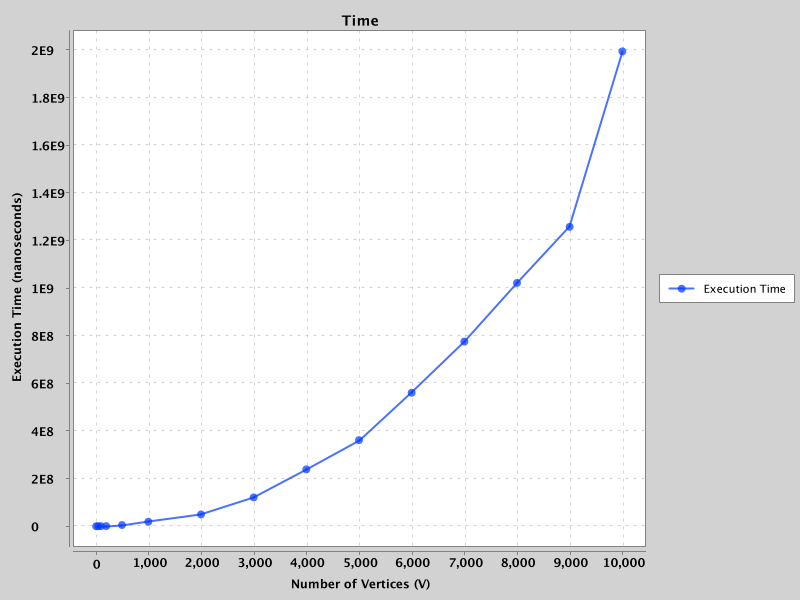
\includegraphics[width=0.6\textwidth]{Completetime.png}
        \end{center}
        Create a chart showing the running times for various values of ``$v$"
    \begin{center}
    \begin{tabular}{c|c}
    \hline
    v & times(ns)  \\
    \hline
    10 & 294583\\
    \hline
    50 & 434166\\
    \hline
    100 & 608666 \\ 
    \hline
    200 & 836625 \\ 
    \hline 
    500 & 5381125\\
    \hline
    1000 & 19269750 \\
    \hline
    2000 & 49767459 \\
    \hline
    3000 & 121378208 \\
    \hline 
    4000 & 239193292 \\
    \hline
    5000 & 361908791 \\
    \hline 
    6000 & 560953084 \\
    \hline 
    7000 & 775675041 \\
    \hline 
    8000 & 1022001459 \\
    \hline
    9000 & 1257583417 \\
    \hline
    10000 & 1994619792 \\
    \hline
    \end{tabular}
    \end{center}
    
    \item CYCLE
    The cycle graph is formed of a single cycle that contains every vertex in the graph. This is formed by iterating over every vertex and connecting it to the next one. Finally, the las vertex is connected back to the start.
    \begin{minted}
[frame=lines,framesep=2mm,baselinestretch=1.2,fontsize=\footnotesize,linenos]{java}
static class Cycle {
    static void addEdge(ArrayList<ArrayList<Integer>> am, int s, int d) {
        am.get(s).add(d);
        am.get(d).add(s);
    }
    static void allEdgeCycle(ArrayList<ArrayList<Integer>> am, int V) {
        //long startTime = System.nanoTime();
        for (int i = 0; i < V; i++) {
            if (i == V - 1) {
                addEdge(am, i, 0);   // head -- tail
            } else {
                addEdge(am, i, i + 1);
            }
        }
    }
}

    \end{minted}
    The running time: $\Theta(V)$.\\
    Use the data from $V = (100, 200, 300, ... , 100000)$
                \begin{center}
        
        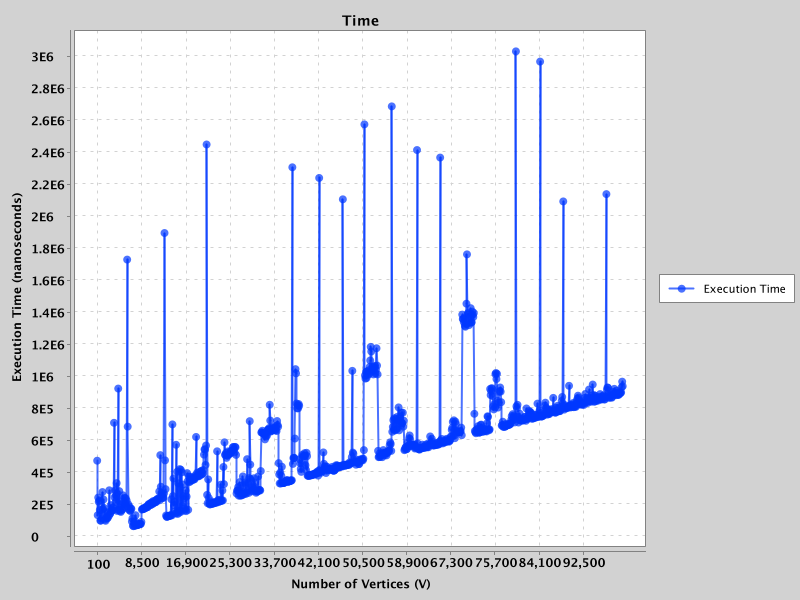
\includegraphics[width=0.6\textwidth]{cycle1.png}
        \end{center}
    Use the data from [10, 50, 100, 200, 500, 1000, 2000, 3000, 4000, 5000, 6000, 7000, 8000, 9000, 10000]
            \begin{center}
            
        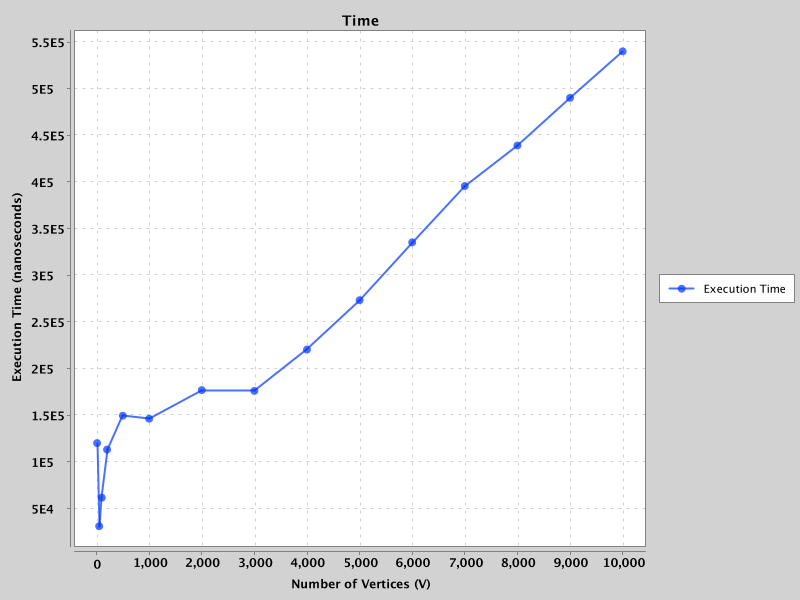
\includegraphics[width=0.6\textwidth]{cycle.png}
        \end{center}
        Create a chart showing the running times for various values of ``$v$"
    \begin{center}
    \begin{tabular}{c|c}
    \hline
    v & times(ns)  \\
    \hline 
    50 & 31083\\
    \hline
    100 & 61709\\
    \hline
    200 & 113250 \\ 
    \hline
    500 & 149541 \\ 
    \hline
    1000 & 146334\\
    \hline
    2000 & 177000 \\
    \hline
    3000 & 176125 \\
    \hline
    4000 & 220459 \\
    \hline 
    5000 & 273375 \\
    \hline
    6000 & 335333 \\
    \hline 
    7000 & 395708 \\
    \hline 
    8000 & 439167 \\
    \hline 
    9000 & 490250 \\
    \hline
    10000 & 540084 \\
    \hline
    \end{tabular}
    \end{center}
    
    \item UNIFORM
        \begin{minted}
[frame=lines,framesep=2mm,baselinestretch=1.2,fontsize=\footnotesize,linenos]{java}
    static class Uniform {

        static void addEdge(ArrayList<ArrayList<Integer>> am, int s, int d) {
            am.get(s).add(d);
            am.get(d).add(s);
        }

        // If you provide an integer parameter to "nextInt",
        // it will return an integer from a uniform distribution 
        // between 0 and one less than the parameter.
        static void uniformRandom(ArrayList<ArrayList<Integer>> am, int v, int e) {
            //Random rand = new Random();
            while (e > 0) {
                int source = (int) (Math.random() * v); // Printing the random number between [0,v-1]
                int dest = (int) (Math.random() * v);
                // edge exit?
                if (source == dest || am.get(source).contains(dest)) {
                    continue;
                } else {
                    addEdge(am, source, dest);
                    e--;
                }
            }
        }
    }
    \end{minted}
    The uniform distribution pick up the vertices looks like in the following, the x axis means the vertex total number, pick up 10000 times, and divide 10000 vertices into 12 groups:\\
    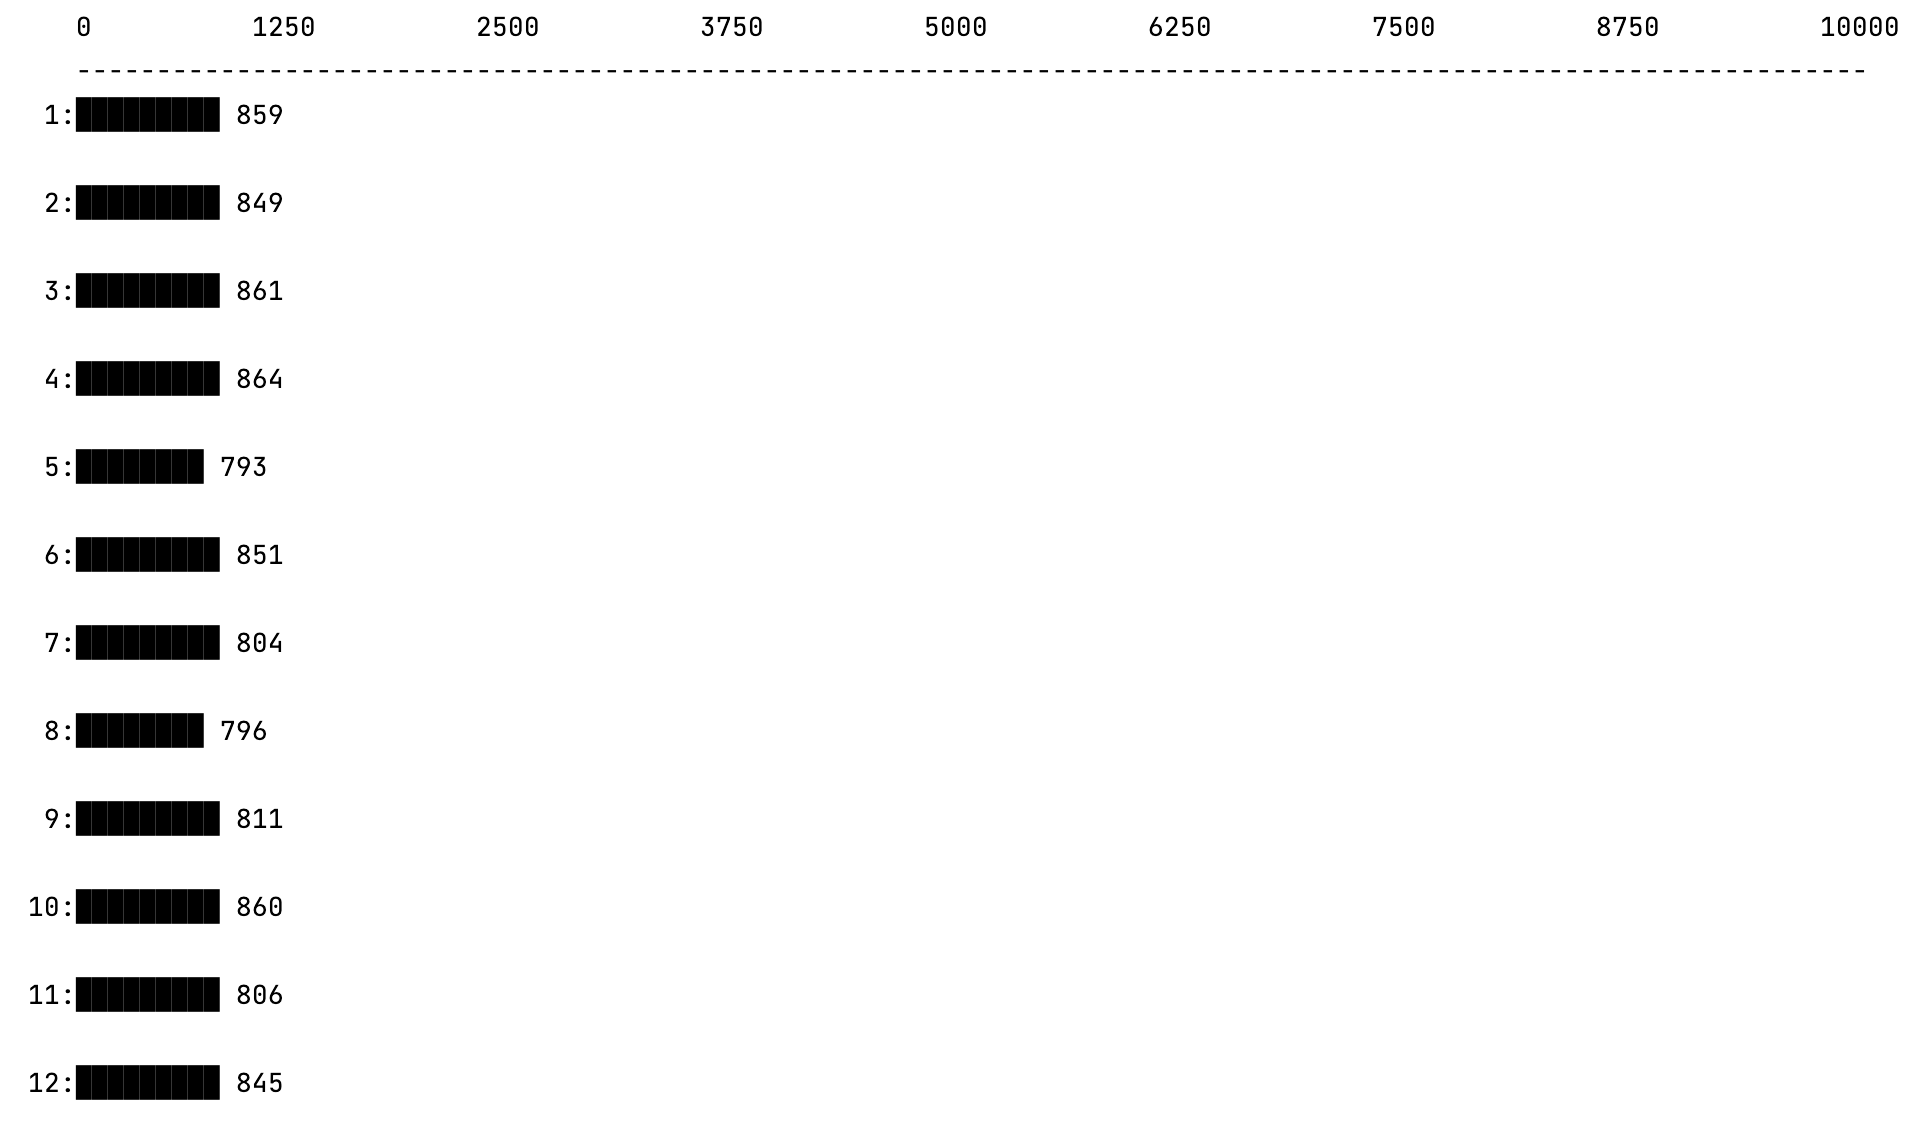
\includegraphics[width=0.9\textwidth]{uniform.png}

    The running time : $\Theta(V \times E)$\\
    Use the data from $V = (100, 200, 300, ... , 100000)$, and different edges as test to run:\\
    $E = \frac{V}{8}$: 
                    \begin{center}
        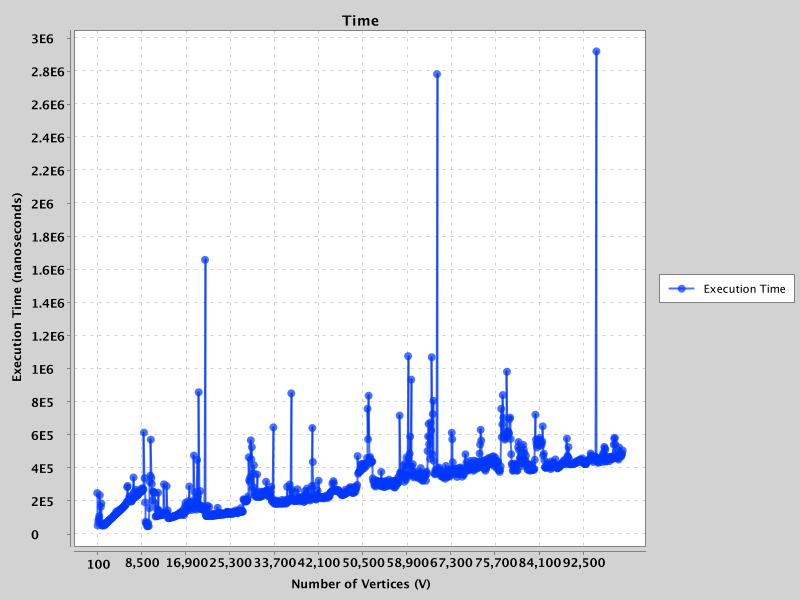
\includegraphics[width=0.6\textwidth]{un18.png}
        \end{center}
    $E = \frac{V}{4}$: 
                    \begin{center}
        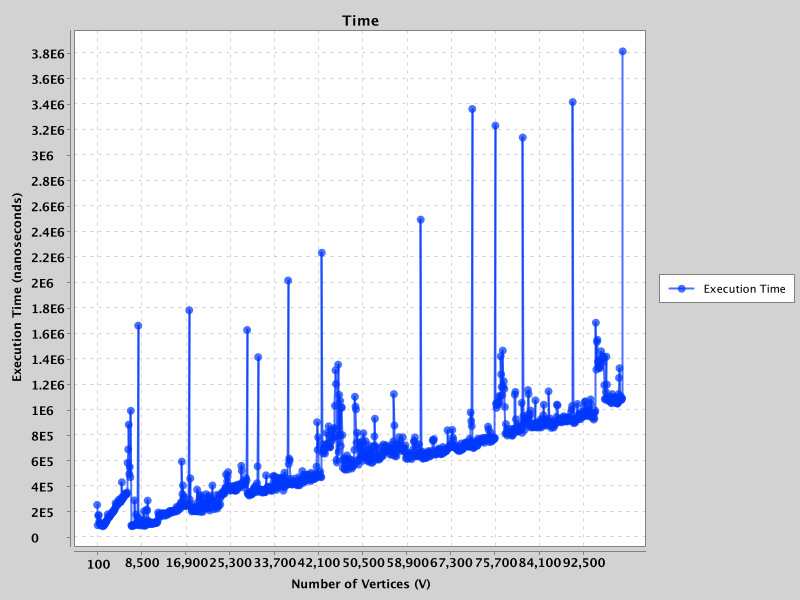
\includegraphics[width=0.6\textwidth]{un14.png}
        \end{center}
    $E = \frac{V}{2}$
                \begin{center}
        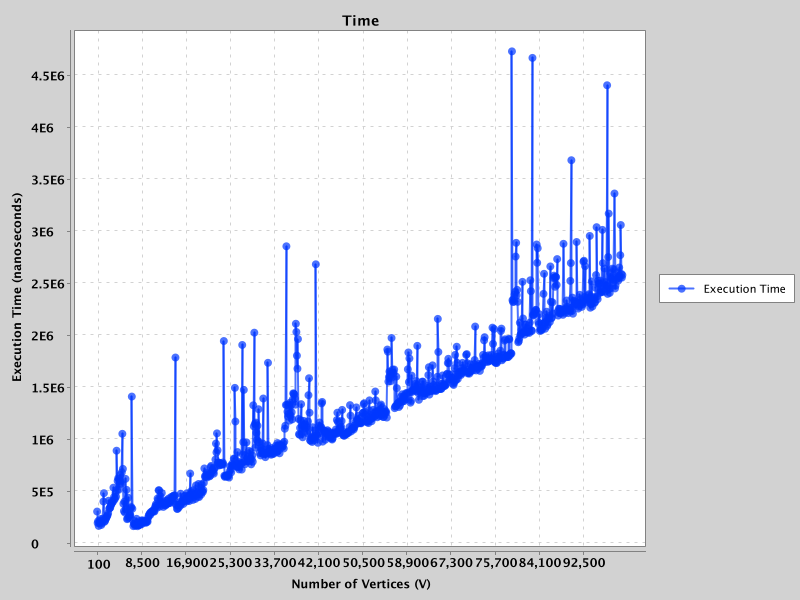
\includegraphics[width=0.6\textwidth]{uniformtime.png}
        \end{center}
    $E = V$: 
        \begin{center}
        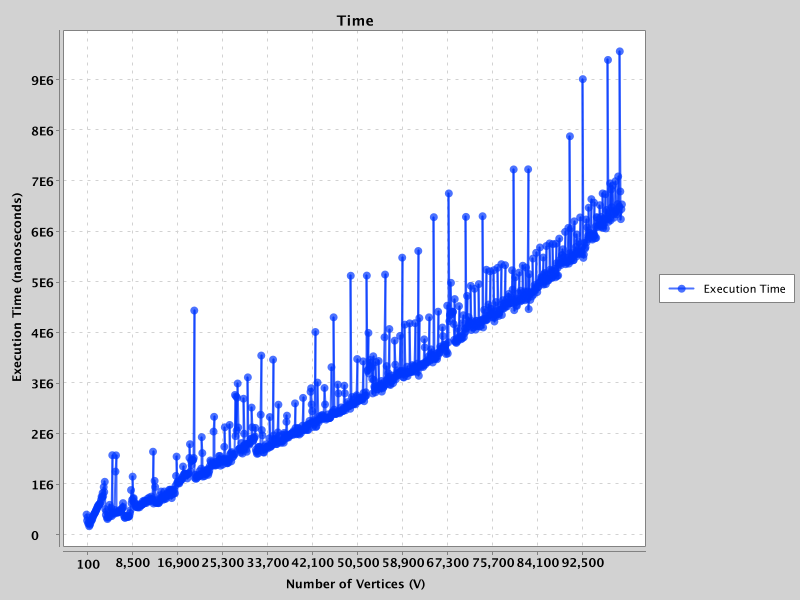
\includegraphics[width=0.6\textwidth]{univ.png}
        \end{center}
    $E = 2V$: 
        \begin{center}
        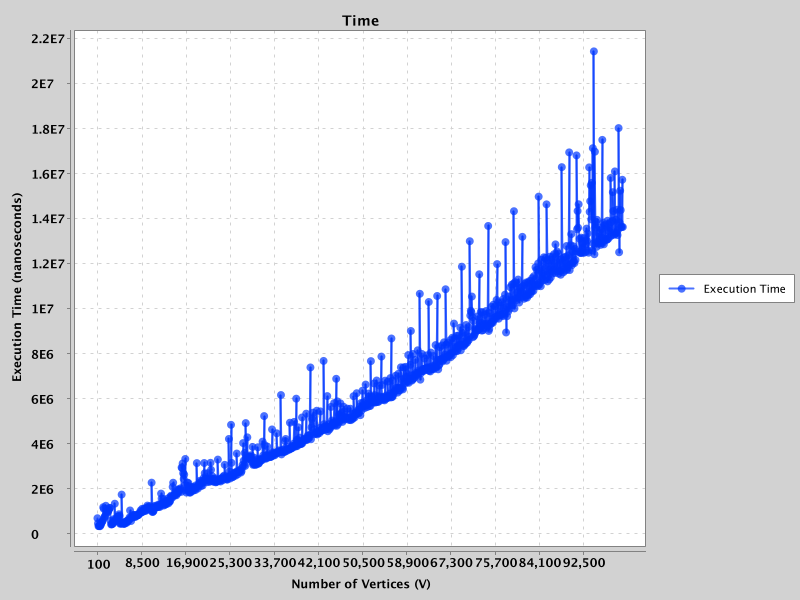
\includegraphics[width=0.6\textwidth]{uni2v.png}
        \end{center}
        $E = 4V$: 
        \begin{center}
        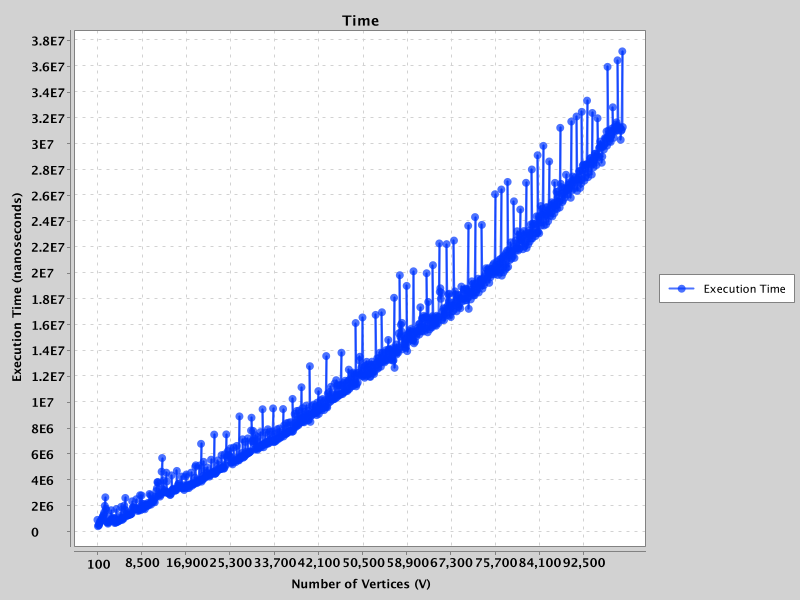
\includegraphics[width=0.6\textwidth]{uni4v.png}
        \end{center}
    $E = 8V$ 
                    \begin{center}
        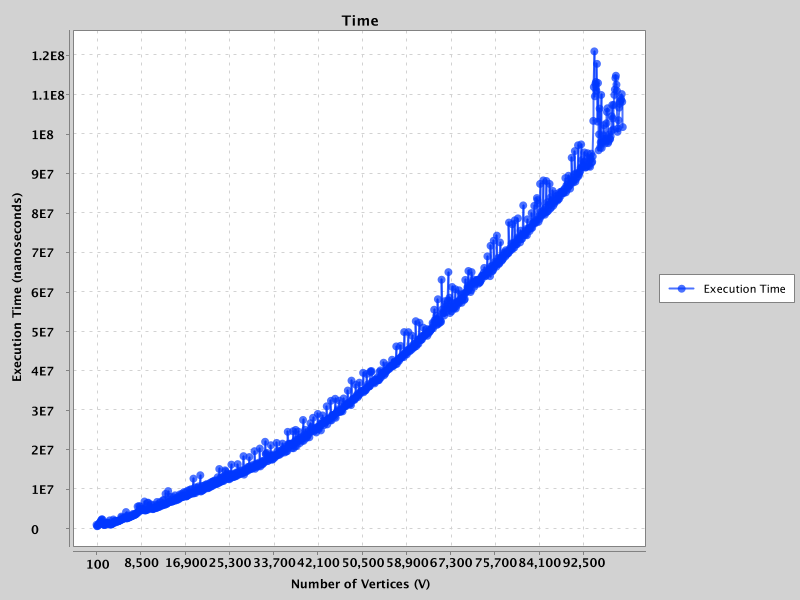
\includegraphics[width=0.6\textwidth]{uniform8V.png}
        \end{center}
    
    \item SKEWED
            \begin{minted}
[frame=lines,framesep=2mm,baselinestretch=1.2,fontsize=\footnotesize,linenos]{java}
    static class Skewed {
        static void addEdge(ArrayList<ArrayList<Integer>> am, int s, int d) {
            am.get(s).add(d);
            am.get(d).add(s);
        }

        static void skewedRandom(ArrayList<ArrayList<Integer>> am, int v, int e) {
            int source = -1;
            int dest = -1;
            int a = 0;
            int b = v;
            int c = 0;
            double F = (c - a) / (b - a);
            while (e > 0) {
                double rand = Math.random();
                if (rand < F) {
                    source = (int) (a + Math.sqrt(rand * (b - a) * (c - a)));
                } else {
                    source = (int) (b - Math.sqrt((1 - rand) * (b - a) * (b - c)));
                }

                double rand2 = Math.random();
                if (rand2 < F) {
                    dest = (int) (a + Math.sqrt(rand2 * (b - a) * (c - a)));
                } else {
                    dest = (int) (b - Math.sqrt((1 - rand2) * (b - a) * (b - c)));
                }

                if (source == dest || am.get(source).contains(dest)) {
                    continue;
                } else {
                    addEdge(am, source, dest);
                    e--;
                }
            }

        }
    }
    \end{minted}
        The skewed distribution pick up the vertices looks like in the following, the x axis means the vertex total number, pick up 10000 times, and divide 10000 vertices into 12 groups:\\
        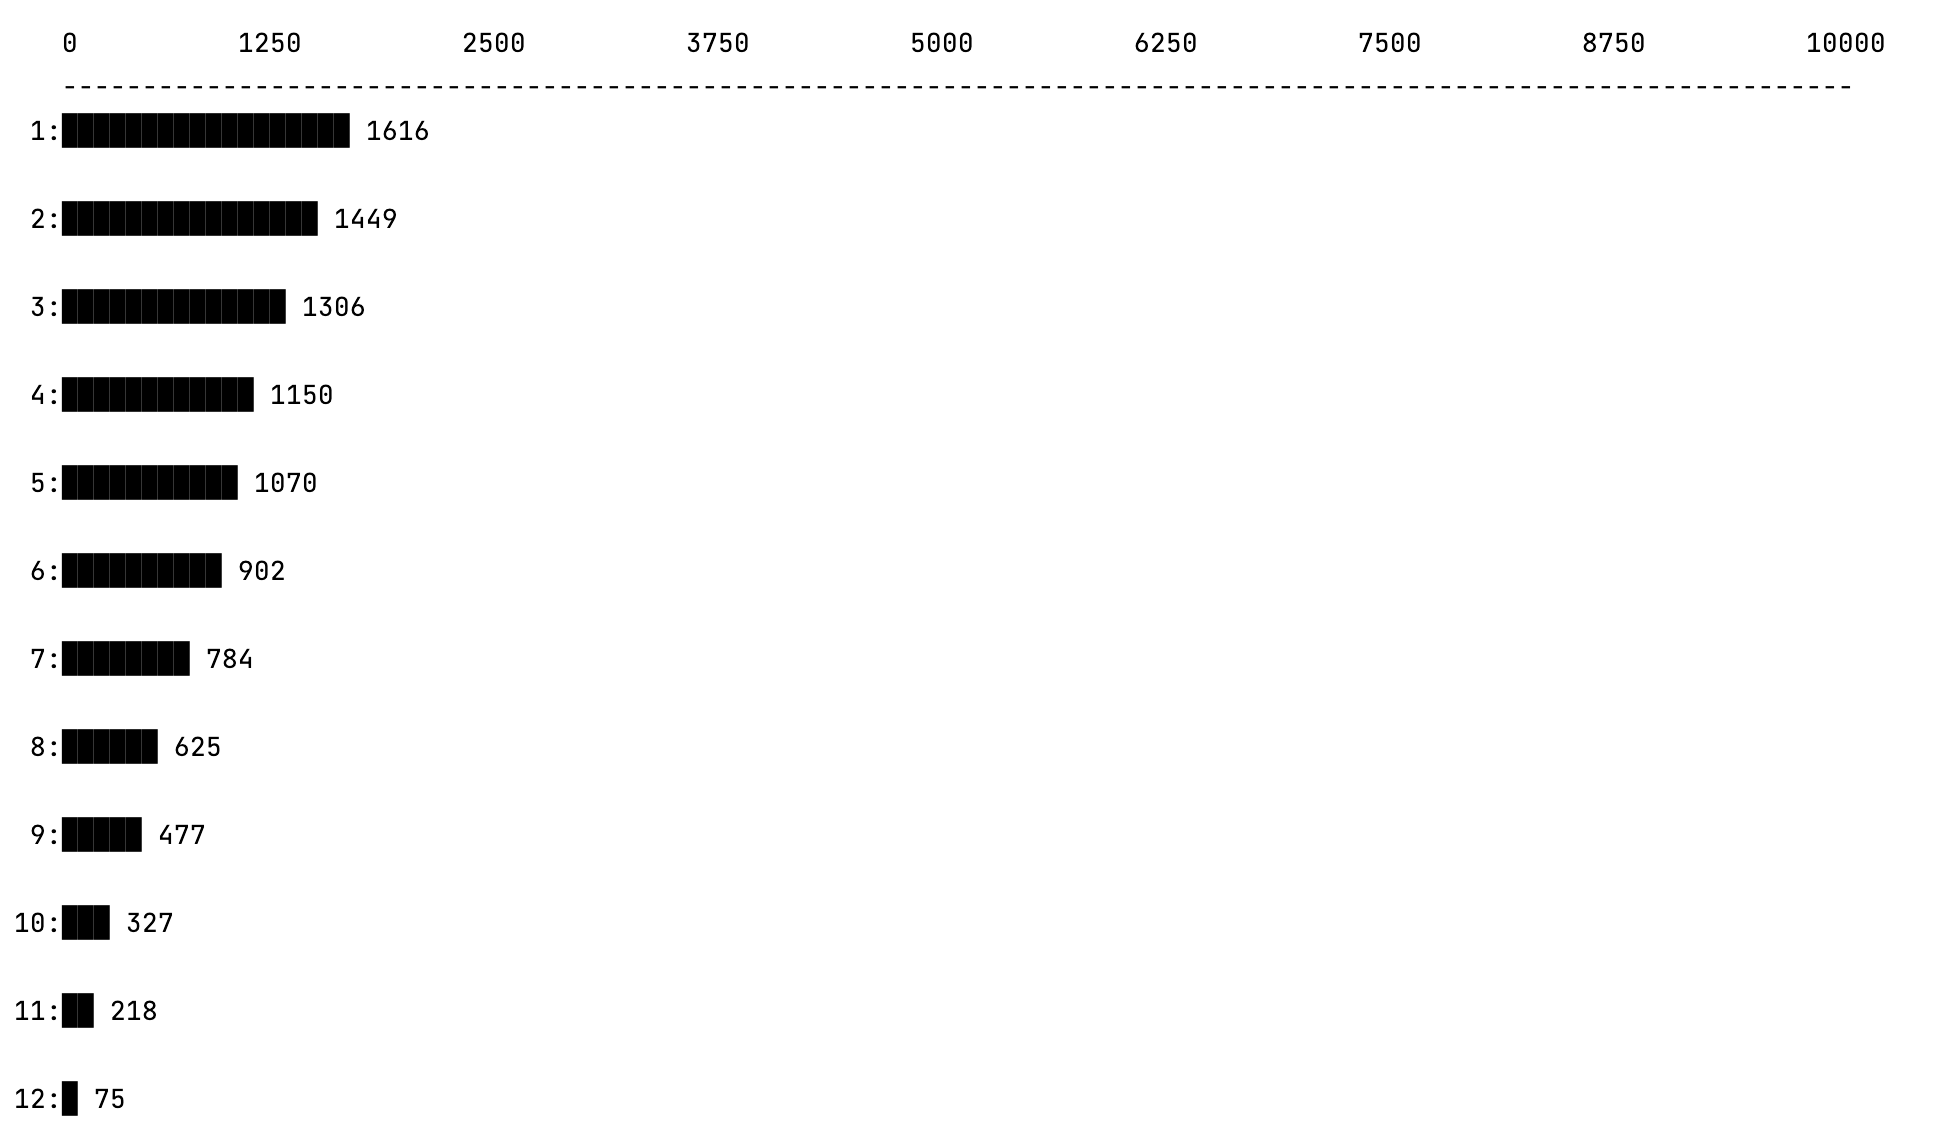
\includegraphics[width=0.9\textwidth]{skewed.png}
        
    The running time : $\Theta(V \times E)$\\
    Use the data from $V = (100, 200, 300, ... , 100000)$, and different edges as test to run:\\
    $E = \frac{V}{8}$: 
                    \begin{center}
        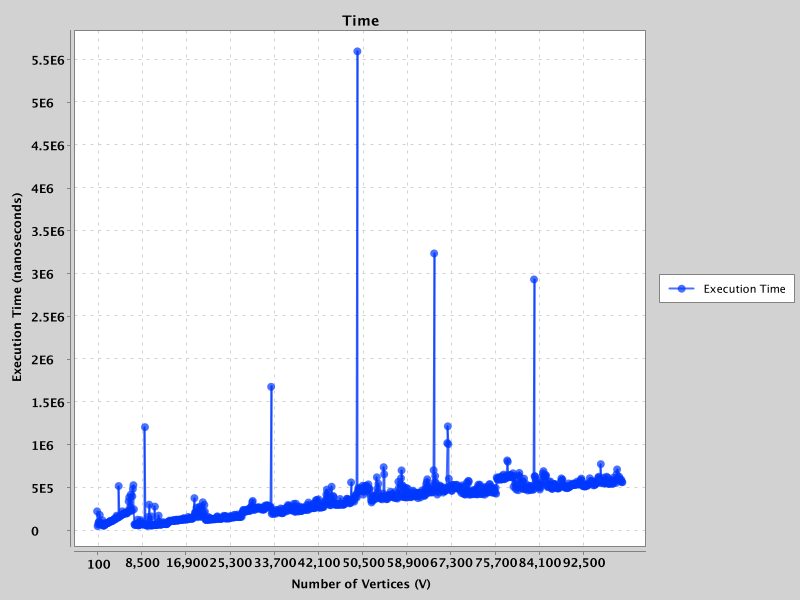
\includegraphics[width=0.6\textwidth]{s1.png}
        \end{center}
    $E = \frac{V}{4}$: 
                    \begin{center}
        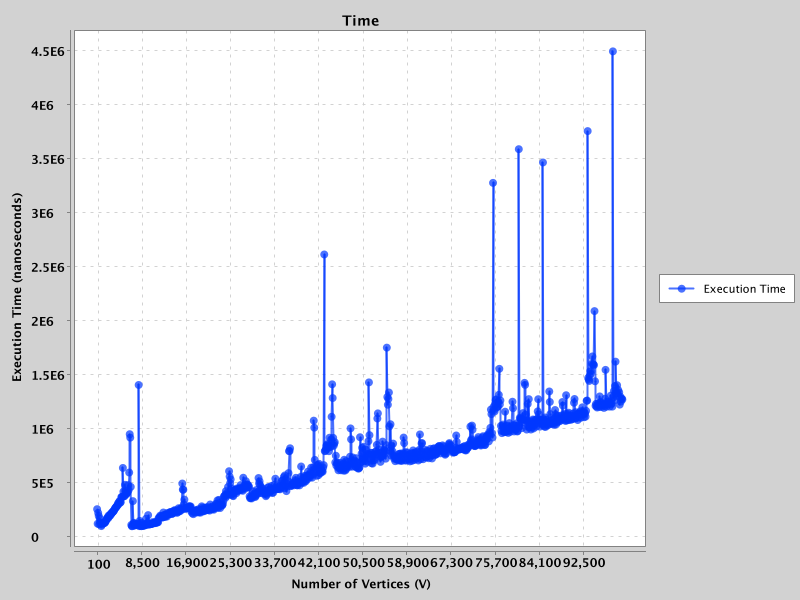
\includegraphics[width=0.6\textwidth]{s2.png}
        \end{center}
    $E = \frac{V}{2}$
                \begin{center}
        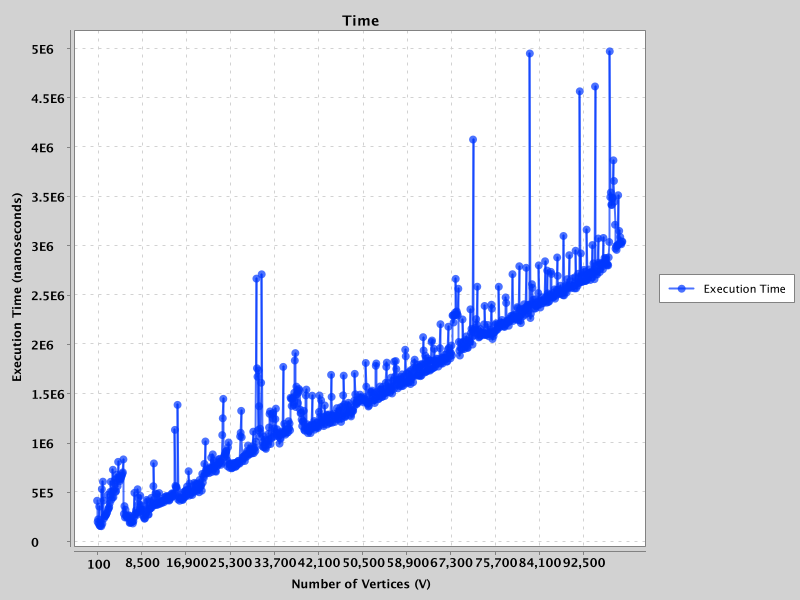
\includegraphics[width=0.6\textwidth]{s3.png}
        \end{center}
    $E = V$: 
        \begin{center}
        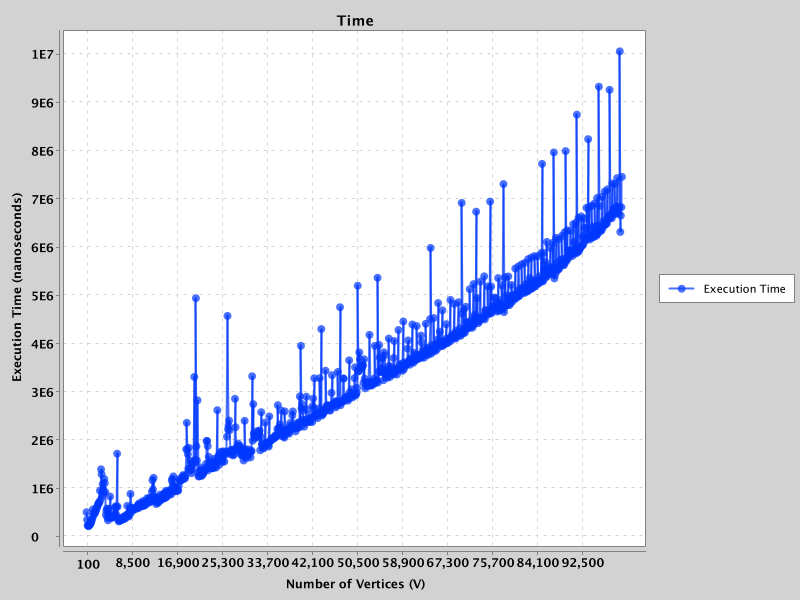
\includegraphics[width=0.6\textwidth]{s4.png}
        \end{center}
    $E = 2V$: 
        \begin{center}
        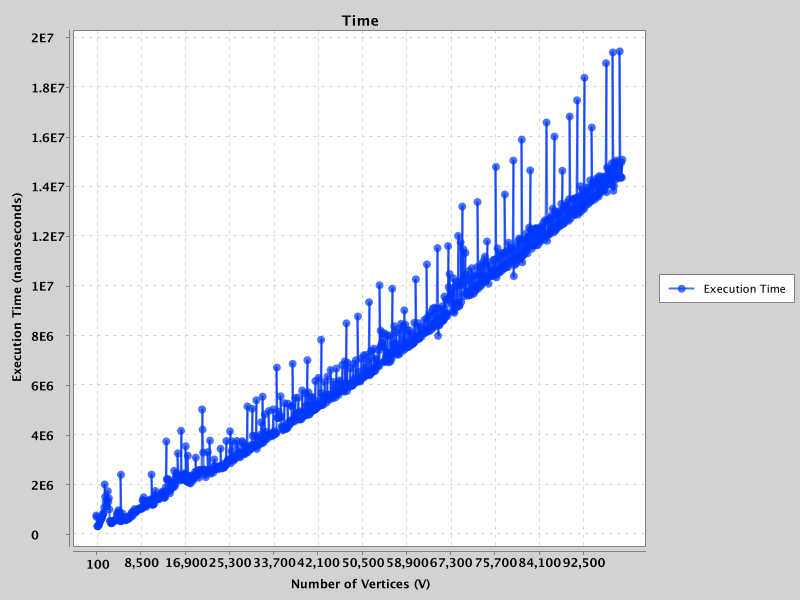
\includegraphics[width=0.6\textwidth]{s5.png}
        \end{center}
        $E = 4V$: 
        \begin{center}
        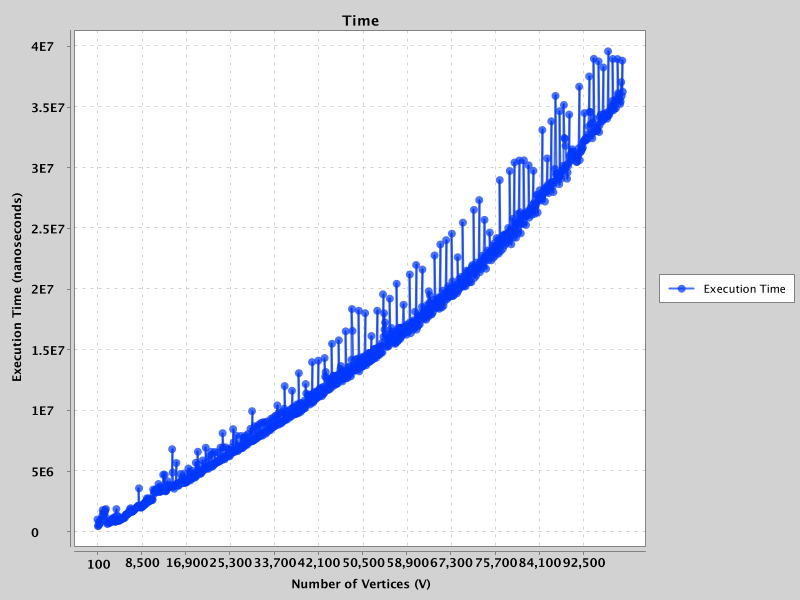
\includegraphics[width=0.6\textwidth]{s6.png}
        \end{center}
    $E = 8V$ 
                    \begin{center}
        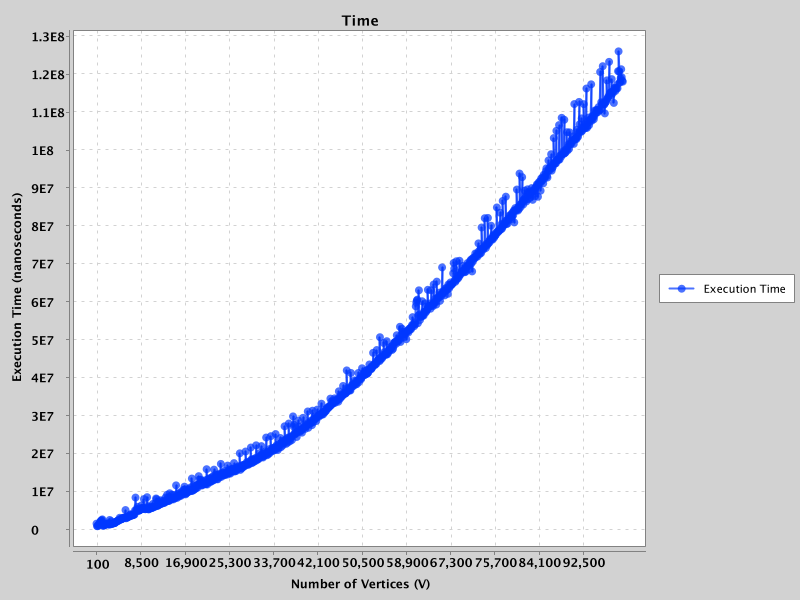
\includegraphics[width=0.6\textwidth]{s7.png}
        \end{center}
    
    \item GAUSS
                \begin{minted}
[frame=lines,framesep=2mm,baselinestretch=1.2,fontsize=\footnotesize,linenos]{java}
    static class Gauss {

        static void addEdge(ArrayList<ArrayList<Integer>> am, int s, int d) {
            am.get(s).add(d);
            am.get(d).add(s);
        }

        static void gaussRandom(ArrayList<ArrayList<Integer>> am, int v, int e) {
            Random rand = new Random();
            while (e > 0) {

                int source = (int) (v / 10 * rand.nextGaussian() + v / 2);
                int dest = (int) (v / 10 * rand.nextGaussian() + v / 2);

                if (source == dest || am.get(source).contains(dest)) {
                    continue;
                } else {
                    addEdge(am, source, dest);
                    e--;
                }
            }
        }
    \end{minted}
    The guass distribution pick up the vertices looks like in the following, the x axis means the vertex total number, pick up 10000 times, and divide 10000 vertices into 12 groups:\\
        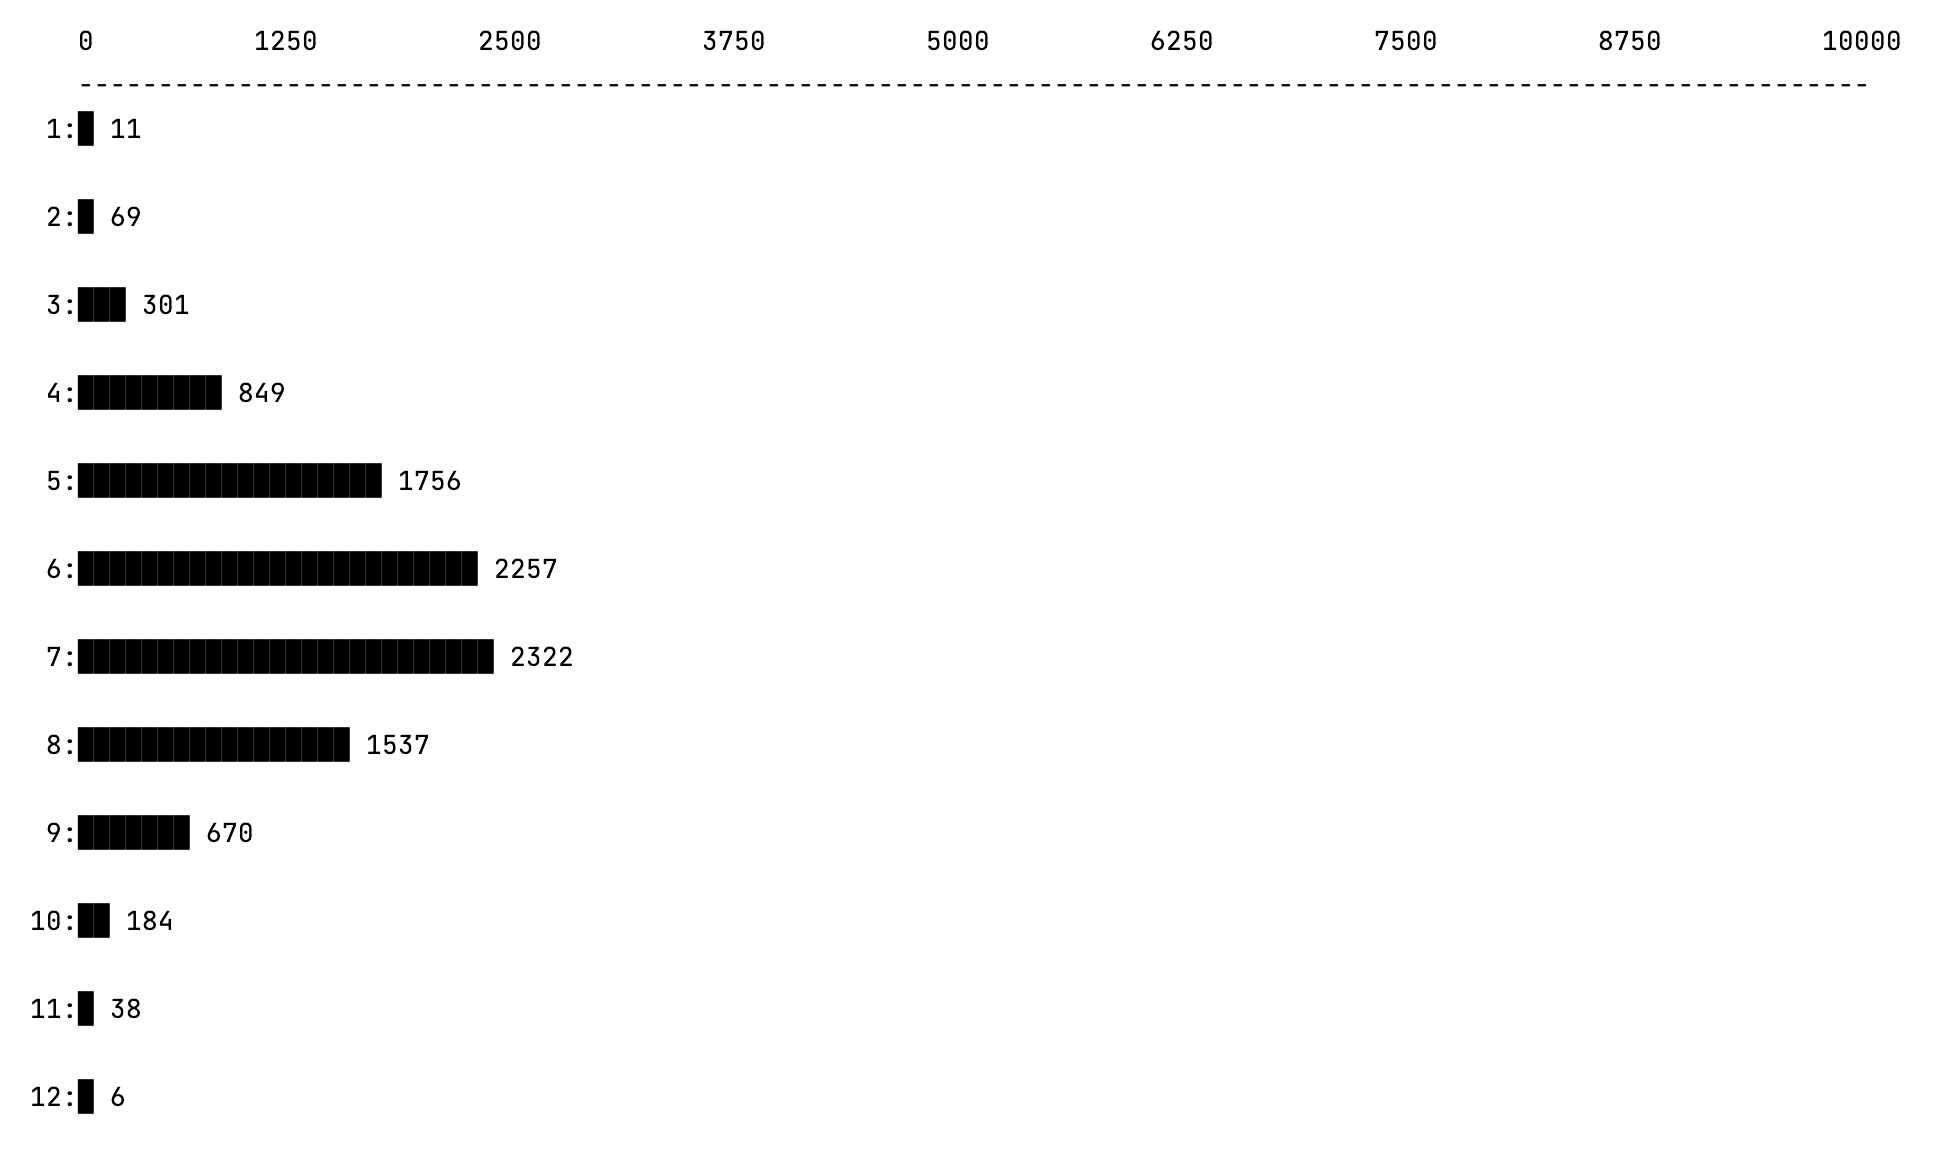
\includegraphics[width=0.9\textwidth]{gauss.png}
        
    The running time : $\Theta(V \times E)$\\
    Use the data from $V = (100, 200, 300, ... , 100000)$, and different edges as test to run:\\
    $E = \frac{V}{8}$: 
                    \begin{center}
        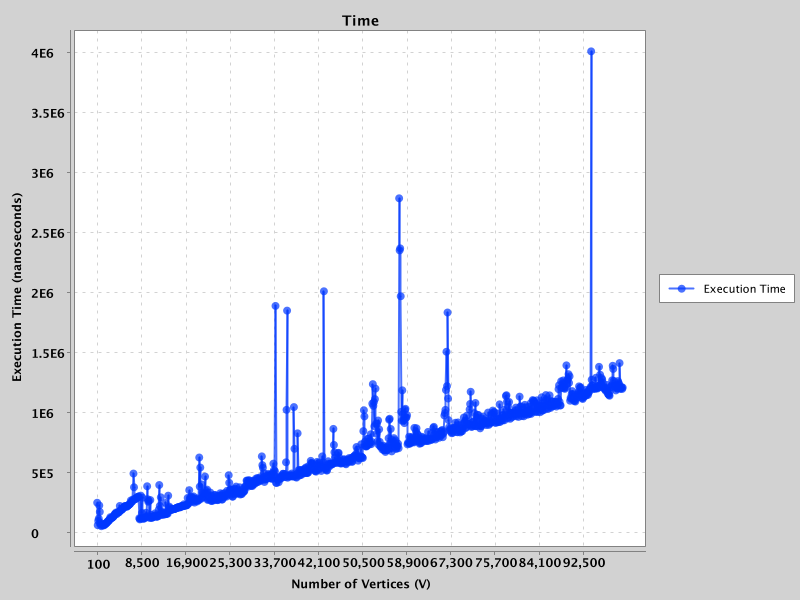
\includegraphics[width=0.6\textwidth]{g1.png}
        \end{center}
    $E = \frac{V}{4}$: 
                    \begin{center}
        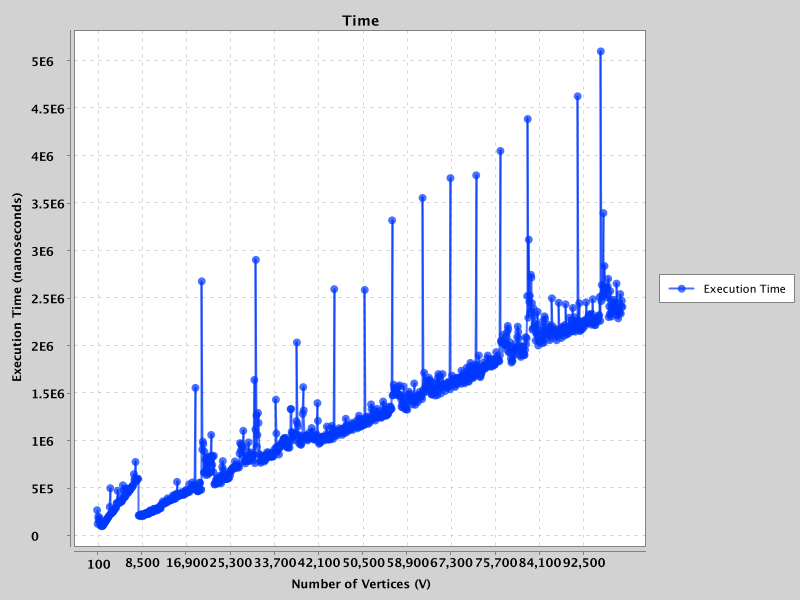
\includegraphics[width=0.6\textwidth]{g2.png}
        \end{center}
    $E = \frac{V}{2}$
                \begin{center}
        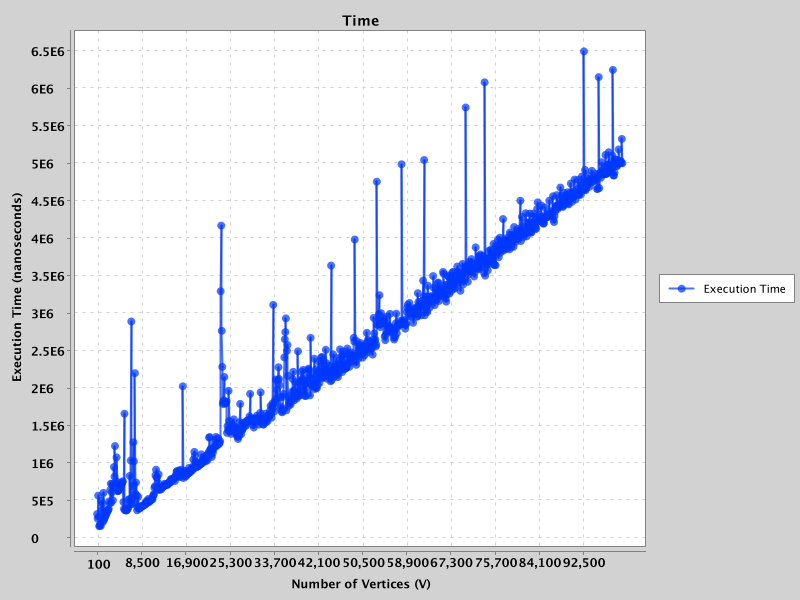
\includegraphics[width=0.6\textwidth]{g3.png}
        \end{center}
    $E = V$: 
        \begin{center}
        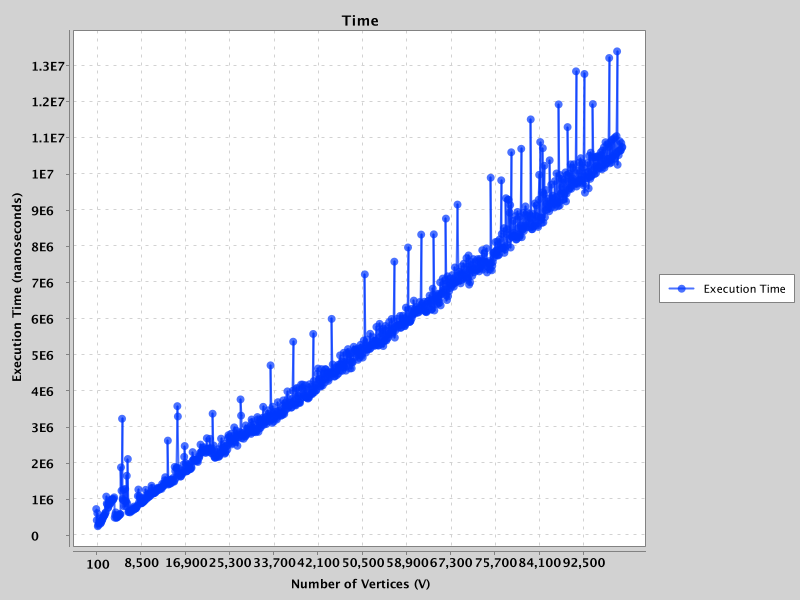
\includegraphics[width=0.6\textwidth]{g4.png}
        \end{center}
    $E = 2V$: 
        \begin{center}
        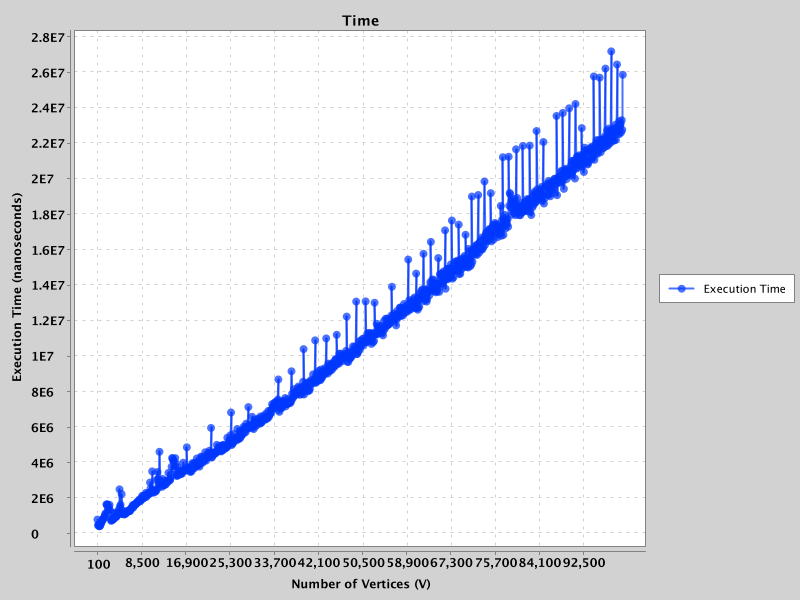
\includegraphics[width=0.6\textwidth]{g5.png}
        \end{center}
        $E = 4V$: 
        \begin{center}
        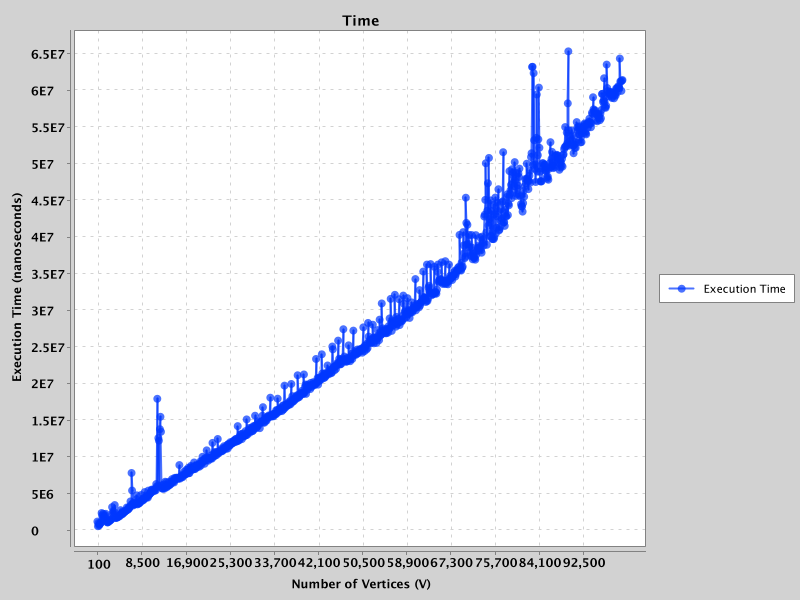
\includegraphics[width=0.6\textwidth]{g6.png}
        \end{center}
    $E = 8V$ 
                    \begin{center}
        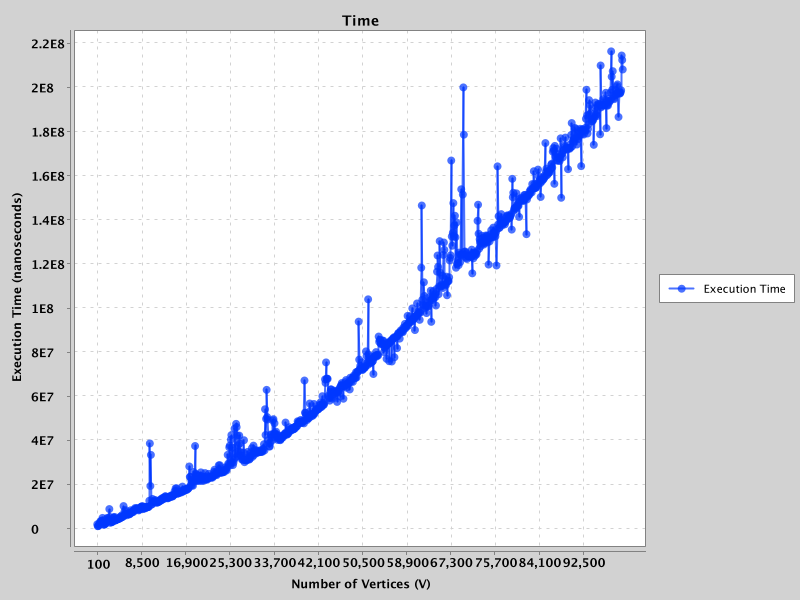
\includegraphics[width=0.6\textwidth]{g7.png}
        \end{center}
\end{enumerate}
\subsubsection{Histograms showing how many conflicts each vertex has for each method}
To create histograms showing the number of conflicts (degree) each vertex has for each method, I use the XChart library to create the histograms. I use $v = 100, E = 200$ as example, the result in the following:
    \begin{center}

        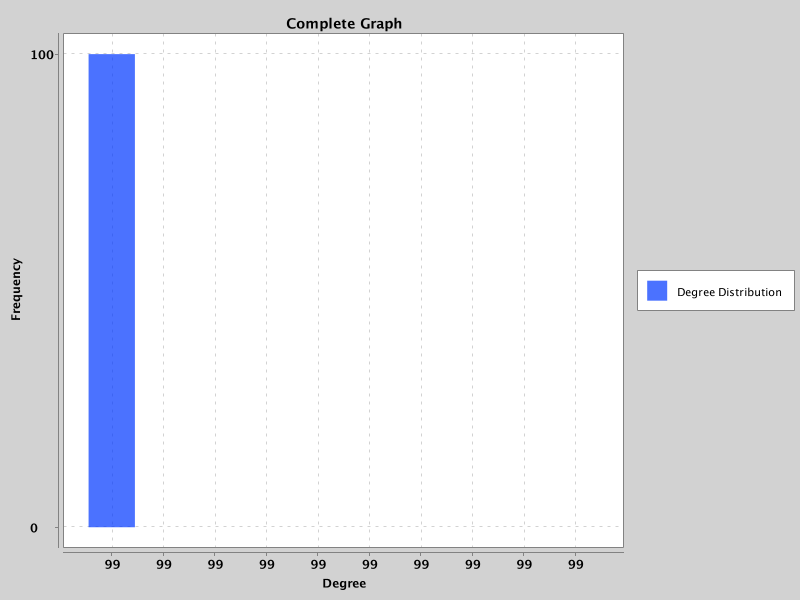
\includegraphics[width=0.6\textwidth]{c2.png}
        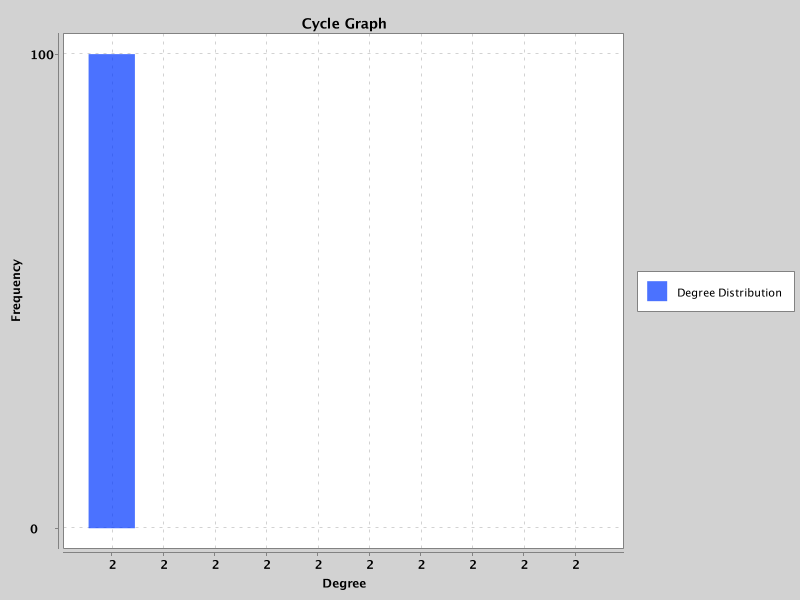
\includegraphics[width=0.6\textwidth]{c1.png}
        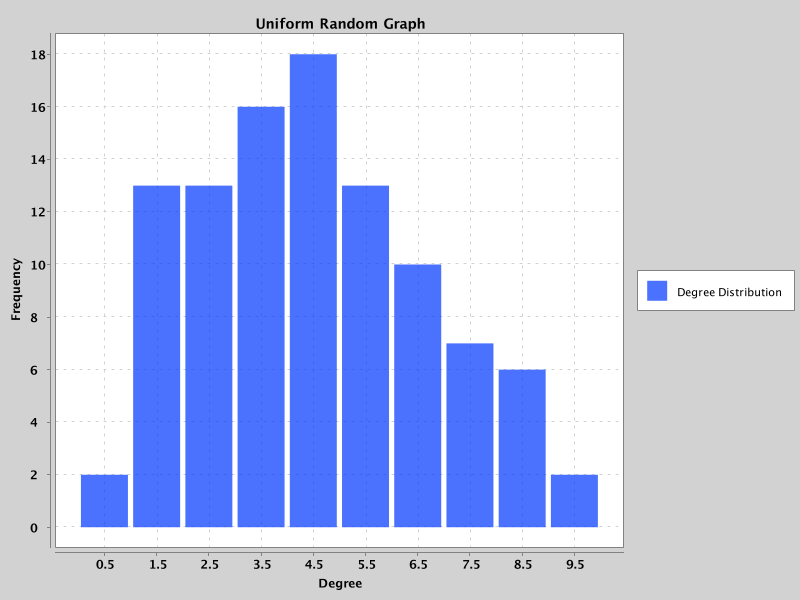
\includegraphics[width=0.6\textwidth]{c3.png}
        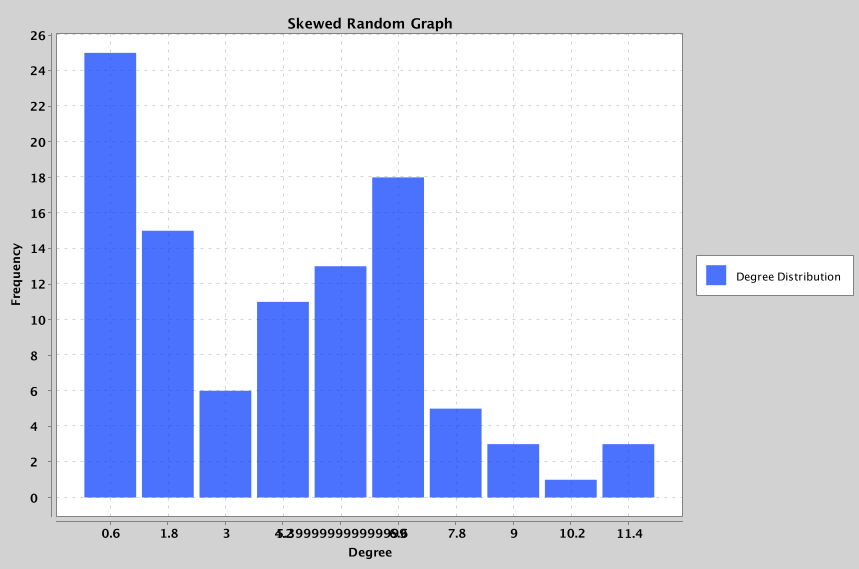
\includegraphics[width=0.6\textwidth]{c4.png}
        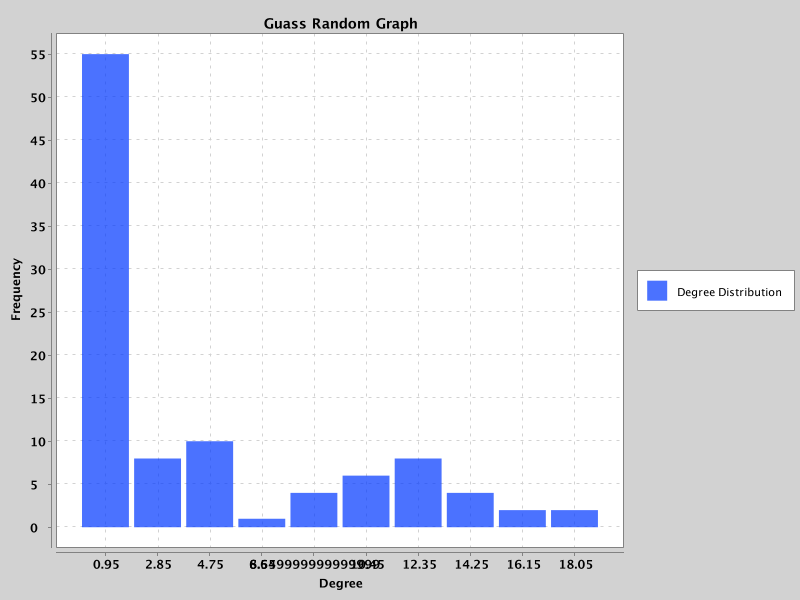
\includegraphics[width=0.6\textwidth]{c5.png}
    \end{center}

\section{Part Two}
\subsection{Vertex Ordering}
In these part, I use three graph as example: \\
Example 1: \\
    \begin{center}
        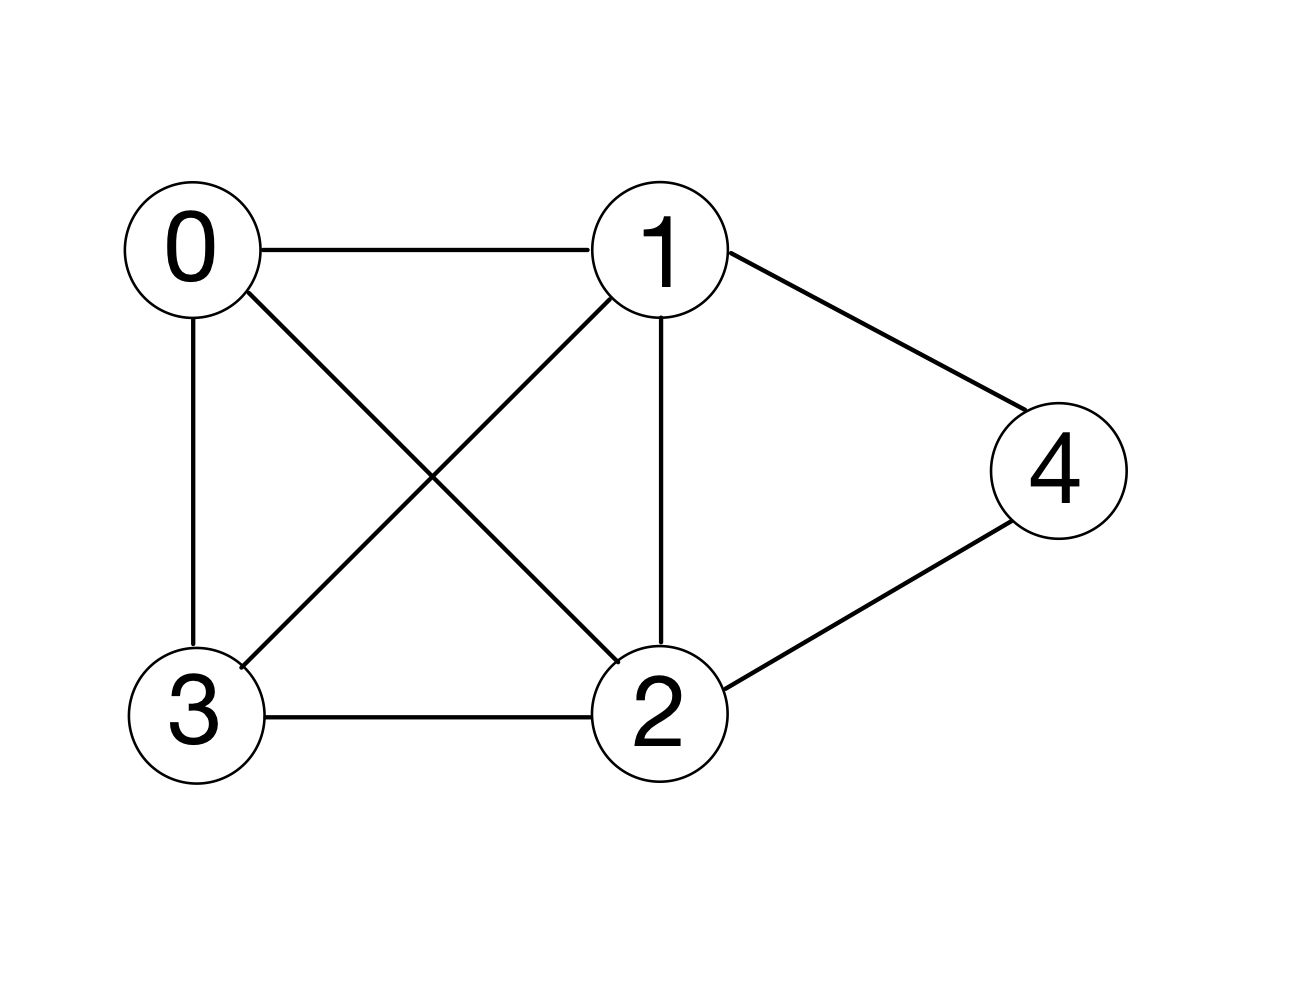
\includegraphics[width=0.3\textwidth]{p33.jpeg}
    \end{center}
Example 2: \\
    \begin{center}
        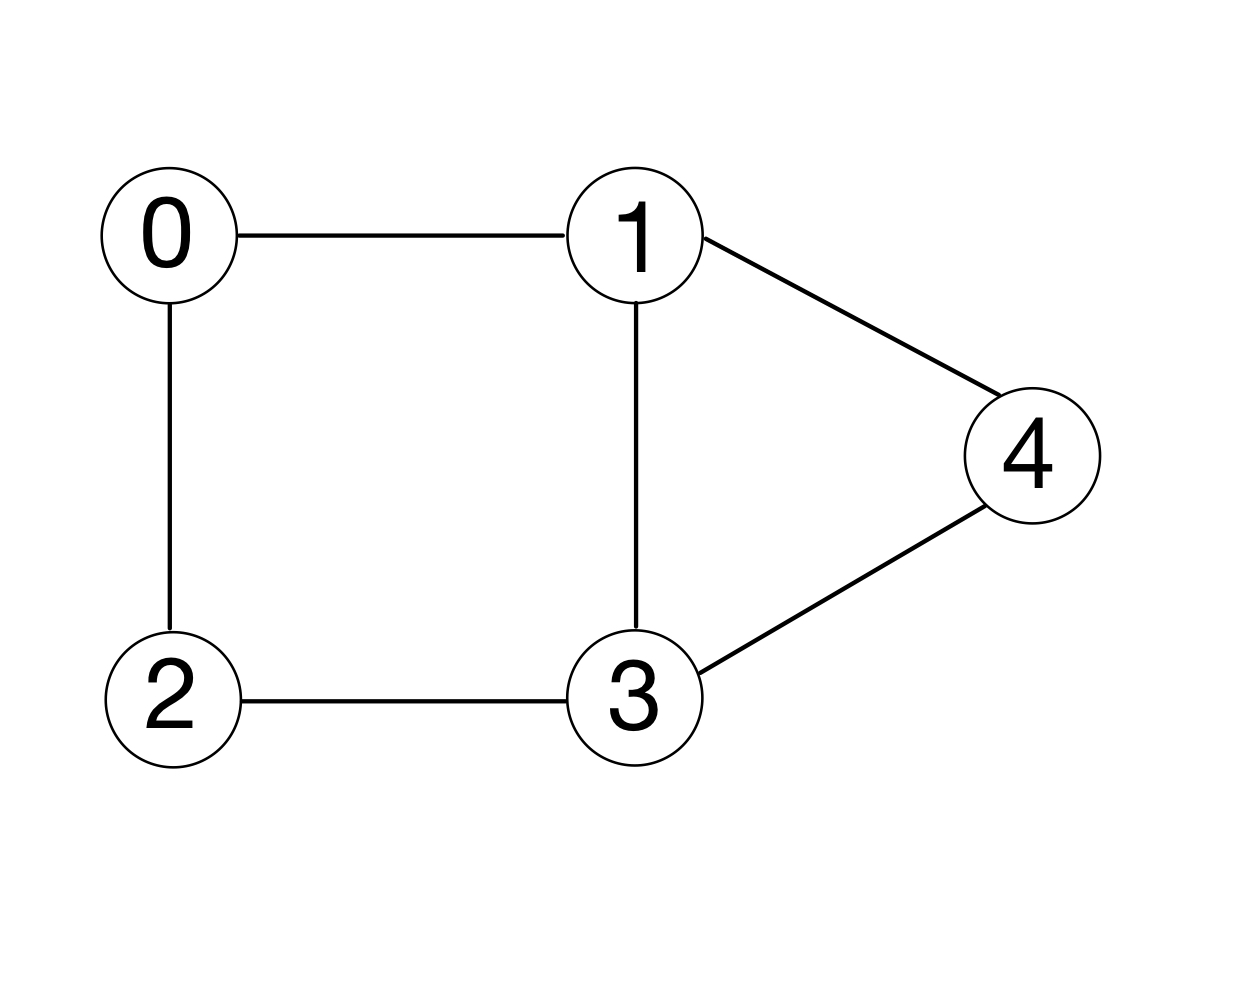
\includegraphics[width=0.3\textwidth]{p44.jpeg}
    \end{center}
Example 3: \\    
    \begin{center}
        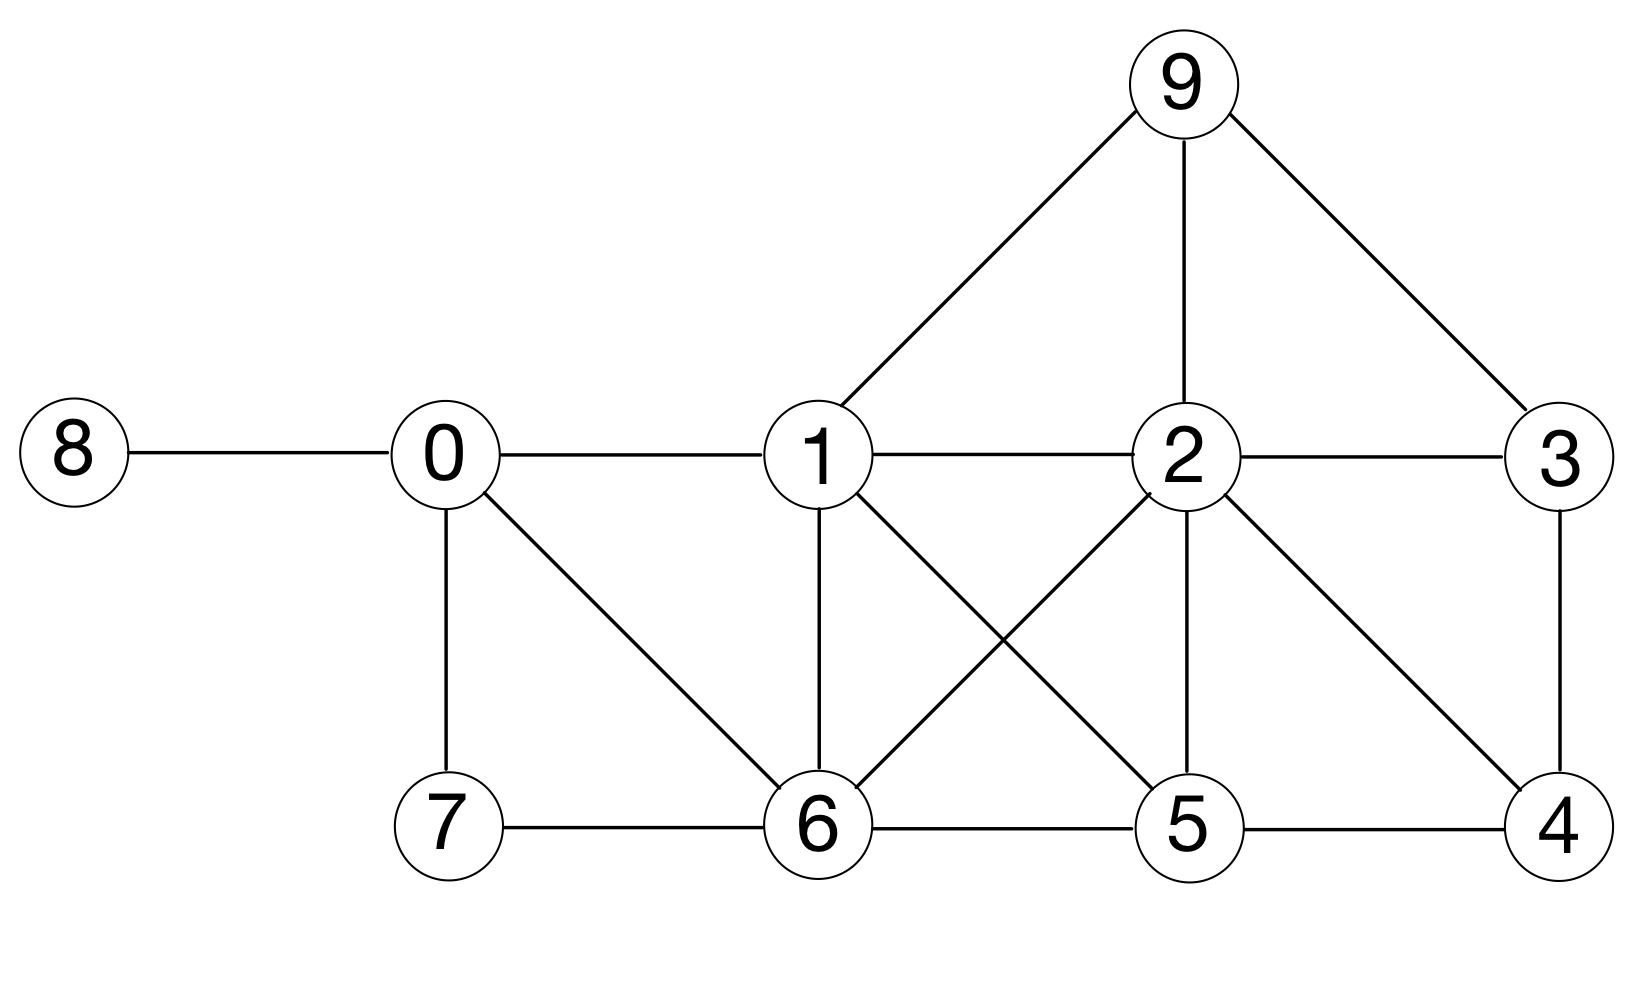
\includegraphics[width=0.5\textwidth]{p55.jpeg}
    \end{center}  
\begin{enumerate}

\item Smallest Last Vertex (SLV) Ordering: This algorithm aims to order the vertices in a way that the vertex with the smallest degree comes last. The process is repeated for the remaining vertices until all vertices are ordered. SLV ordering is mainly used for graph coloring and reducing the fill-in of sparse matrices.
    \begin{minted}
[frame=lines,framesep=2mm,baselinestretch=1.2,fontsize=\footnotesize,linenos]{java}
    // Method 1: Smallest Last Vertex (SLV) Ordering:
    public static int terminalclique;
    public static int maxdegree;
    public static void removeVertex(int vertex, ArrayList<ArrayList<Integer>> am) {
        for (int i = 0; i < am.size(); i++) {
            am.get(i).remove((Integer) vertex);
        }
        am.set(vertex, new ArrayList<>());
    }

    public static int findSmallestDegreeVertex(ArrayList<ArrayList<Integer>> am) {
        int minDegree = Integer.MAX_VALUE;
        int minDegreeVertex = -1;

        for (int i = 0; i < am.size(); i++) {
            int degree = am.get(i).size();

            System.out.println("The degree of Vertex " + i + ": " + degree);
            if (degree < minDegree && degree > 0) {
                minDegree = degree;
                minDegreeVertex = i;

            }
        }

        return minDegreeVertex;
    }

    public static ArrayList<ArrayList<Integer>> copy(ArrayList<ArrayList<Integer>> am){
        ArrayList<ArrayList<Integer>> am2 = new ArrayList<ArrayList<Integer>>();
        for (int i = 0; i < am.size(); i++){
            am2.add(am.get(i));
        }

        return am2;
    }

    public static ArrayList<Integer> smallestLastVertexOrdering(ArrayList<ArrayList<Integer>> originalam) {
        ArrayList<ArrayList<Integer>> am = copy(originalam);
        ArrayList<Integer> slvOrder = new ArrayList<>();
        int res = -1;
        maxdegree = -1;
        terminalclique = -1;

        while (slvOrder.size() < am.size()) {
            printAdjacencyList(am);
            int minDegreeVertex = findSmallestDegreeVertex(am);

            if (minDegreeVertex == -1) {
                slvOrder.add(0, res);
                break;
            }

            System.out.println("The min degree Vertex is (will be deleted): " + minDegreeVertex);
            System.out.println();

            if (am.get(minDegreeVertex).size() > maxdegree){
                maxdegree = am.get(minDegreeVertex).size();
            }

            if (terminalclique < am.get(minDegreeVertex).size() &&
                    ((am.size()-slvOrder.size()-1) == am.get(minDegreeVertex).size())){
                terminalclique = am.get(minDegreeVertex).size();
            }


            slvOrder.add(0, minDegreeVertex);
            System.out.println(slvOrder);
            if (am.get(minDegreeVertex).size() == 1){
                res = am.get(minDegreeVertex).get(0);
            }
            removeVertex(minDegreeVertex,am);

        }
        System.out.println("The order to delete (from right to left): " + slvOrder);
        return slvOrder;
    }

    \end{minted}
    The running time: $\Theta(v)$


\textbf{          Example 1:}
    \begin{center}
  
        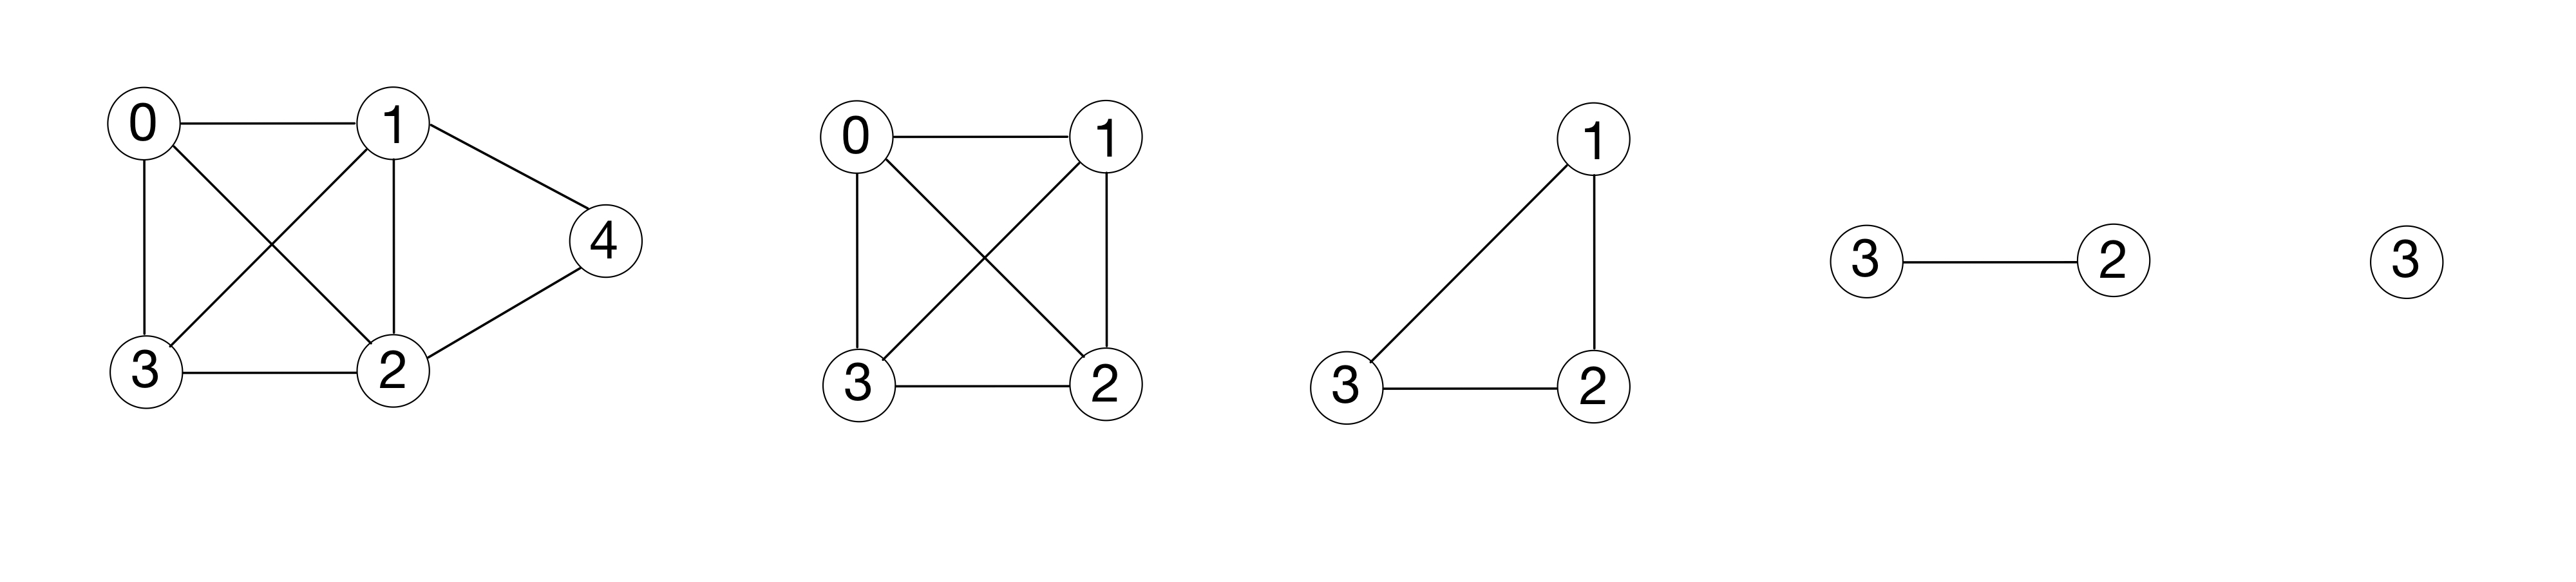
\includegraphics[width=0.9\textwidth]{ex1.jpeg}
        \begin{tabular}{|c|c|c|c|c|c|}
        \hline
            Degrees & 0&1& 2& 3&  2\\
            \hline
            Vertex & 3& 2&1& 0&   4\\ 
            \hline
        \end{tabular}
        \end{center}
\textbf{Example 2:}
\begin{center}

        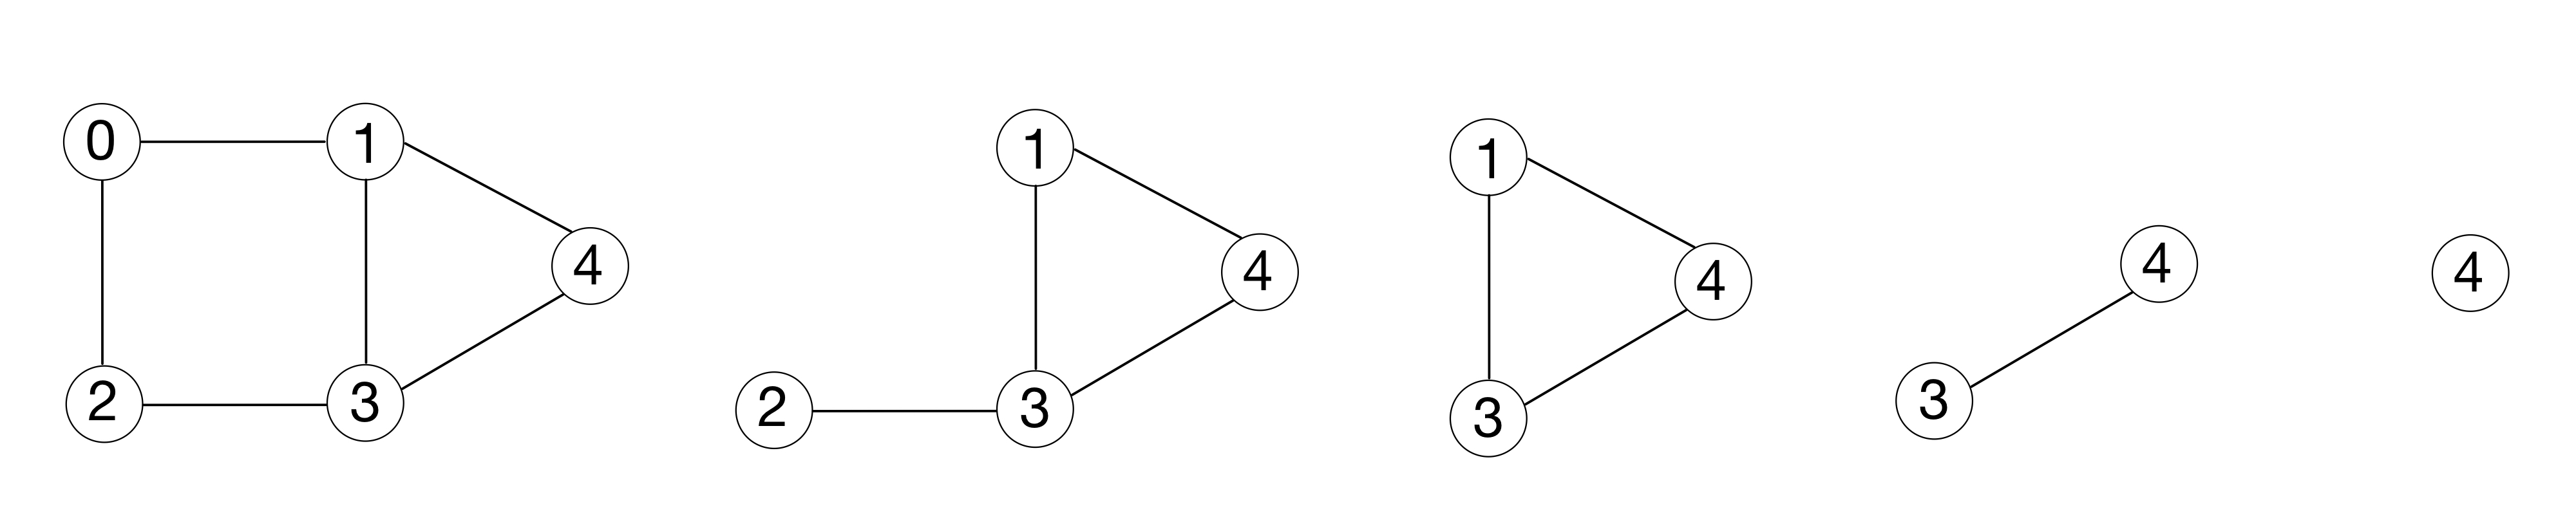
\includegraphics[width=0.9\textwidth]{Ex2.jpeg}
                \begin{tabular}{|c|c|c|c|c|c|}
        \hline
            Degrees & 0&1& 2& 1&  2\\
            \hline
            Vertex & 4& 3& 1& 2&   0\\ 
            \hline
        \end{tabular}
        \\
   \end{center}     
     \textbf{   Example 3:}
     \begin{center}
    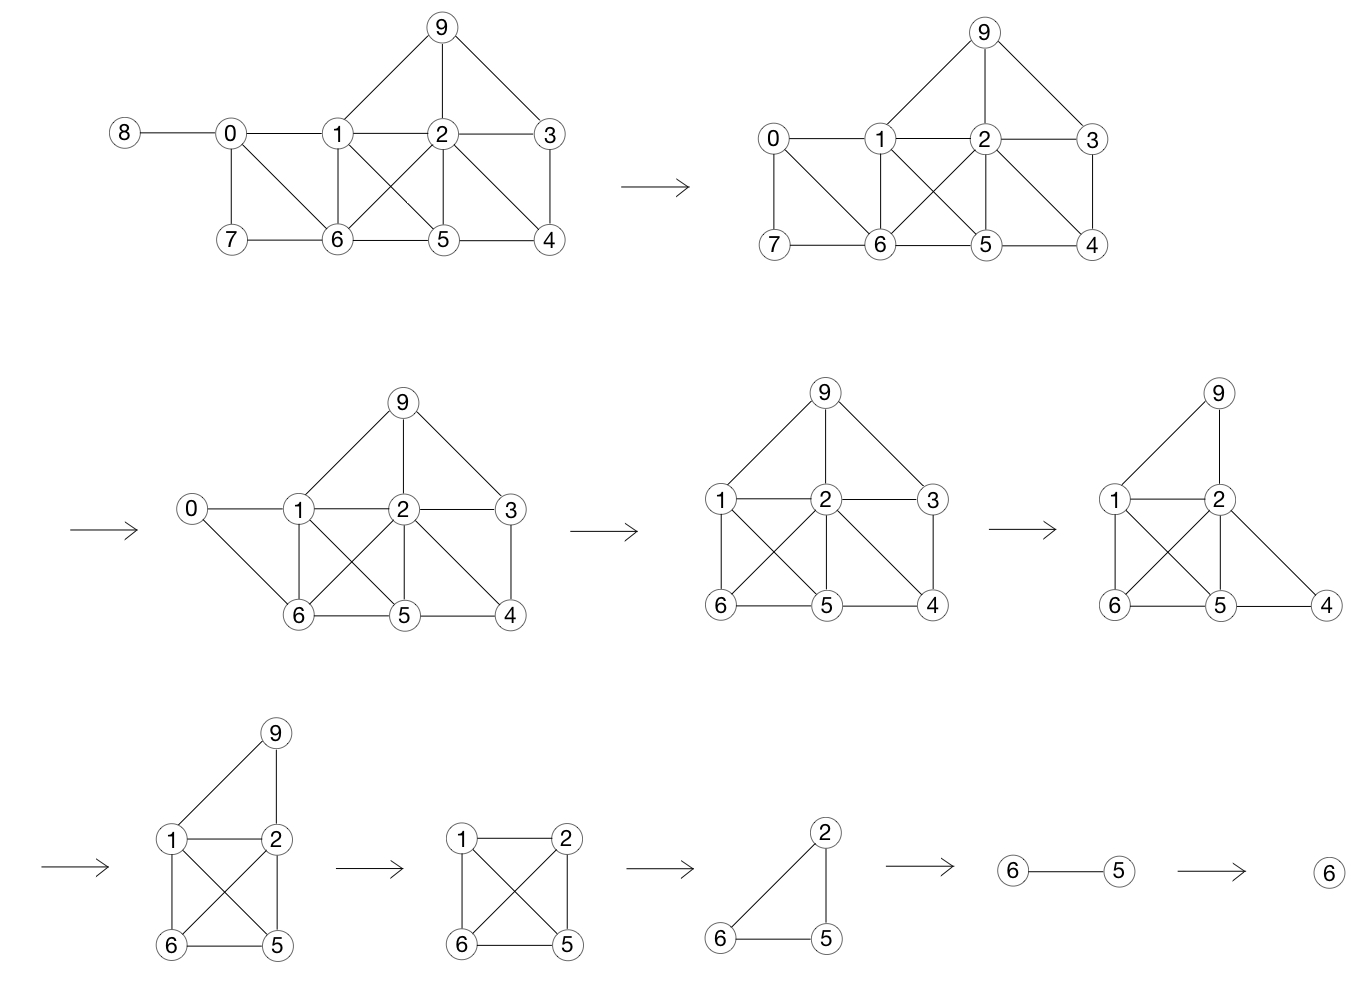
\includegraphics[width=0.9\textwidth]{Ex3.jpeg}
                    \begin{tabular}{|c|c|c|c|c|c|c|c|c|c|c|}
        \hline
            Degrees &0&1& 2&3&2& 2&3& 2& 2&  1\\
            \hline
            Vertex &6&5&2&1&9& 4& 3& 0& 7&   8\\ 
            \hline
        \end{tabular}
    \end{center} 
                The example test result:
            \begin{center}
        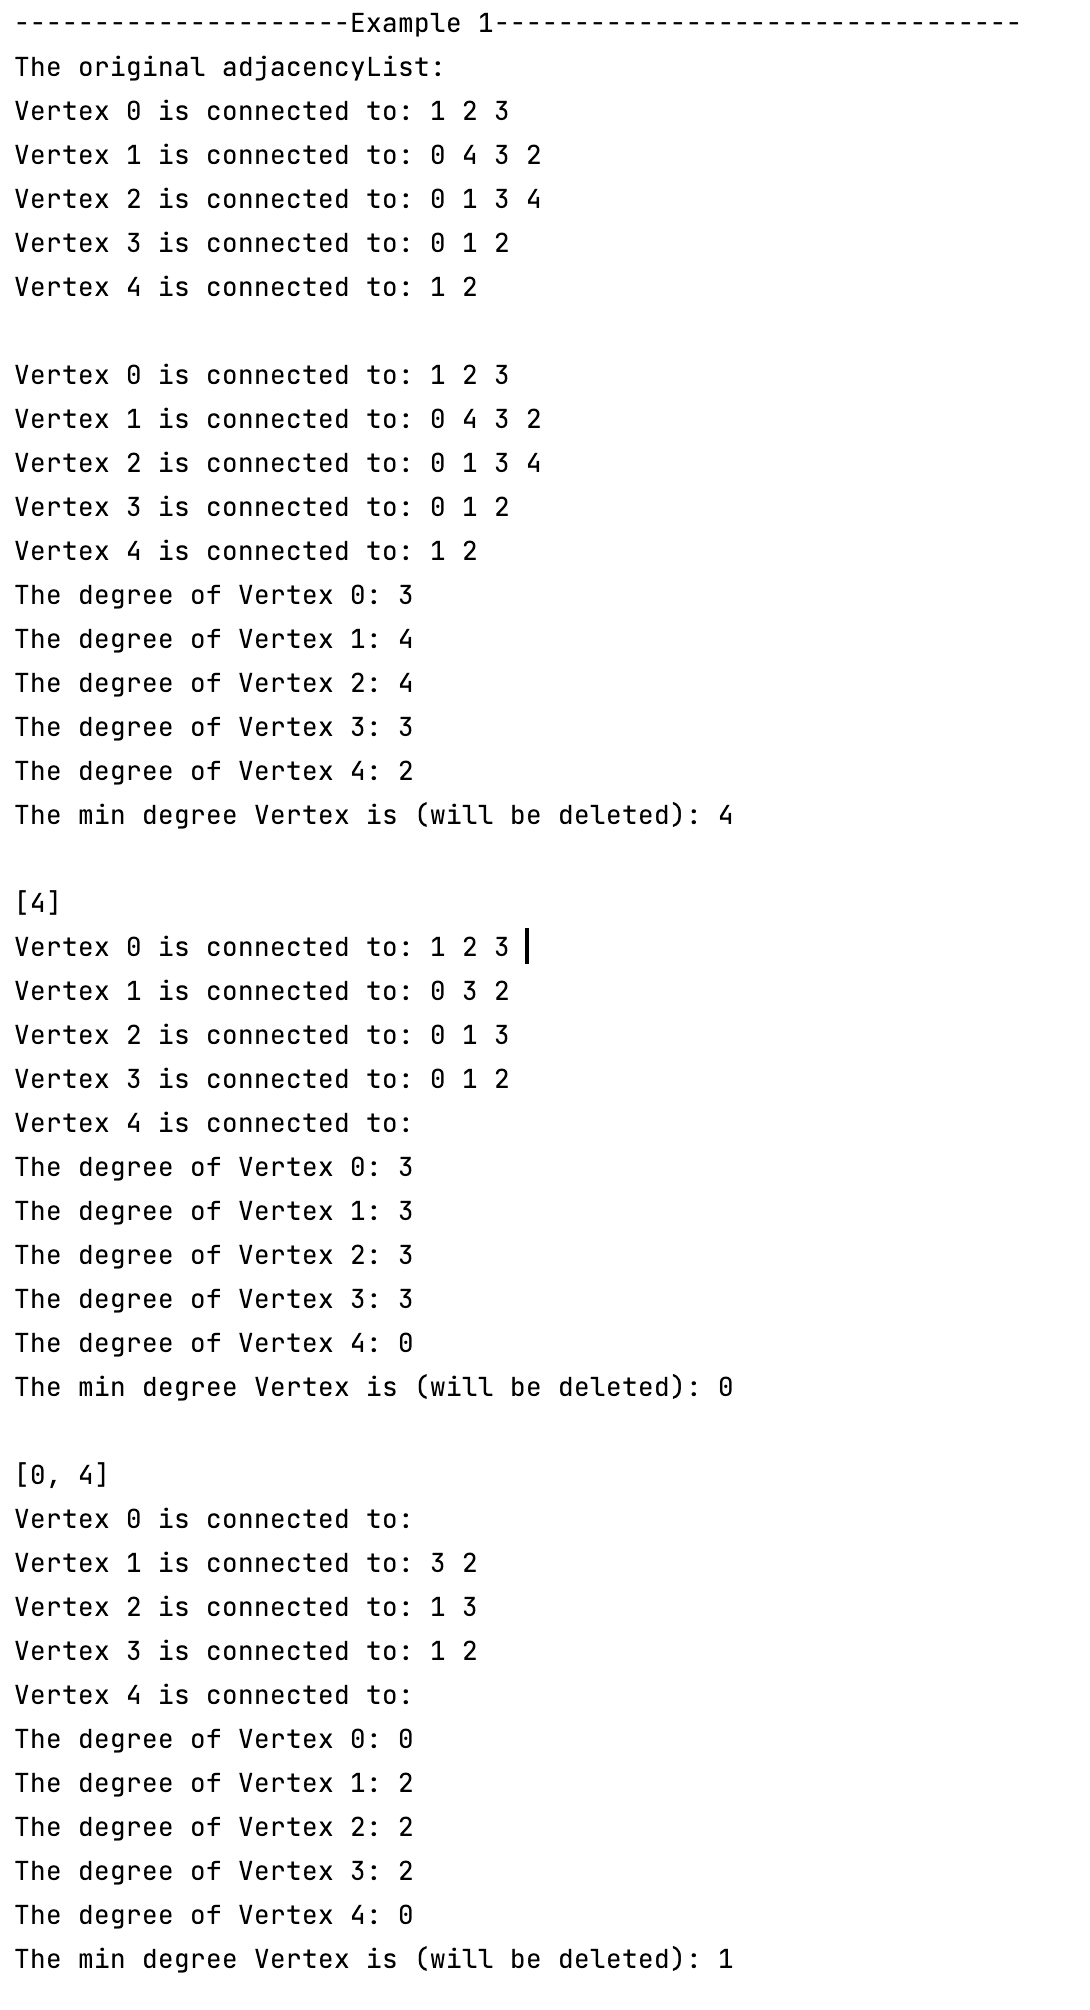
\includegraphics[width=0.6\textwidth]{Ex11.png}
        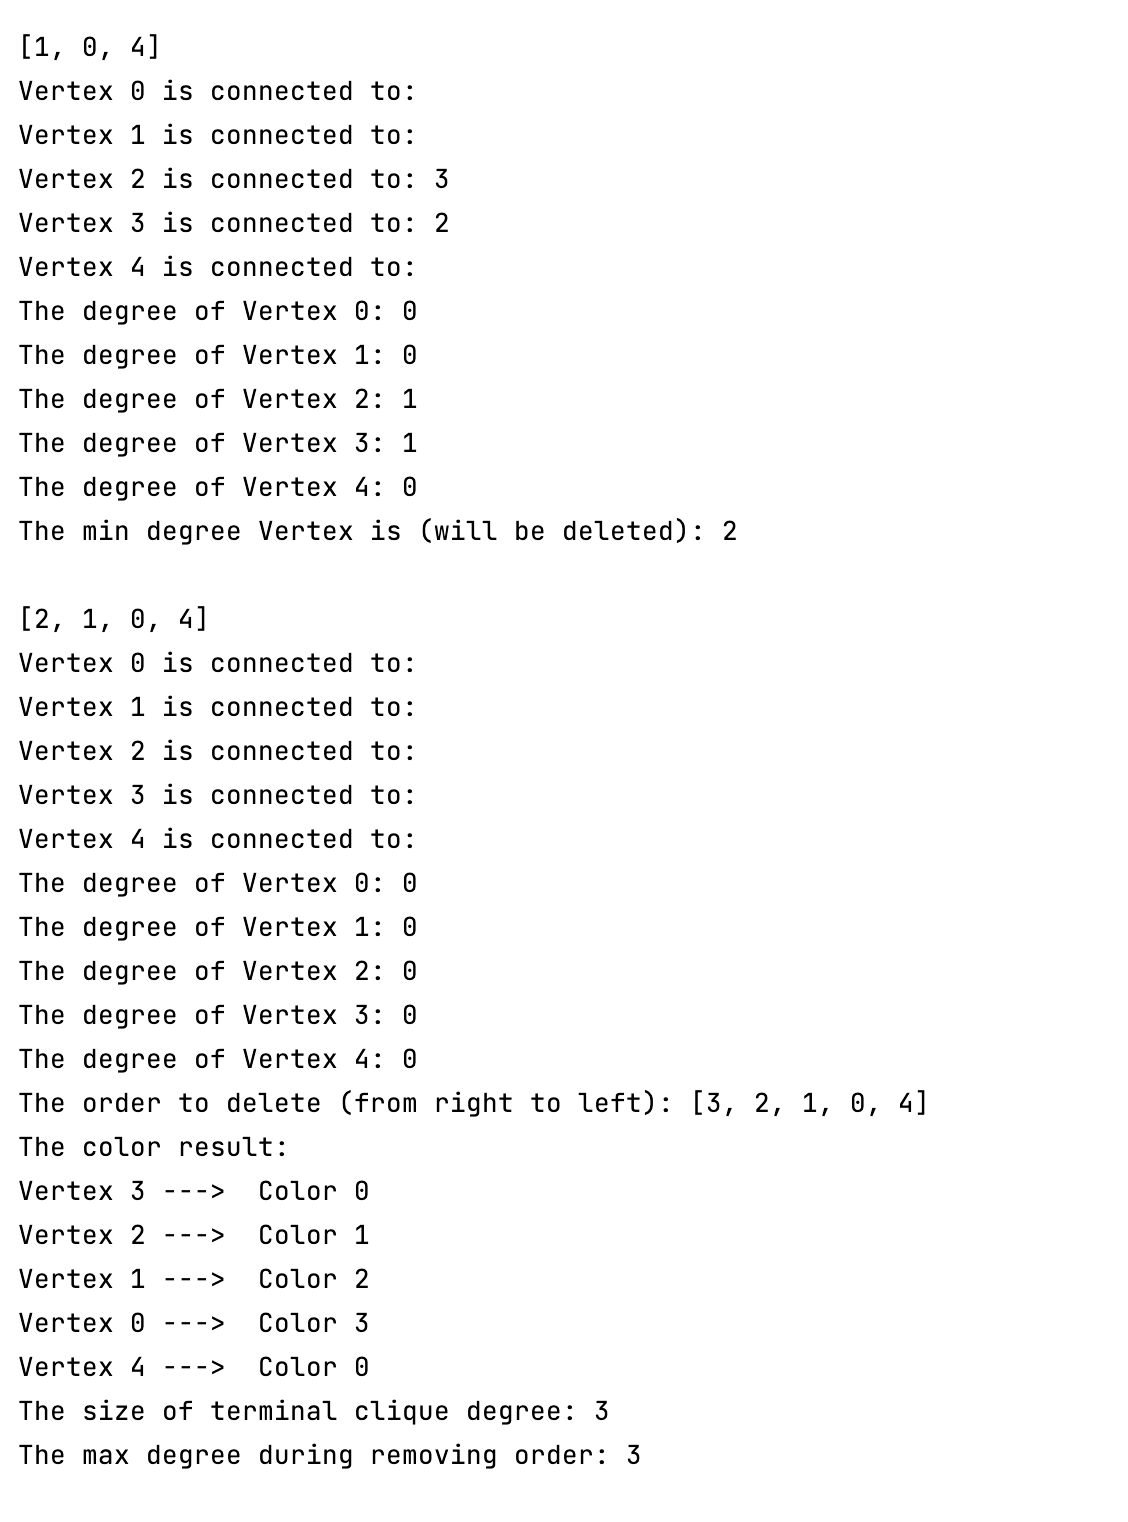
\includegraphics[width=0.6\textwidth]{Ex12.png}
        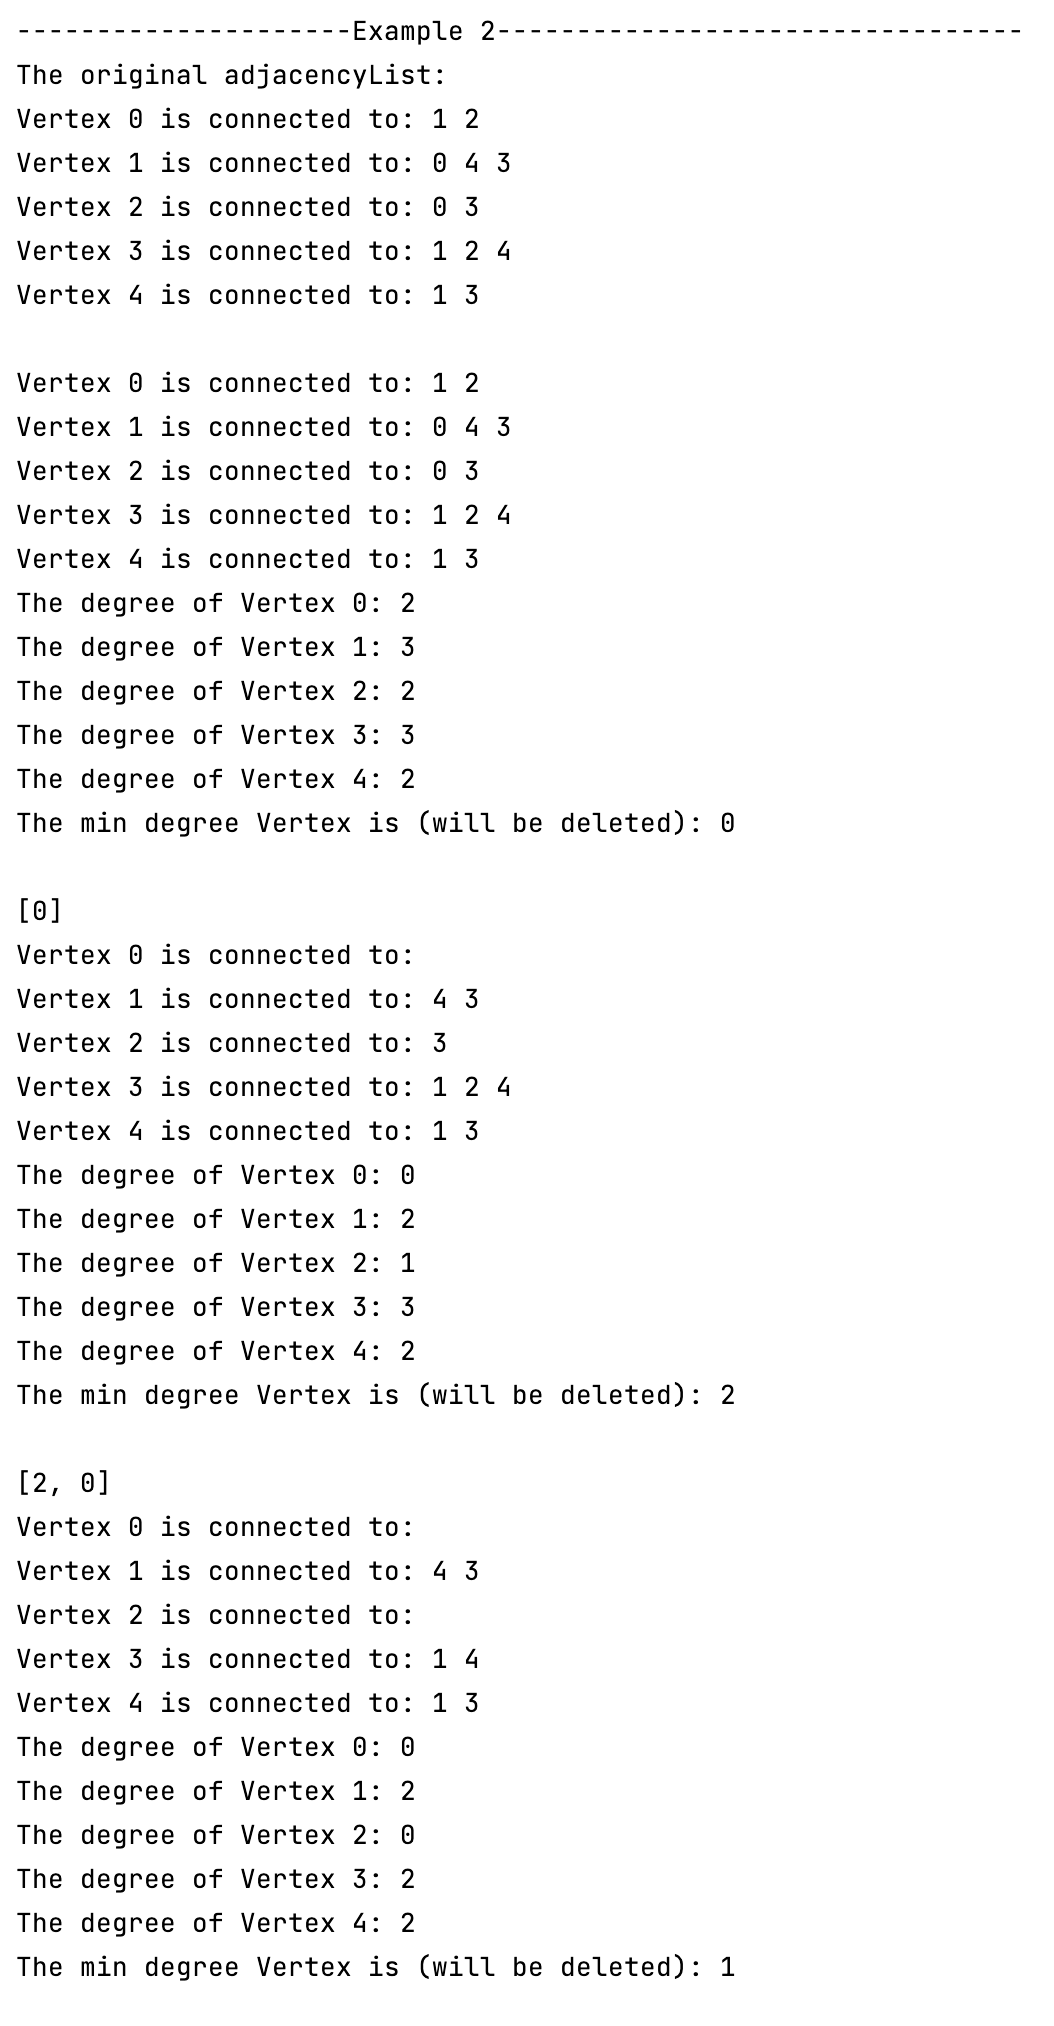
\includegraphics[width=0.6\textwidth]{p25.png}
        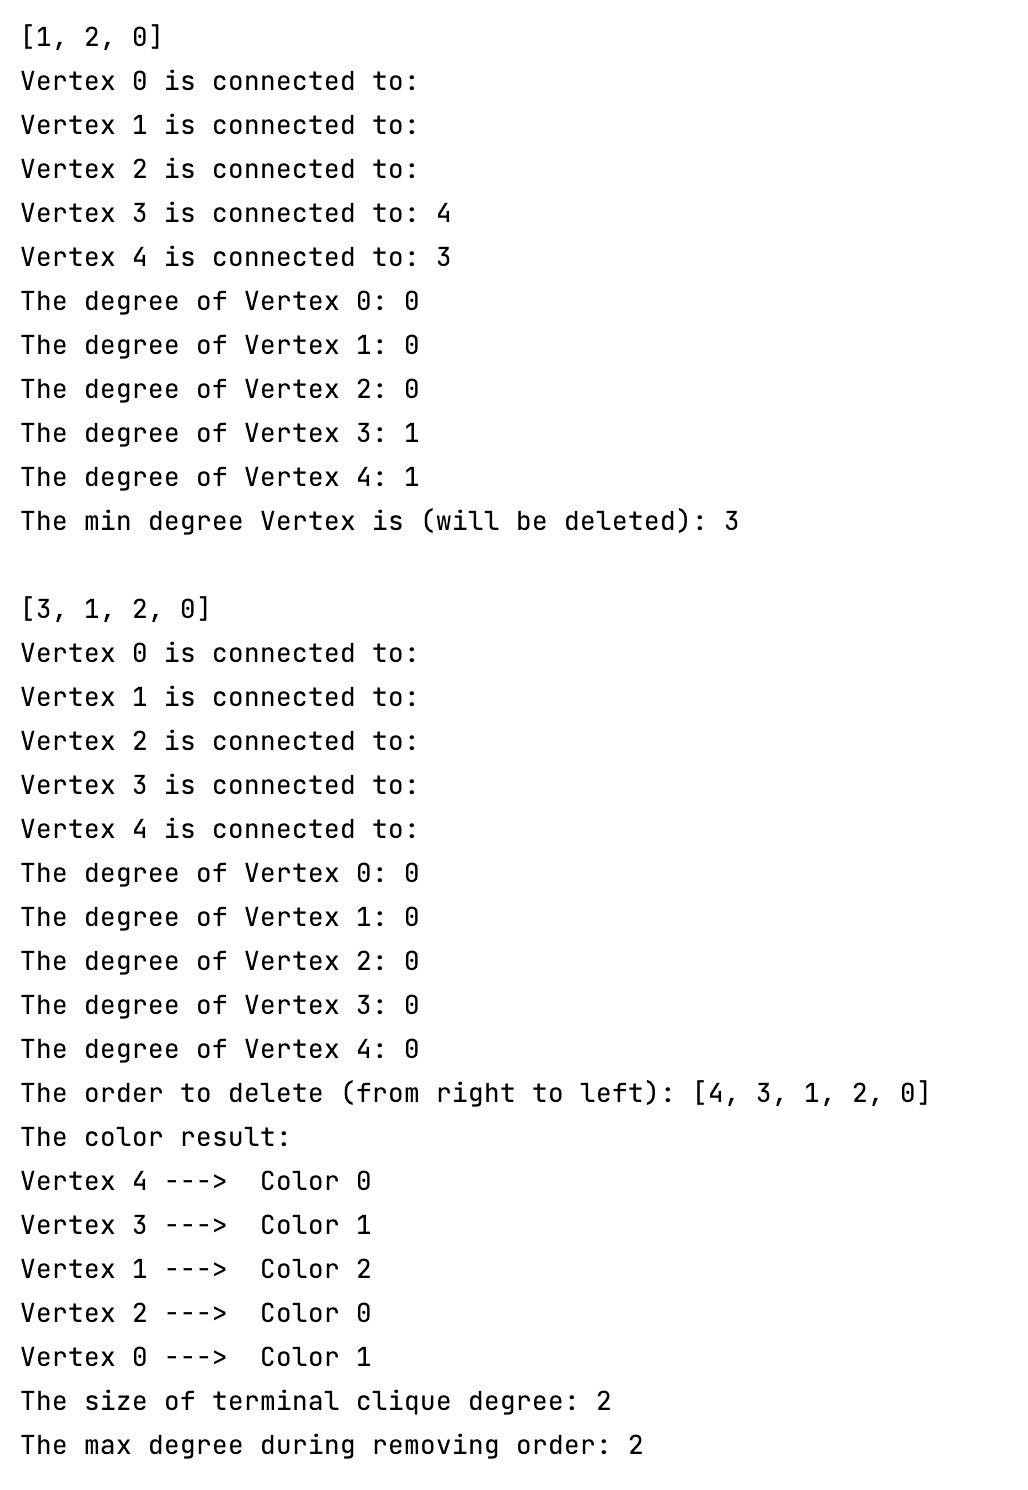
\includegraphics[width=0.6\textwidth]{p26.png}
        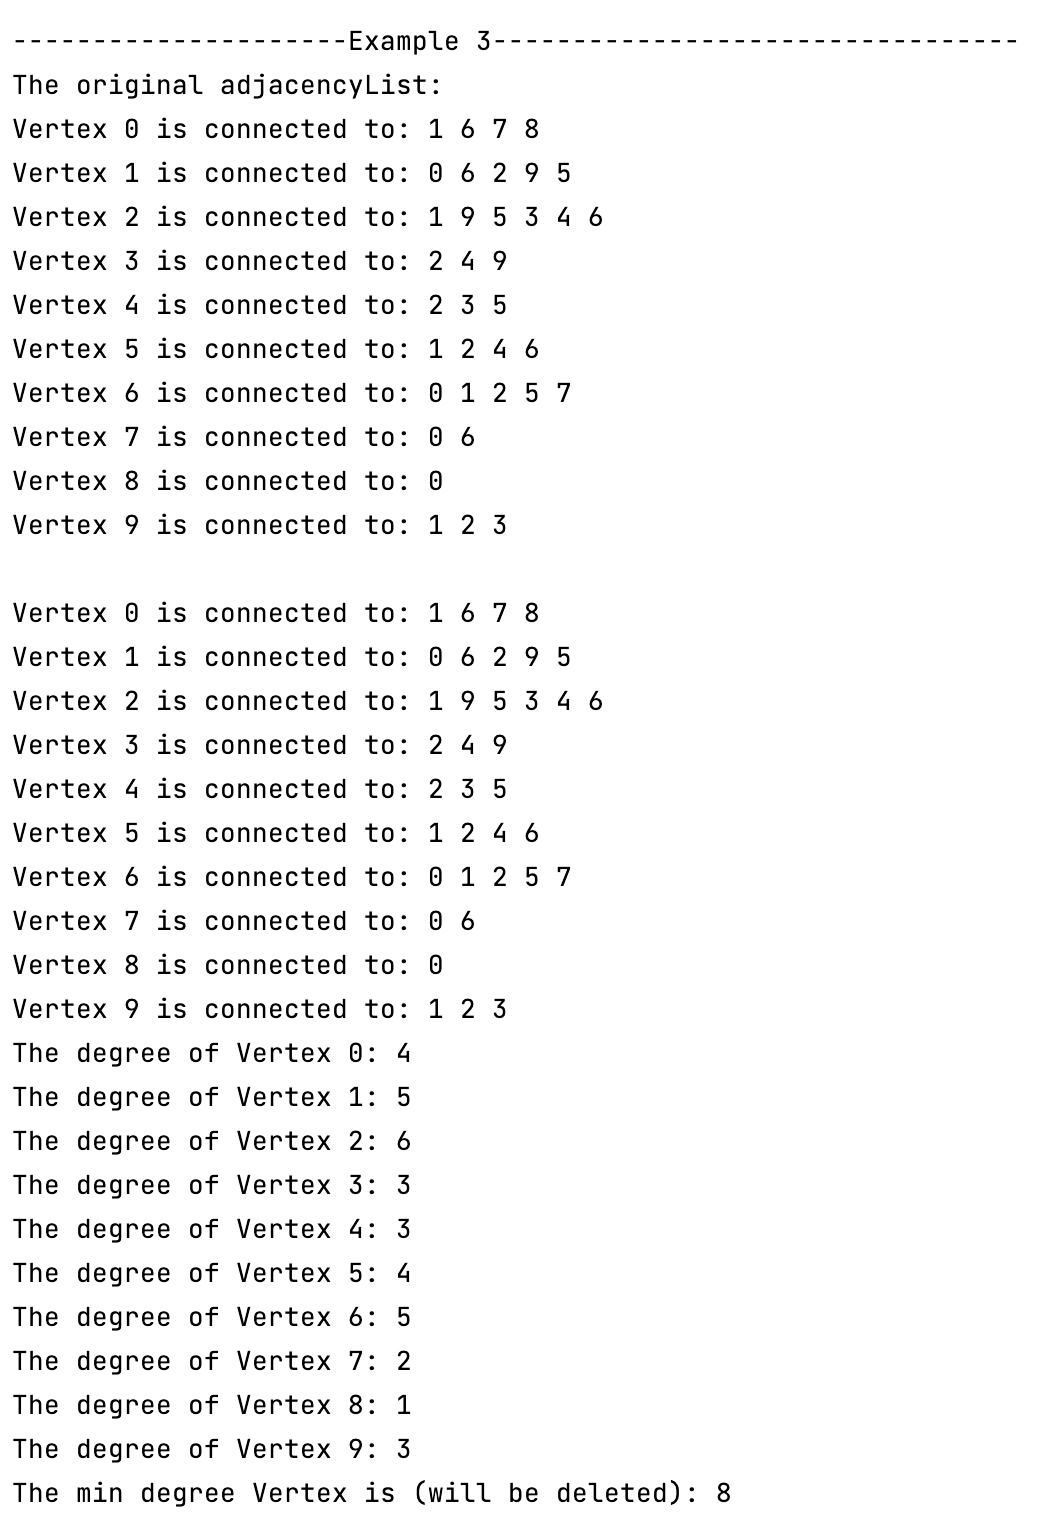
\includegraphics[width=0.6\textwidth]{p27.png}
        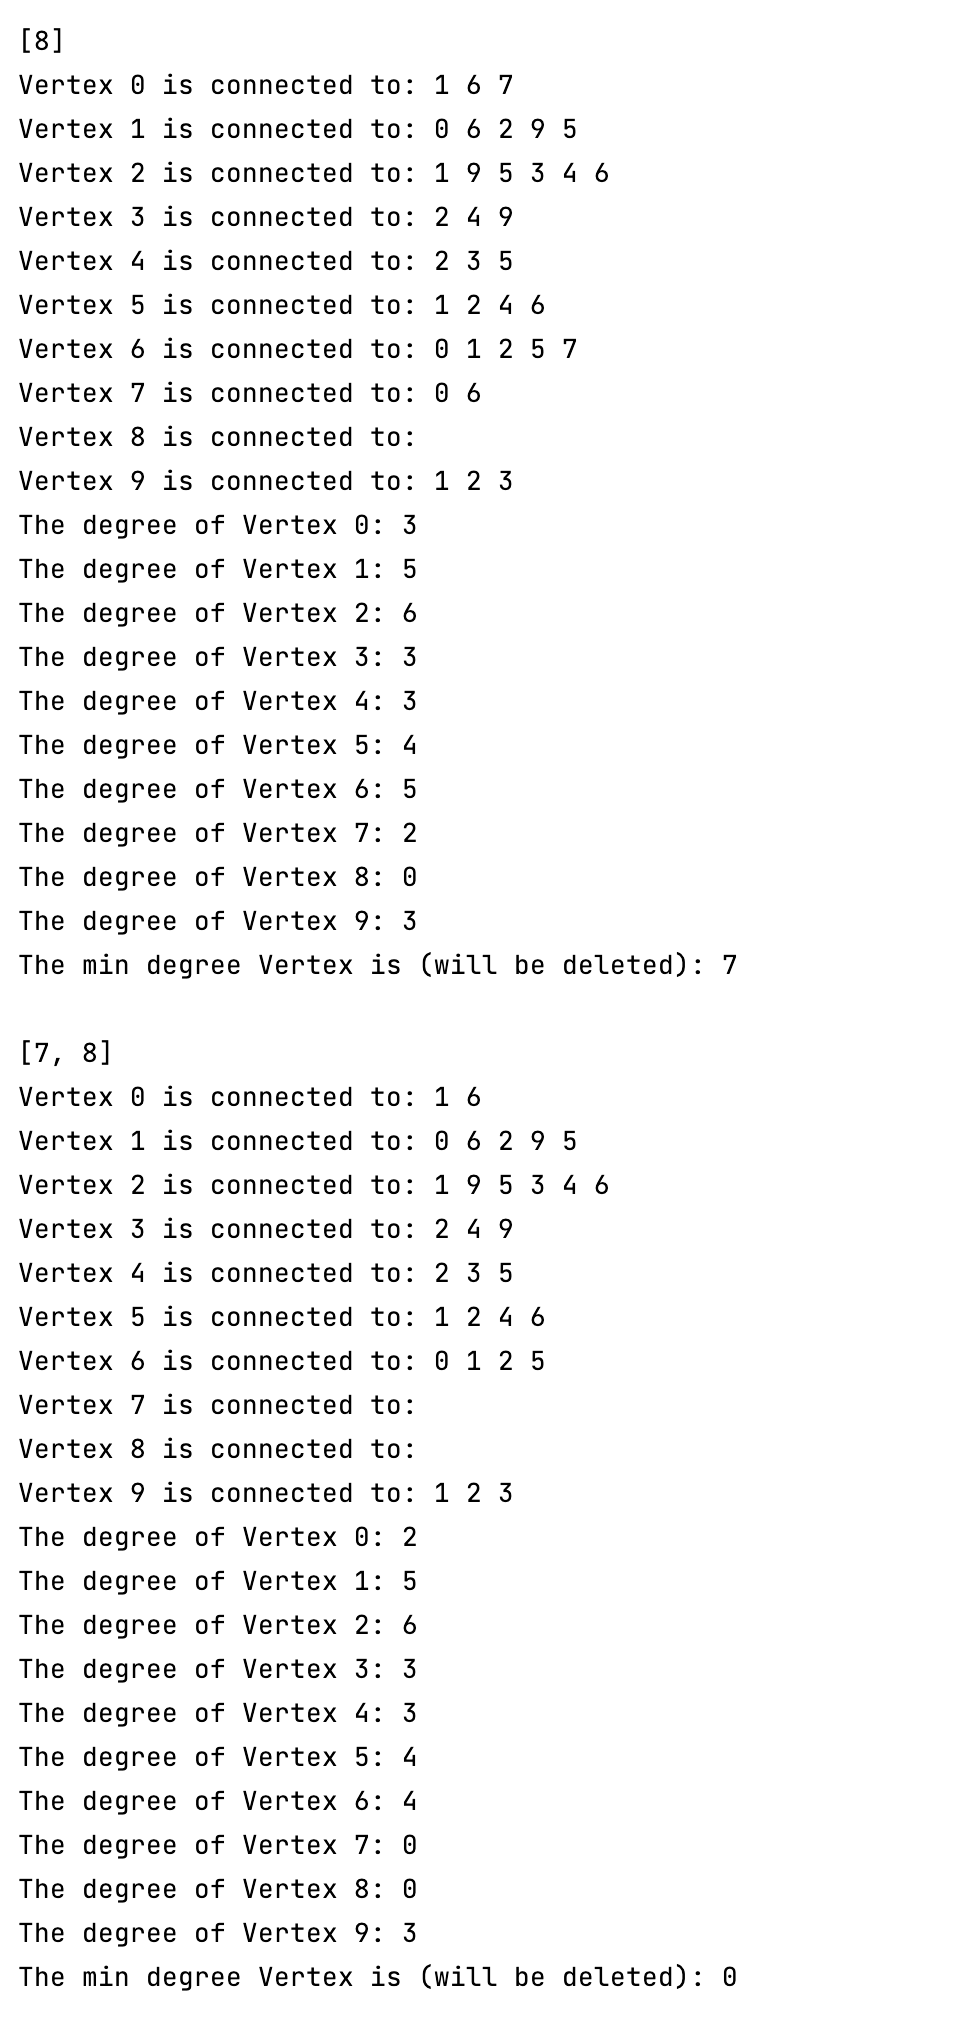
\includegraphics[width=0.6\textwidth]{p28.png}
        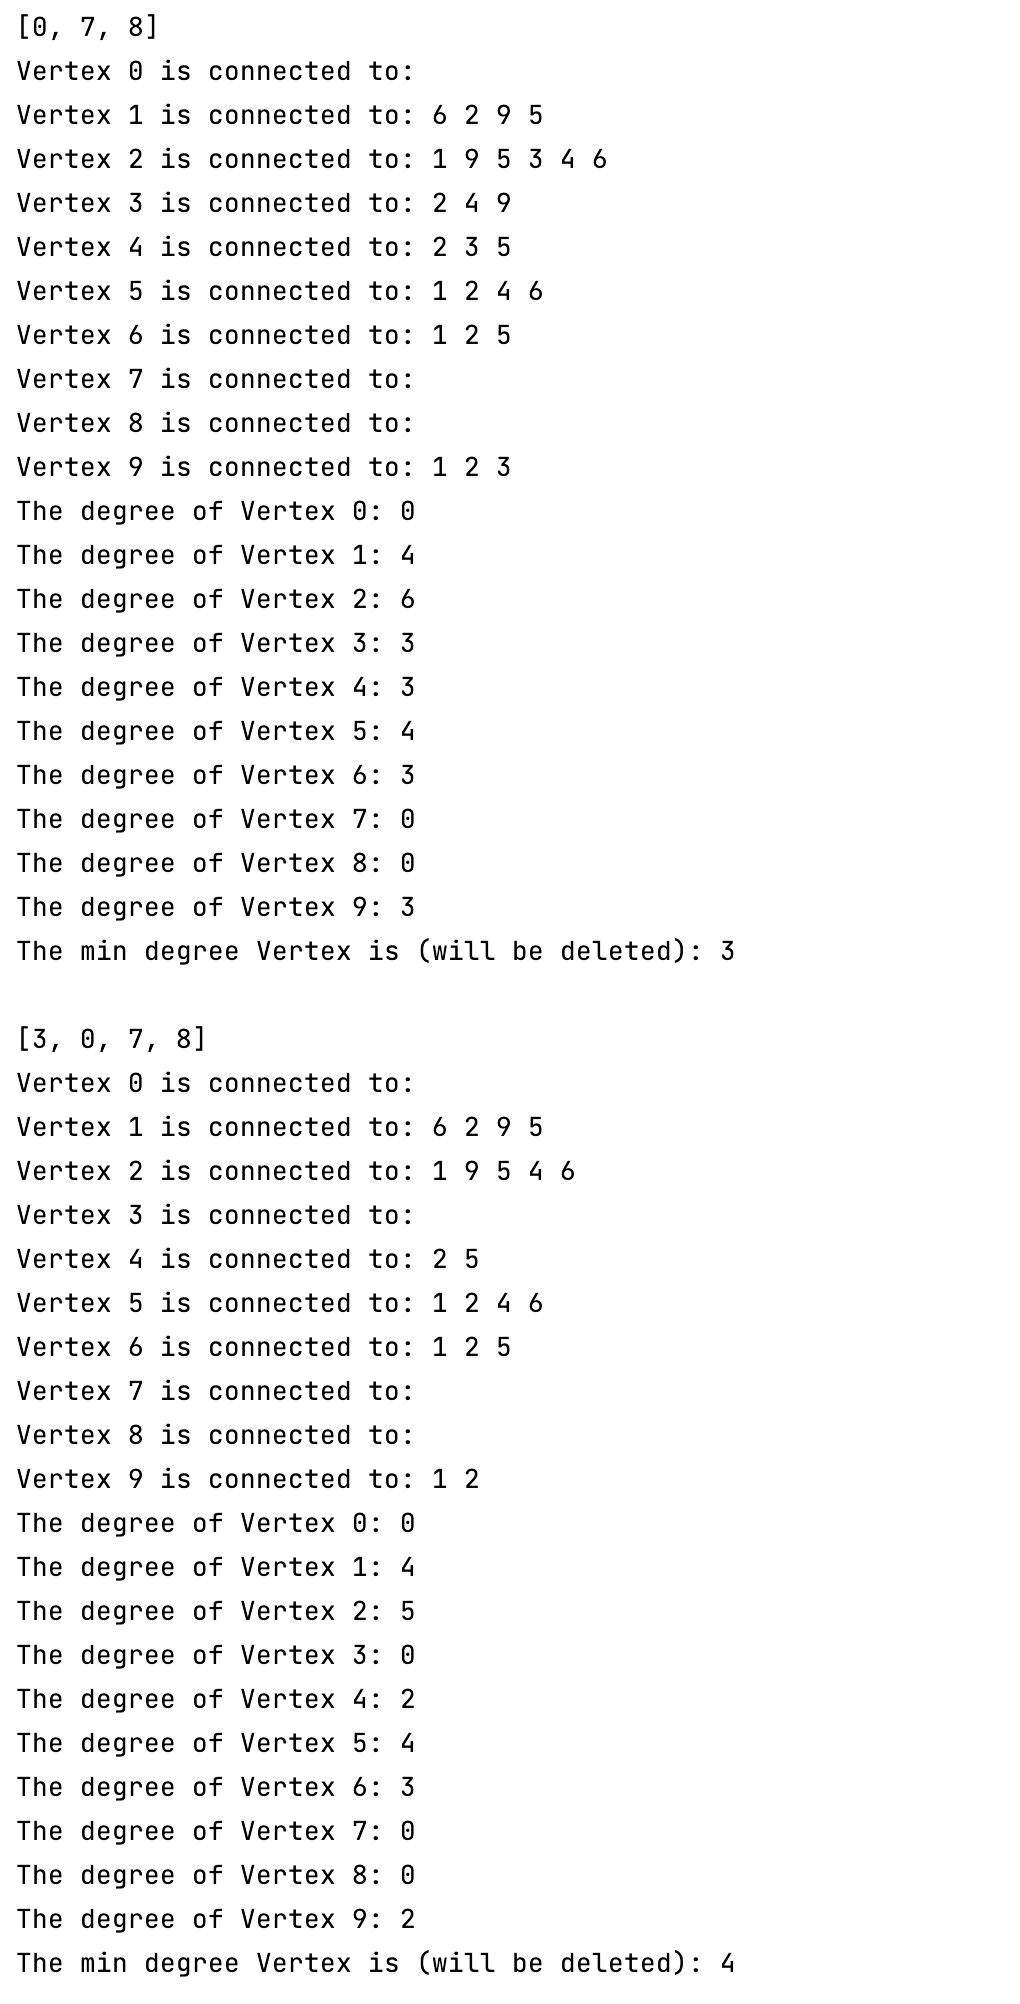
\includegraphics[width=0.6\textwidth]{p29.png}
        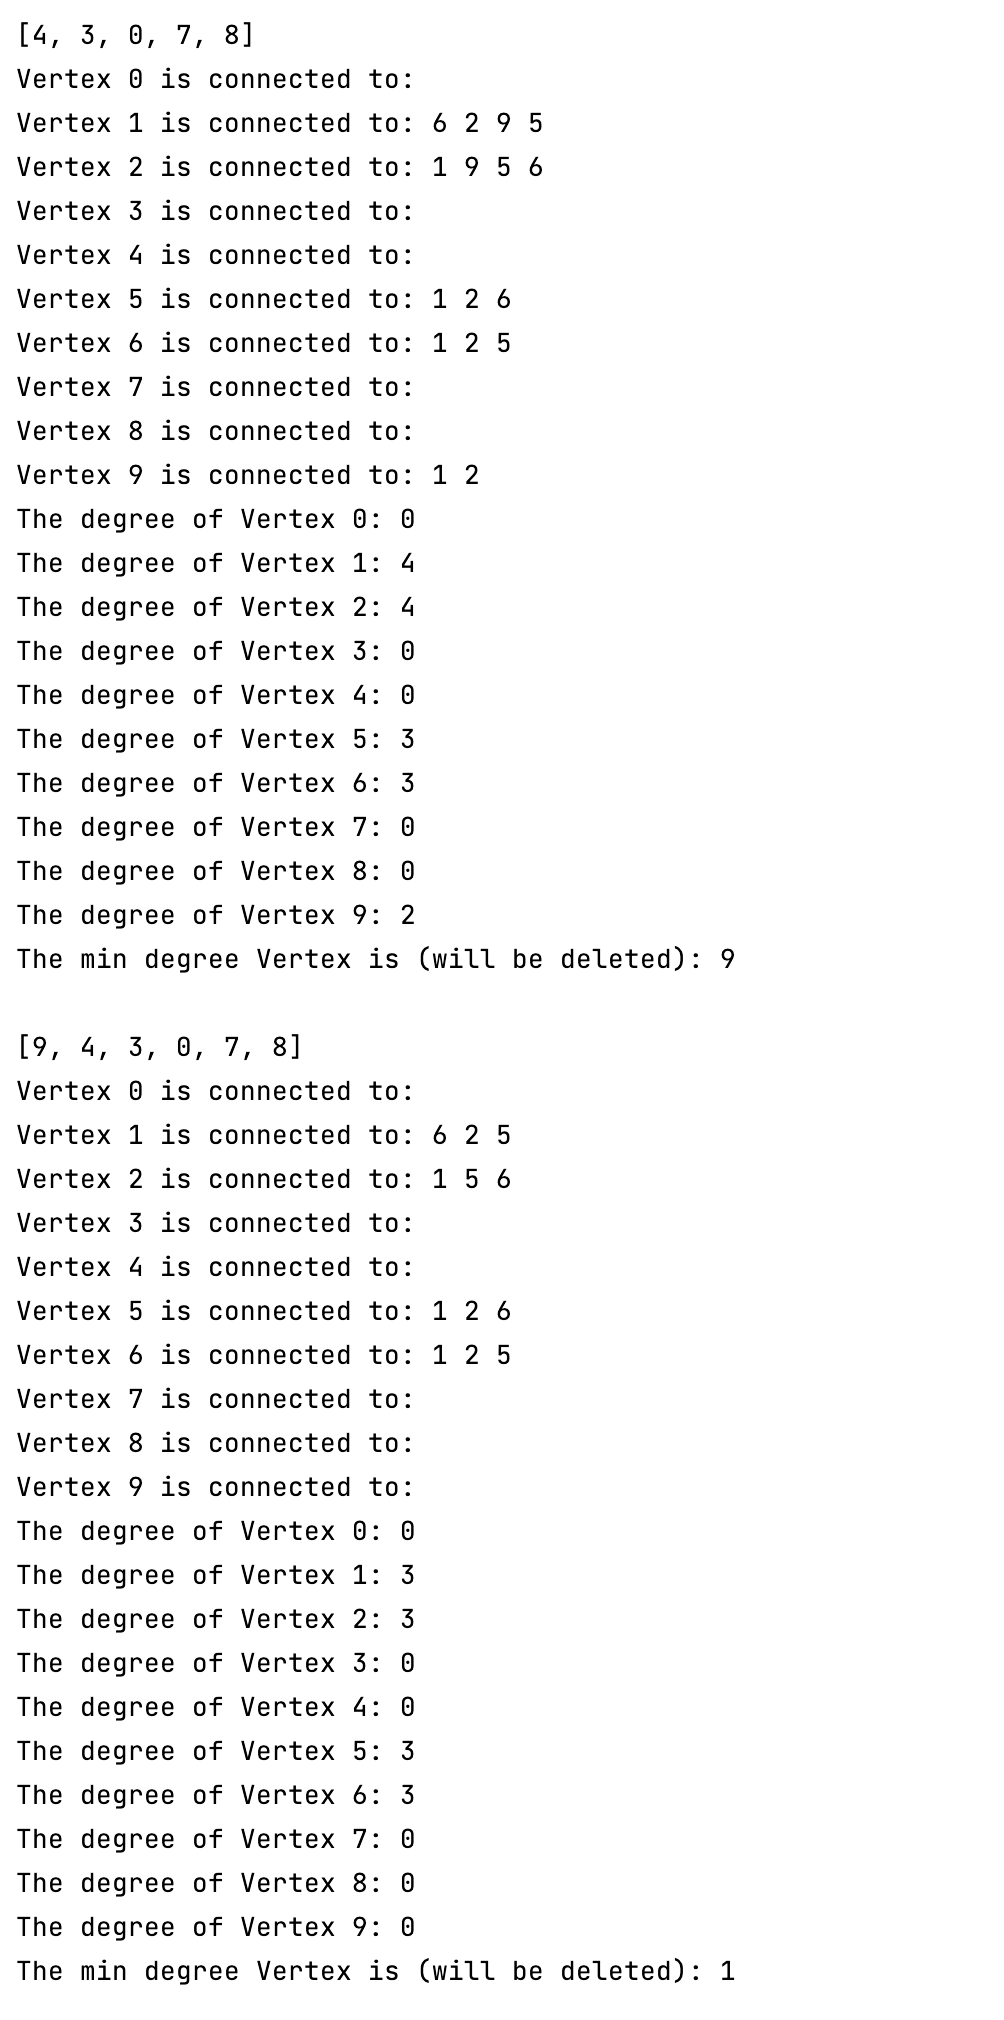
\includegraphics[width=0.6\textwidth]{p30.png}
        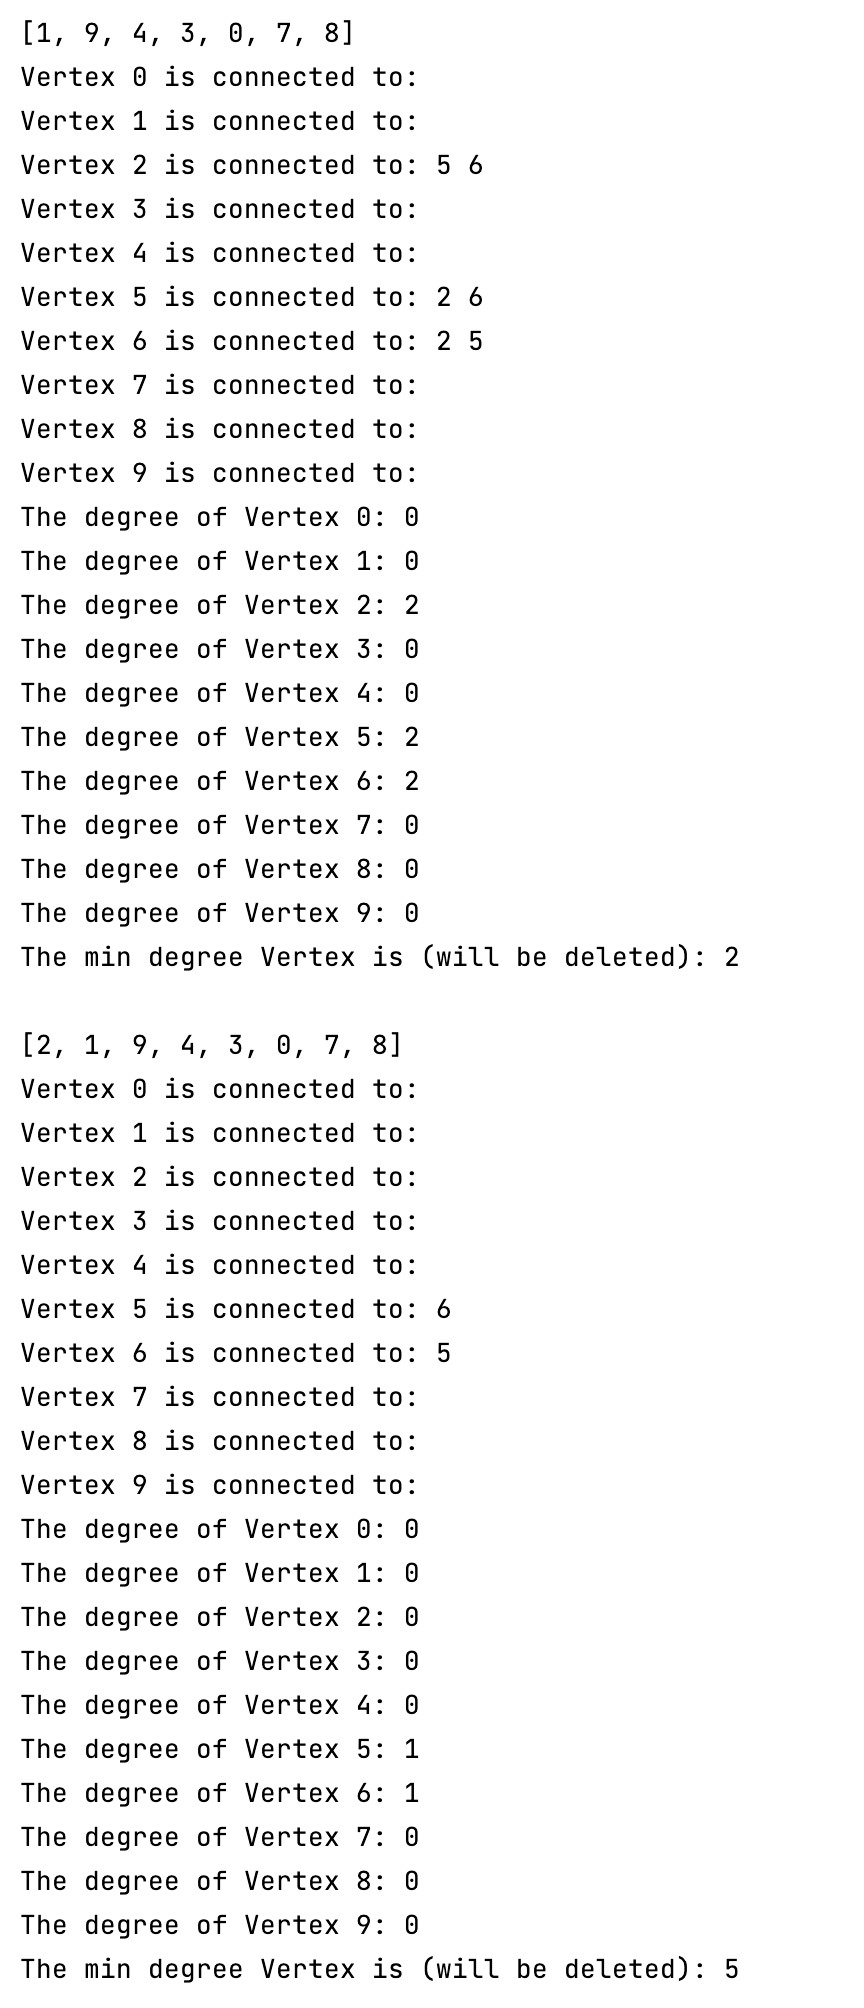
\includegraphics[width=0.5\textwidth]{p31.png}
        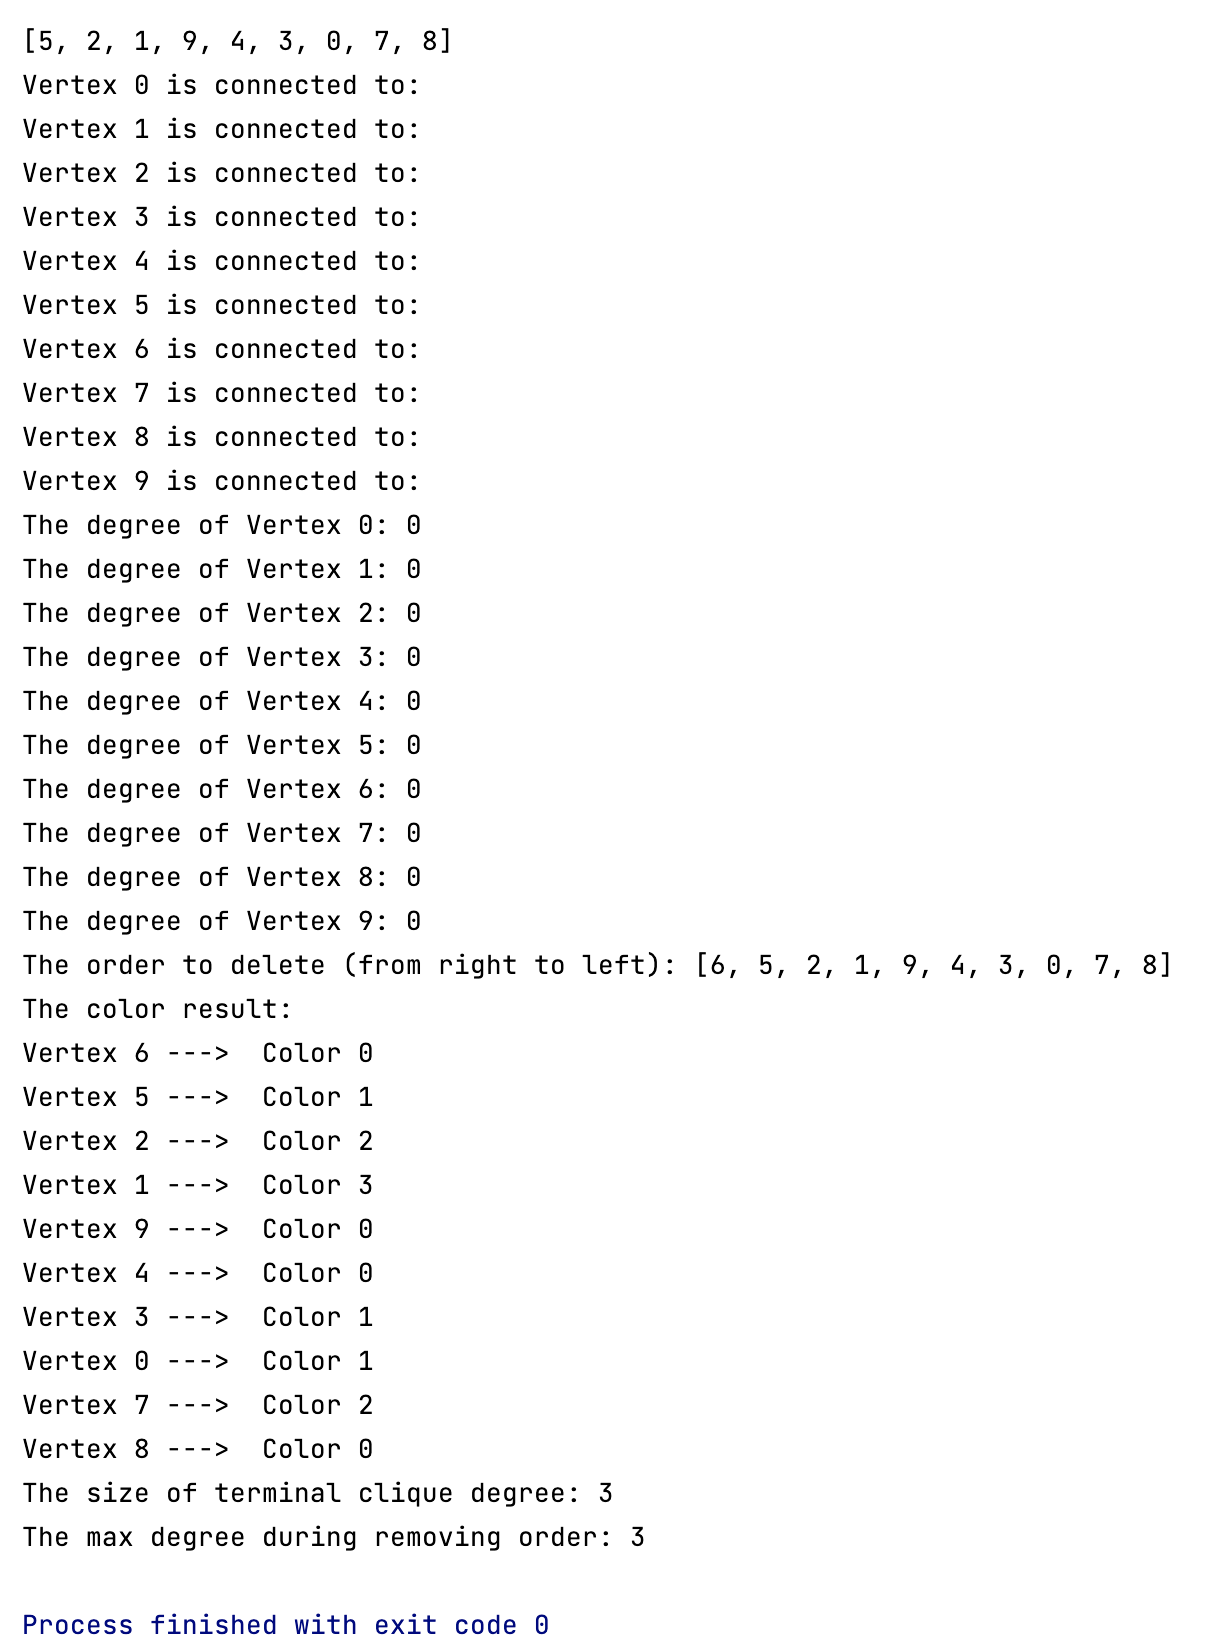
\includegraphics[width=0.7\textwidth]{p32.png}
    \end{center}
    
\item Smallest Original Degree Last (SODL) Ordering: This algorithm is similar to the Smallest Last Vertex (SLV) ordering, but instead of using the current degree during the algorithm's execution, it considers the original degree of each vertex. The vertex with the smallest original degree is placed last, and the process is repeated for the remaining vertices. The Smallest Original Degree Last method is a subset of the smallest last ordering. Should determine the vertices to color based on their original degree, but not remove them from graph. This should run in $\Theta(V+E)$.

    \begin{minted}
[frame=lines,framesep=2mm,baselinestretch=1.2,fontsize=\footnotesize,linenos]{java}
// Method 2: Smallest Original Degree Last (SODL) Ordering:
    public static int findMaxDegreeVertex(ArrayList<ArrayList<Integer>> am, ArrayList<Integer> exit){
        int maxDegree = Integer.MIN_VALUE;
        int maxDegreeVertex = -1;

        for (int i = 0; i < am.size(); i++){
            int degree = am.get(i).size();

            System.out.println("The degree of Vertex " + i + ": " + degree);
            if (degree > maxDegree && degree > 0 && !exit.contains(i)){
                maxDegree = degree;
                maxDegreeVertex = i;
            }
        }

        return maxDegreeVertex;
    }


    private static ArrayList<Integer> smallestOriginalDegreeLast(ArrayList<ArrayList<Integer>> am){
        ArrayList<Integer> solOrder = new ArrayList<>();
        int V = am.size();
        System.out.println(V);


        while(solOrder.size() < am.size()){
            int minDegreeVertex = findMaxDegreeVertex(am, solOrder);

            System.out.println("The vertex add to solOrder "+ minDegreeVertex);

            solOrder.add(0, minDegreeVertex);

        }

        System.out.println("smallest orginal degree Last(from right to left) " + solOrder);

        return solOrder;
    }

    \end{minted}
            The example test result:
            \begin{center}
        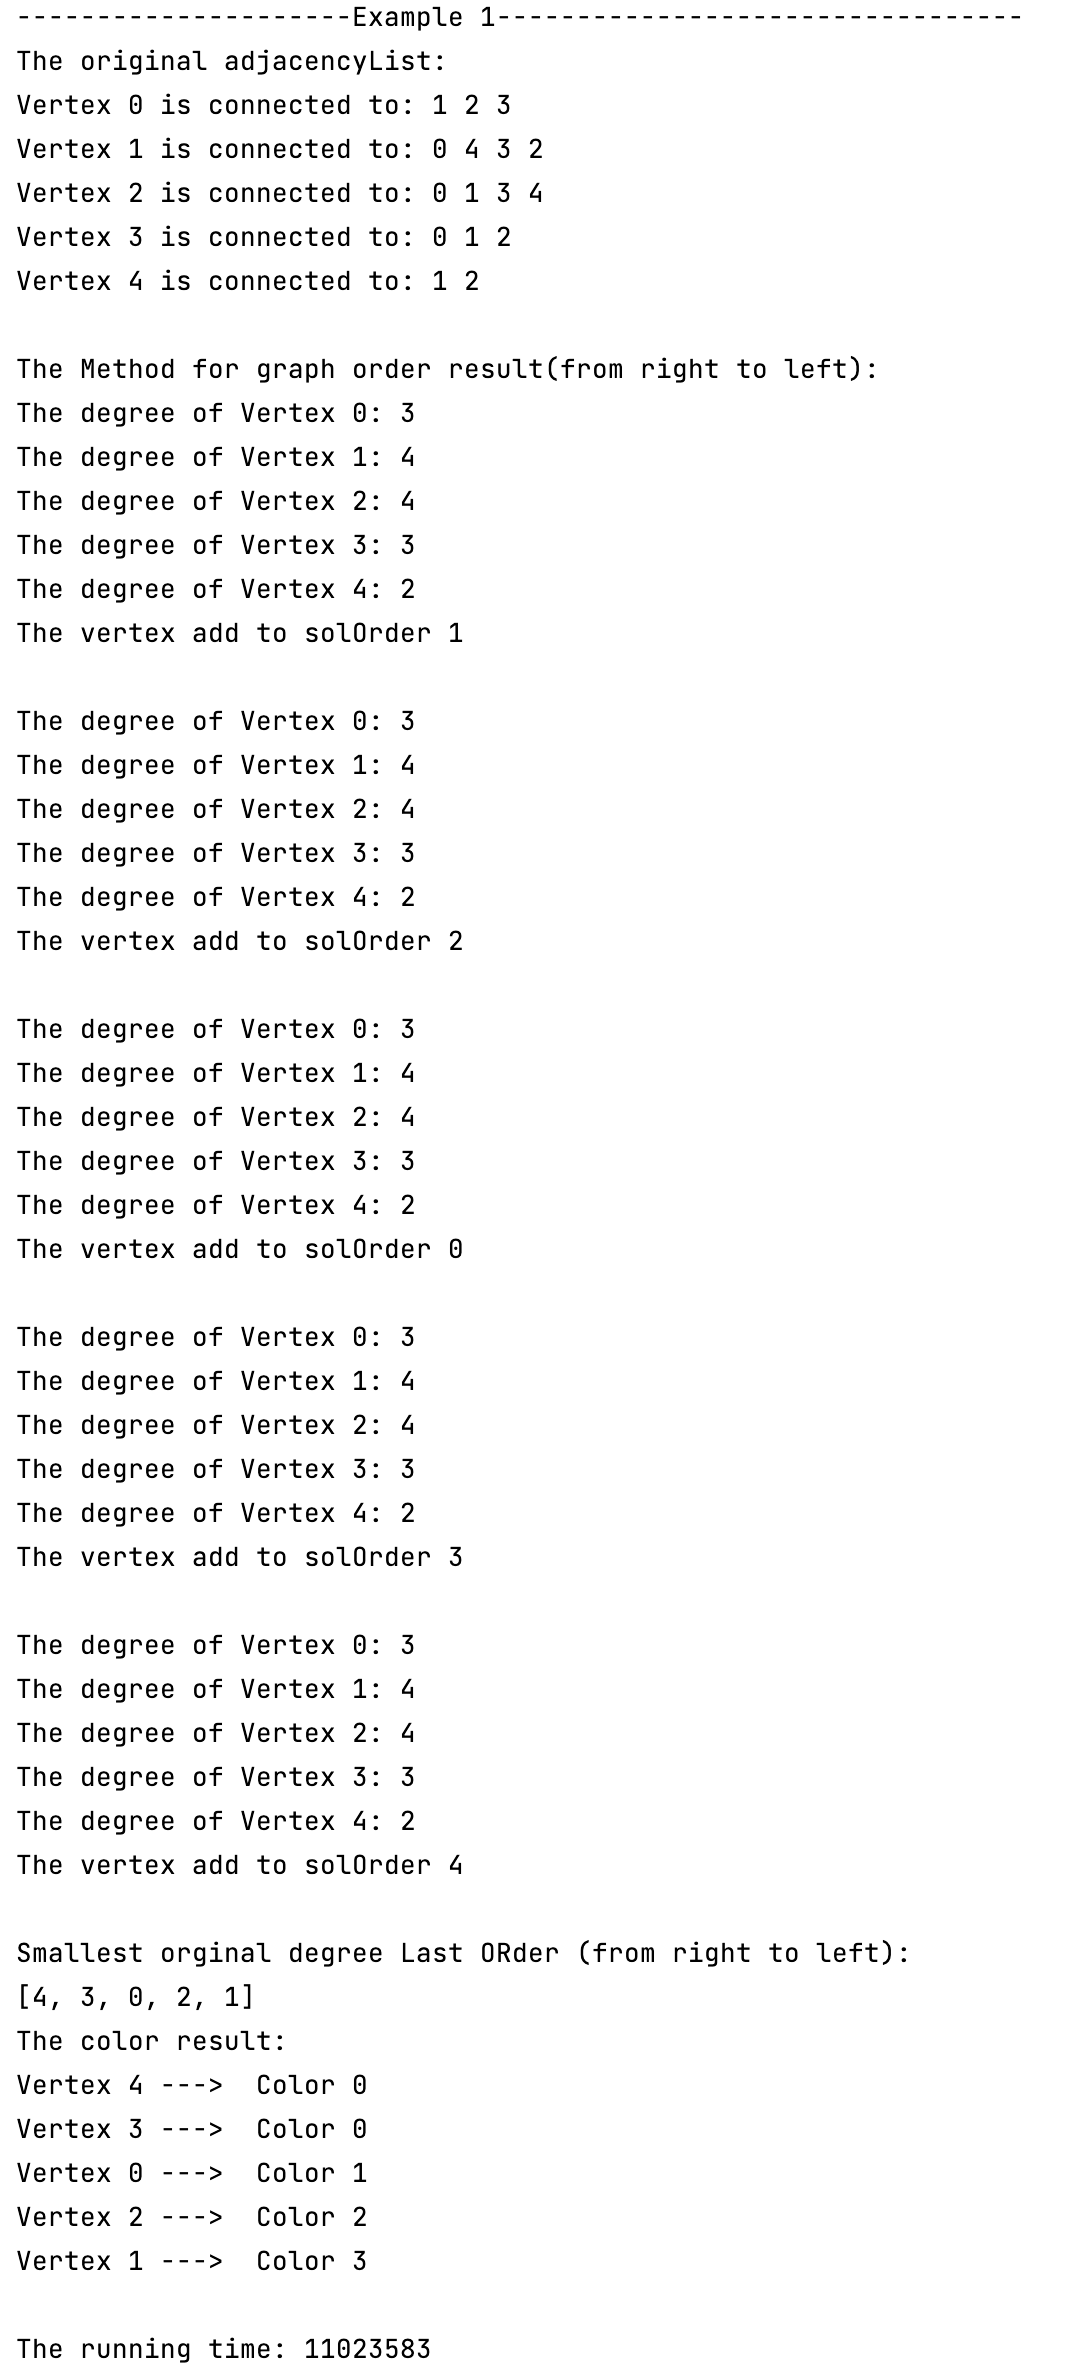
\includegraphics[width=0.6\textwidth]{p18.png}
        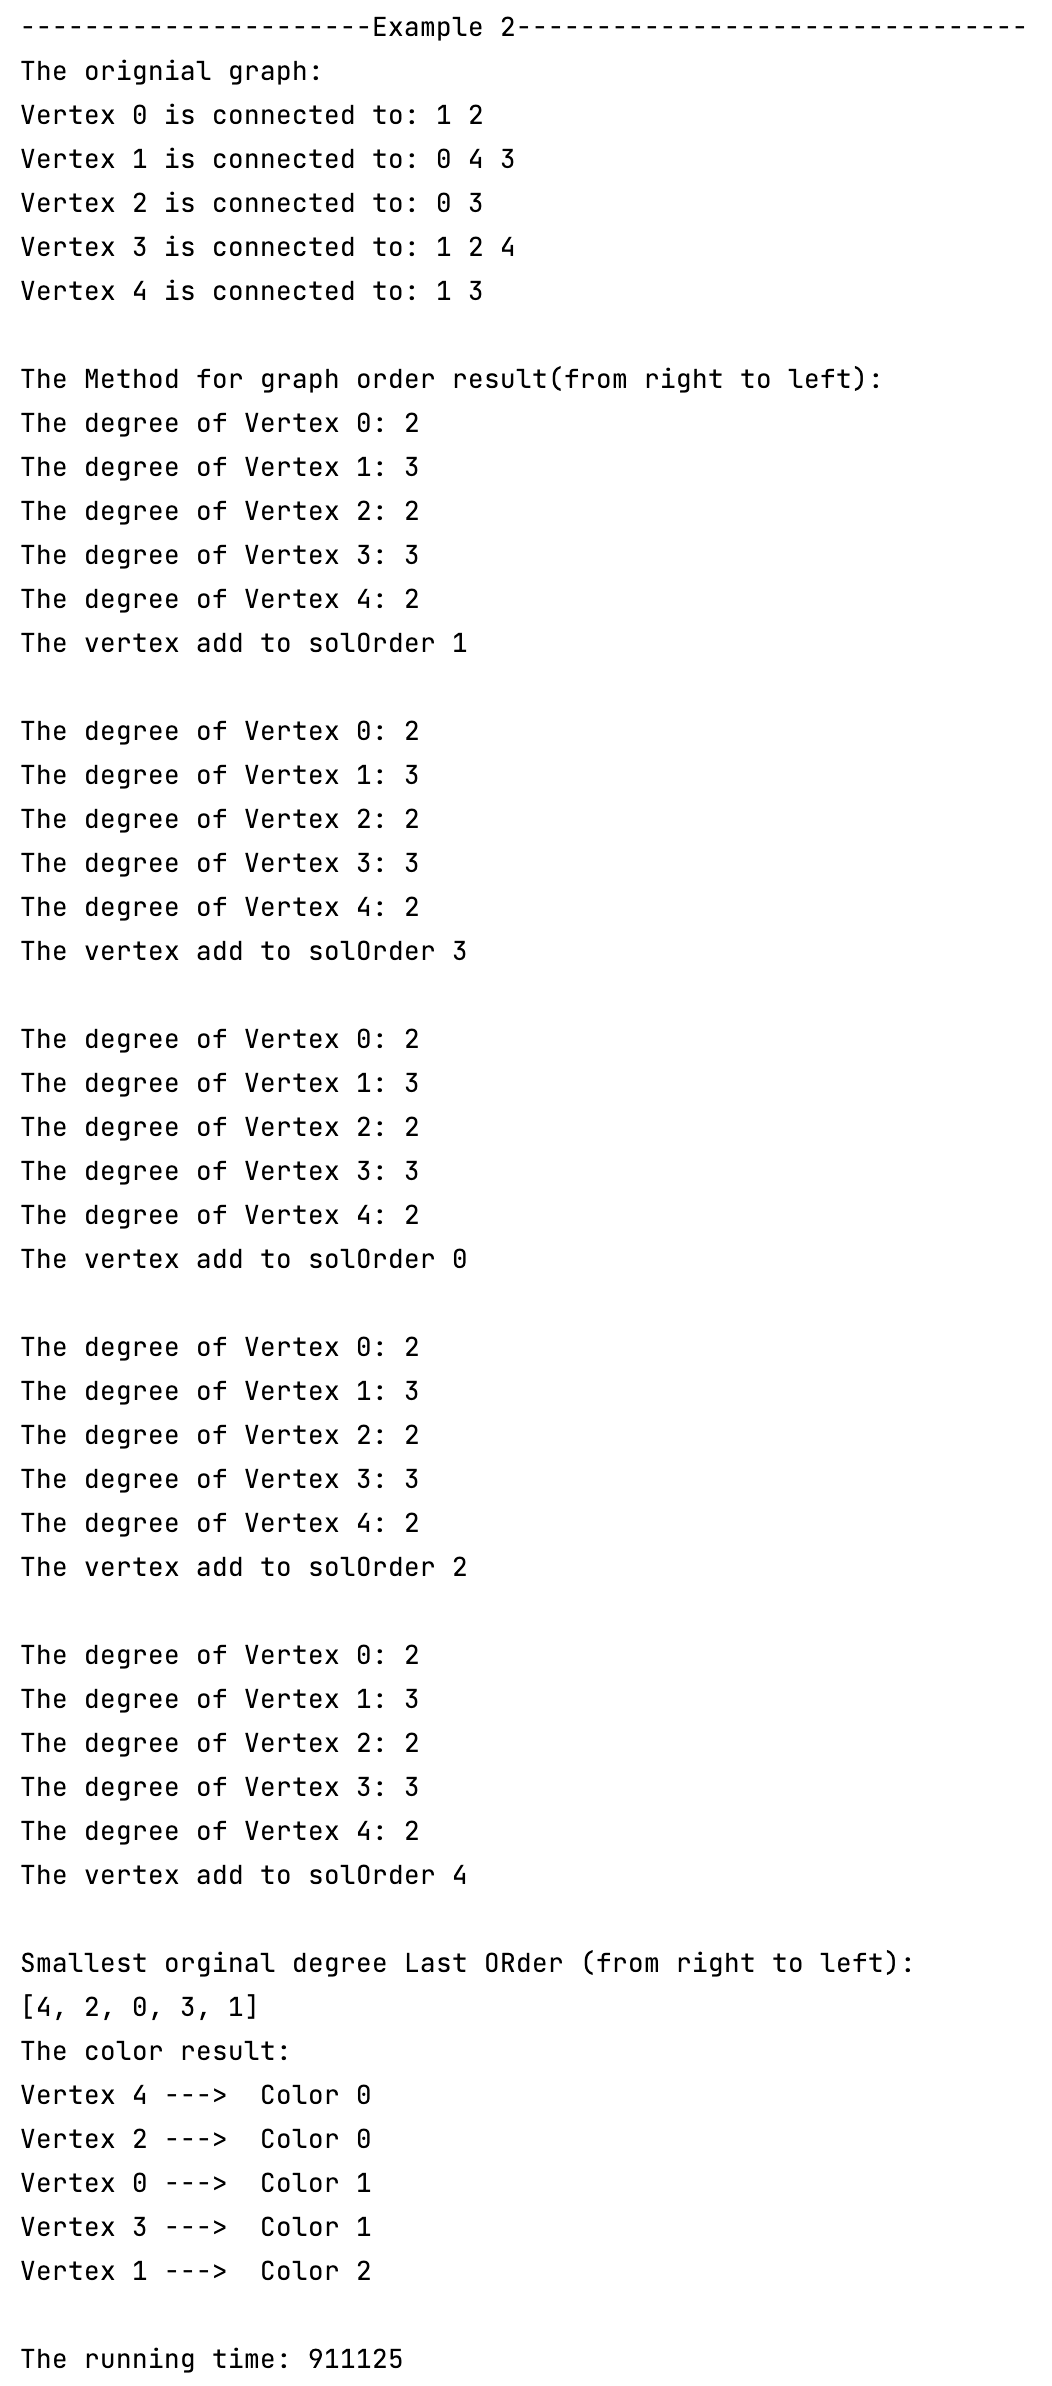
\includegraphics[width=0.6\textwidth]{p19.png}
        \includegraphics[width=0.6\textwidth]{p20.png}
        \includegraphics[width=0.6\textwidth]{p21.png}
        \includegraphics[width=0.6\textwidth]{p22.png}
    \end{center}


\item Uniform Random Ordering: As the name suggests, this algorithm generates a random ordering of the vertices in the graph. This can be useful in certain heuristics or sampling techniques where multiple random orderings are tested to find a suitable solution. It can be implemented simply by shuffling the array of vertex indices.
    \begin{minted}[frame=lines,framesep=2mm,baselinestretch=1.2,fontsize=\footnotesize,linenos]{java}
    // Method 3: Uniform Random Ordering:
    public static ArrayList<Integer> uniformrandom(ArrayList<ArrayList<Integer>> am){
        ArrayList<Integer> unOrder = new ArrayList<Integer>();
        for (int i = 0; i < am.size(); i++){
            unOrder.add(i);
        }

        Collections.shuffle(unOrder,new Random());
        // the list to be shuffled
        // the source of randomness to use to shuffle the list.


        System.out.println(unOrder);


        return unOrder;
    }
    \end{minted}
        The example test result:
            \begin{center}
        \includegraphics[width=0.6\textwidth]{p15.png}
        \includegraphics[width=0.6\textwidth]{p16.png}
        \includegraphics[width=0.6\textwidth]{p17.png}
    \end{center}


\item Breadth-First Search (BFS) Ordering: This algorithm traverses the graph in a breadth-first manner, exploring all the neighbors of a vertex before moving on to their neighbors. The order in which the vertices are visited during the traversal is the BFS ordering. BFS is used in various graph search algorithms, pathfinding, and connectivity testing.\cite{BFS}
\begin{enumerate}
    \item Let G = (V, E) be a graph with vertex set V and edge set E.
\item Choose a starting vertex s in V.
\item Initialize a queue Q and a list P (to store the BFS ordering).
\item Mark vertex s as visited and enqueue it into Q.
\item While Q is not empty:
\begin{enumerate}
    \item Dequeue a vertex v from Q and add it to the BFS ordering list P.
    \item For each unvisited neighbor w of vertex v: Mark w as visited and enqueue it into Q.
\end{enumerate}


\end{enumerate}
    \begin{minted}[frame=lines,framesep=2mm,baselinestretch=1.2,fontsize=\footnotesize,linenos]{java}
    // Method 4: Breadth-First Search (BFS) Ordering:
    public static ArrayList<Integer> BFSOrder(ArrayList<ArrayList<Integer>> am, int startNode){
        // Create a queue for bfs;
        ArrayList<Integer> bfsOrder = new ArrayList<>();

        // Make all the vertices as not visited(By default set as false)
        boolean visited[] = new boolean[am.size()];
        Queue<Integer> queue = new LinkedList<>();

        // Mark the current node as visited and enqueue it
        // start from the first one.
        visited[startNode] = true;
        queue.offer(startNode);

        while(!queue.isEmpty()){
            int node = queue.poll();
            bfsOrder.add(node);
            System.out.println(node + " ");

            for (int neighbor : am.get(node)){
                if (!visited[neighbor]){
                    visited[neighbor] = true;
                    queue.offer(neighbor);
                }
            }

        }
        
        return bfsOrder;
    }
    \end{minted}
        The example test result:
            \begin{center}
        \includegraphics[width=0.6\textwidth]{p12.png}
        \includegraphics[width=0.6\textwidth]{p13.png}
        \includegraphics[width=0.6\textwidth]{p14.png}
    \end{center}
    
\item Depth-First Search (DFS) Ordering: This algorithm traverses the graph in a depth-first manner, visiting a vertex and recursively exploring its neighbors as deeply as possible before backtracking. The order in which the vertices are visited during the traversal is the DFS ordering. DFS is used in various graph search algorithms, topological sorting, and cycle detection.\cite{DFS}
\begin{enumerate}
\item Let $G = (V, E)$ be a graph with vertex set $V$ and edge set $E$.
\item Let visited(v) be a boolean function that returns whether vertex v in V has been visited or not. Initially, visited(v) = False for all v in V.
\item Let P be an empty list that will store the DFS ordering of the vertices.
\item For each vertex u in V: If visited(u) = False, call DFS-Visit(G, u, visited, P)
The DFS-Visit function is a recursive function that performs the depth-first traversal, so DFS-Visit(G, v, visited, P):
\begin{enumerate}
    \item Mark vertex v as visited: visited(v) = True
    \item For each neighbor w of vertex v: If visited(w) = False, call DFS-Visit(G, w, visited, P)
    \item Add vertex v to the end of the list P (or to the beginning for topological sorting)
\end{enumerate}
\end{enumerate}


    \begin{minted}[frame=lines,framesep=2mm,baselinestretch=1.2,fontsize=\footnotesize,linenos]{java}
// Method 5: Depth-First Search (DFS) Ordering:
    public static ArrayList<Integer> DFSOrder(ArrayList<ArrayList<Integer>> am, int startNode){
        ArrayList<Integer> dfsOrder = new ArrayList<>();
        boolean[] visited = new boolean[am.size()];

        dfsRecursive(am, startNode, visited, dfsOrder);
        return dfsOrder;
    }

    private static void dfsRecursive(ArrayList<ArrayList<Integer>> am, int startNode,
                                     boolean[] visited, ArrayList<Integer> dfsOrder){
        visited[startNode] = true;
        dfsOrder.add(startNode);

        for (int neighbor : am.get(startNode)){
            if(!visited[neighbor]){
                dfsRecursive(am,neighbor,visited,dfsOrder);
            }
        }
    }

    \end{minted}
    The example test result:
            \begin{center}
        \includegraphics[width=0.6\textwidth]{p9.png}
        \includegraphics[width=0.6\textwidth]{p10.png}
        \includegraphics[width=0.6\textwidth]{p11.png}
    \end{center}
    
\item Lexicographic Breadth-First Search (LexBFS) Ordering: This algorithm is an extension of BFS that maintains a lexicographically ordered list of unvisited vertices. The LexBFS ordering has applications in graph isomorphism testing and chordal graph recognition.\cite{Brandstadt}
\begin{enumerate}
    \item Let $G = (V, E)$ be a graph with vertex set $V$ and edge set $E$.
    \item Let $L(v)$ be a label assigned to vertex $v$ in $V$. Initially, $L(v) = [ \ ]$ (an empty list) for all $v$ in $V$.
    \item Let $Q$ be a priority queue that stores vertices based on their labels. Vertices with lexicographically larger labels have higher priority.
    \item While there are unvisited vertices in $V$:
    \begin{enumerate}
        \item Initialize an empty set $S$.
        \item Find the vertex $u$ with the highest priority in $Q$ and add it to $S$. Remove $u$ from $Q$.
        \item While $S$ is not empty:
        \begin{enumerate}
            \item Select $a$ vertex $v$ from $S$ and remove it from $S$.
            \item Visit vertex $v$, and add it to the ordered list $P$.
            \item For each unvisited neighbor $w$ of vertex $v$:
        \end{enumerate}
        \item Append $v$ to $L(w)$ (i.e., $L(w) = L(w) + [v]$).
        \item If $w$ is not in $S$, add it to $S$.
    \end{enumerate}
    \item The ordered list $P$ represents the LexBFS ordering of the vertices in the graph $G$.


\end{enumerate}

    \begin{minted}[frame=lines,framesep=2mm,baselinestretch=1.2,fontsize=\footnotesize,linenos]{java}
// Method 6: Lexicographic Breadth-First Search (LexBFS) Ordering
    public static ArrayList<Integer> lexBFS(ArrayList<ArrayList<Integer>> am, int startnode){
        int n = am.size();
        ArrayList<Integer> lexOrder = new ArrayList<>();


        // Create a mapping from node index to its neighbor set
        Map<Integer, Set<Integer>> nodeToNeighbors = new HashMap<>();
        for (int i = 0; i < n; i++){
            Set<Integer> neighbors = new HashSet<>();
            for (int neighbor:am.get(i)){
                neighbors.add(neighbor);
            }
            nodeToNeighbors.put(i, neighbors);
        }

        // Perform lexicographic BFS starting from node 0
        Queue<Integer> bfsQueue = new LinkedList<>();
        Set<Integer> visited = new HashSet<>();
        bfsQueue.add(startnode);
        visited.add(startnode);

        while(!bfsQueue.isEmpty()){
            int node = bfsQueue.poll();
            lexOrder.add(node);

            ArrayList<Integer> unvisitedNeighbors = new ArrayList<>();
            for (int neihbor: nodeToNeighbors.get(node)){
                if (!visited.contains(neihbor)){
                    unvisitedNeighbors.add(neihbor);
                }
            }
            Collections.sort(unvisitedNeighbors);

            for (int neighbor: unvisitedNeighbors){
                bfsQueue.add(neighbor);
                visited.add(neighbor);
            }
        }

        System.out.println("LexOrder is : " + lexOrder +"\n");


        return lexOrder;
    }
    
    \end{minted}
        The example test result:
        \begin{center}
        \includegraphics[width=0.6\textwidth]{p6.png}
        \includegraphics[width=0.6\textwidth]{p7.png}
        \includegraphics[width=0.6\textwidth]{p8.png}
    \end{center}

    




\end{enumerate}

\subsection{Coloring Algorithm}
A coloring algorithm on a graph is a method for assigning colors to the vertices of a graph in such a way that no adjacent vertices have the same color. This is known as a vertex coloring or graph coloring. 

The code in the following provided appears to be an implementation of a graph coloring algorithm in Java. The algorithm is used to assign colors to vertices in a graph represented as an adjacency matrix (am) based on a specified order (Order) of vertices. The algorithm follows a greedy approach where it iterates over each vertex in the given order and assigns the lowest available color that is not used by its adjacent vertices.\cite{color}

    \begin{minted}[frame=lines,framesep=2mm,baselinestretch=1.2,fontsize=\footnotesize,linenos]{java}
    public static int[] color(ArrayList<ArrayList<Integer>> am, ArrayList<Integer> Order){
        int[] colorassign = new int[am.size()];
        for(int i = 0; i < am.size(); i++){
            colorassign[i] = -1;
        }

        // The first
        colorassign[0] = 0;

        // A temporary array to store the available colors. False
        // value of available[cr] would mean that the color cr is
        // assigned to one of its adjacent vertices
        boolean available[] = new boolean[am.size()];

        // Initially, all colors are available
        for (int i = 0; i < am.size(); i++){
            available[i] = true;
        }

        // Assign colors to remaining V-1 vertices
        for (int i = 1; i < am.size(); i++){
            // Process all adjacent vertices and flag their colors
            // as unavailable
            Iterator<Integer> it = am.get(Order.get(i)).iterator();
            while (it.hasNext()){
                int k = it.next();
                if (colorassign[Order.indexOf(k)] != -1){
                    available[colorassign[Order.indexOf(k)]] = false;

                }
            }

            // Find the first available color
            int cr;
            for (cr = 0; cr < am.size(); cr++) {
                if (available[cr]) {
                    break;
                }
            }

            // Assign the found color;
            colorassign[i] = cr;

            // Reset the values back to true for the next iteration
            for (int j = 0; j < am.size(); j++) {
                available[j] = true;
            }

        }

        // print the result
        System.out.println("The color result:");
        for (int i = 0; i < am.size(); i++)
            System.out.println("Vertex " + Order.get(i) + " --->  Color "
                    + colorassign[i]);


        return colorassign;
    }
    \end{minted}
    The time complexity of the code is $O(v^2)$.\\
    Use the data from $V = (100, 200, 300, ... , 100000)$: \\
    \begin{center}
            \includegraphics[width=0.6\textwidth]{color3.png}
    \end{center}


\section{Vertex Ordering Capabilities}
In this part, I depend on the part one Five different Graph in Adjacency List to compare the different orders effect on coloring. The test vertex is $V = (10, 20, 30, 40, ... , 500)$

\subsection{Complete Graph with different order}
    \begin{center}
            \includegraphics[width=0.7\textwidth]{2_1.png}
            \includegraphics[width=0.7\textwidth]{2_2.png}
            \includegraphics[width=0.7\textwidth]{2t1.png}
    \end{center}
                For the complete graph, six different graph ordering Algorithms on coloring performance same. But the running time, SODL a little longer than other. The BFS, DFS, UNIF almost same. The SLO running time is lower than them. The lexBFS has the shortest running time. In this situation. 

\subsection{Circle Graph with different order}
    \begin{center}
            \includegraphics[width=0.8\textwidth]{2_3.png}
            \includegraphics[width=0.8\textwidth]{2_4.png}
            \includegraphics[width=0.8\textwidth]{2t2.png}
            
    \end{center}
    For the Circle Graph, the UNIF order on coloring performance instability. It might use more colors than others. And the running time, the SODL still is the worst, and then SLO. The UNIF, BFS, DFS, lexBFS performance almost same in this situation. They performance well. 

\subsection{Uniform Graph with different order}
    \begin{center}
            \includegraphics[width=0.8\textwidth]{2_5.png}
            \includegraphics[width=0.8\textwidth]{2_6.png}
            \includegraphics[width=0.8\textwidth]{2t3.png}
    \end{center}
    For the Uniform Graph, the SLO will use the less color 3. The SODL will use the most colors 6. Others will use 5 colors. And the running time the SODL still performance the worst. And then SLO. UNIF, BFS, DFS, lexBFS running time performance well.

\subsection{Skewed Graph with different order}
    \begin{center}
            \includegraphics[width=0.8\textwidth]{2_7.png}
            \includegraphics[width=0.8\textwidth]{2_8.png}
            \includegraphics[width=0.8\textwidth]{2t4.png}
    \end{center}    
    For the Skewed Graph, the SLO will use the less color 3. The SODL will use the most colors 5. Others will use 4 colors. And the running time the SODL still performance the worst. And then SLO. UNIF, BFS, DFS, lexBFS running time performance well.

\subsection{Gauss Graph with different order}
    \begin{center}
            \includegraphics[width=0.8\textwidth]{2_7.png}
            \includegraphics[width=0.8\textwidth]{2_8.png}
            \includegraphics[width=0.8\textwidth]{2t5.png}
    \end{center}
        For the Gauss Graph, the SLO will use the less color 3. The SODL will use the most colors 5. Others will use 4 colors. And the running time the SODL still performance the worst. And then SLO. UNIF, BFS, DFS, lexBFS running time performance well.

\subsection{Conclusion}
    In different Graphs to color: The Complete colors needs the most colors to color. And then Circle Graph use the less colors to color. The uniform, skewed, Gauss need same colors.\\
    In different Order to color: The SLO can use the less colors to order, but the performance is normal compare others. The UNIF use more colors in Circle Graph but sometimes same as others. The SODL might use more colors than others and the running time performance is worst. The DFS, BFS, LexBFS performance almost same.

\section{Code}
PartOne.java: This file include the different distribute graph.\cite{jfree}
\begin{minted}[frame=lines,framesep=2mm,baselinestretch=1.2,fontsize=\footnotesize,linenos]{java}
import org.jfree.chart.ChartFactory;
import org.jfree.chart.ChartFrame;
import org.jfree.chart.JFreeChart;
import org.jfree.chart.plot.PlotOrientation;
import org.jfree.data.category.DefaultCategoryDataset;

import java.util.*;
import java.util.function.Supplier;
import java.util.stream.Stream;

public class PartOne {
    public static class Graph {

        // Add edge
        static void addEdge(ArrayList<ArrayList<Integer>> am, int s, int d) {
            am.get(s).add(d);  // for a directed graph with an edge pointing from s d
            am.get(d).add(s);
        }
    }

    public static class Complete {
        public static void addEdge(ArrayList<ArrayList<Integer>> am, int s, int d) {
            am.get(s).add(d);
            am.get(d).add(s);
        }

        public static void allEdge(ArrayList<ArrayList<Integer>> am, int V) {
            for (int i = 0; i < V; i++) {
                for (int j = i + 1; j < V; j++) {
                    addEdge(am, i, j);
                }
            }
        }
    }

    static class Cycle {
        //private static long time;
        static void addEdge(ArrayList<ArrayList<Integer>> am, int s, int d) {
            am.get(s).add(d);
            am.get(d).add(s);
        }
        static void allEdgeCycle(ArrayList<ArrayList<Integer>> am, int V) {
            //long startTime = System.nanoTime();
            for (int i = 0; i < V; i++) {
                if (i == V - 1) {
                    addEdge(am, i, 0);   // head -- tail
                } else {
                    addEdge(am, i, i + 1);
                }
            }
            //long endTime = System.nanoTime();
            //time = endTime - startTime;
        }
    }

    //    static class Random{
//
//    }
    // DIST
    static class Uniform {

        static void addEdge(ArrayList<ArrayList<Integer>> am, int s, int d) {
            am.get(s).add(d);
            am.get(d).add(s);
        }

        // If you provide an integer parameter to "nextInt",
        // it will return an integer from a uniform distribution between 0 and one less than the parameter.
        static void uniformRandom(ArrayList<ArrayList<Integer>> am, int v, int e) {
            //Random rand = new Random();
            while (e > 0) {
                int source = (int) (Math.random() * v); // Printing the random number between [0,v-1]
                int dest = (int) (Math.random() * v);
                // edge exit?
                if (source == dest || am.get(source).contains(dest)) {
                    continue;
                } else {
                    addEdge(am, source, dest);
                    e--;
                }
            }
        }

        // ------------------------ graph----------------------------
        // if want to see the graph please remove the annotation

        private int ySize;
        private int dataNumber;
        private int xSize;
        ArrayList<Double> list = new ArrayList<>(); 
        Map<Integer, Integer> map = new HashMap<>(); 


        public void uniformDistribution(int xSize, int ySize, int dataNumber) {
            //int ySize = 8; 
            //int xSize = 12; 
            //int dataNumber = v; //
            this.ySize = ySize > 3 ? ySize : 3;
            this.xSize = xSize > 3 ? xSize : 3;
            this.dataNumber = dataNumber > 1000 ? dataNumber : 1000;
            init();
        }

        private void init() {
            for (int i = 0; i < dataNumber; i++) {
                list.add( Math.random() * dataNumber);
            }

            for (int i = 1; i <= ySize; i++) {
                map.put(i, 0);
            }
        }

        public void analysis() {

            Supplier<Stream<Double>> supp = () -> list.stream();
            
            Comparator<Double> comp = (e1, e2) -> e1 > e2 ? 1 : -1;
            
            double max = supp.get().max(comp).get();
            double min = supp.get().min(comp).get();
            double range = (max - min) / this.ySize;

            for (int i = 1; i <= this.ySize; i++) {
                double start = min + (i - 1) * range;
                double end = min + i * range;
                Stream<Double> stream = supp.get()
                        .filter((e) -> e >= start).filter((e) -> e < end);
                map.put(i, (int) stream.count());
            }
        }

        public void grawValue() {
            int ScaleSize = 14; 
            int avgScale = this.dataNumber / xSize;
            int printSize = ScaleSize - String.valueOf(avgScale).length();
            
            for (int i = 0; i <= xSize; i++) {
                printChar(' ', printSize);
                System.out.print(i * avgScale);
            }
            System.out.println("");
            for (int i = 0; i <= xSize; i++) {
                if (i == 0) {
                    printChar(' ', printSize);
                } else {
                    printChar('-', ScaleSize);
                }
            }
            System.out.println();
            
            for (int i = 1; i <= ySize; i++) {
                printChar(' ', printSize - 1 - String.valueOf(i).length());
                System.out.print(i + ":");
                int scaleValue = map.get(i);
                double grawSize = scaleValue / (avgScale * 1.0 / ScaleSize);
                grawSize = (grawSize > 0 && grawSize < 1) ? 1 : grawSize;
                printChar('█', (int) grawSize);
                System.out.println(" " + scaleValue + "\n");
            }


        }
        // ---------------------------------------------------------------------
    }

    static class Skewed {
        static void addEdge(ArrayList<ArrayList<Integer>> am, int s, int d) {
            am.get(s).add(d);
            am.get(d).add(s);
        }

        static void skewedRandom(ArrayList<ArrayList<Integer>> am, int v, int e) {
//            Random rand = new Random();
            int source = -1;
            int dest = -1;
            int a = 0;
            int b = v;
            int c = 0;
            double F = (c - a) / (b - a);//
            while (e > 0) {
                double rand = Math.random();
                if (rand < F) {
                    source = (int) (a + Math.sqrt(rand * (b - a) * (c - a)));
                } else {
                    source = (int) (b - Math.sqrt((1 - rand) * (b - a) * (b - c)));
                }

                double rand2 = Math.random();
                if (rand2 < F) {
                    dest = (int) (a + Math.sqrt(rand2 * (b - a) * (c - a)));
                } else {
                    dest = (int) (b - Math.sqrt((1 - rand2) * (b - a) * (b - c)));
                }

                if (source == dest || am.get(source).contains(dest)) {
                    continue;
                } else {
                    addEdge(am, source, dest);
                    e--;
                }
            }

        }

        // ------------------------ graph----------------------------
        // if want to see the graph please remove the annotation

        // draw
        private int ySize;
        private int dataNumber;
        private int xSize;
        ArrayList<Double> list = new ArrayList<>(); //
        Map<Integer, Integer> map = new HashMap<>(); // 


        public void skewedDistribution(int xSize, int ySize, int dataNumber) {
            //int ySize = 8; 
            //int xSize = 12; 
            //int dataNumber = v; //
            this.ySize = ySize > 3 ? ySize : 3;
            this.xSize = xSize > 3 ? xSize : 3;
            this.dataNumber = dataNumber > 1000 ? dataNumber : 1000;
            init();
        }

        private void init() {
            double source;
            int a = 0;
            int b = dataNumber;
            int c = 0;
            double F = (c - a) / (b - a);

            for (int i = 0; i < dataNumber; i++) {
                double rand = Math.random();
                if (rand < F) {
                    source = (a + Math.sqrt(rand * (b - a) * (c - a)));
                } else {
                    source = (b - Math.sqrt((1 - rand) * (b - a) * (b - c)));
                }
                list.add(source);
            }

            for (int i = 1; i <= ySize; i++) {
                map.put(i, 0);
            }
        }

        public void analysis() {

            Supplier<Stream<Double>> supp = () -> list.stream();

            Comparator<Double> comp = (e1, e2) -> e1 > e2 ? 1 : -1;
            
            double max = supp.get().max(comp).get();
            double min = supp.get().min(comp).get();
            double range = (max - min) / this.ySize;
            
            for (int i = 1; i <= this.ySize; i++) {
                double start = min + (i - 1) * range;
                double end = min + i * range;
                Stream<Double> stream = supp.get()
                        .filter((e) -> e >= start).filter((e) -> e < end);
                map.put(i, (int) stream.count());
            }
        }

        public void grawValue() {
            int ScaleSize = 14; 
            int avgScale = this.dataNumber / xSize;
            int printSize = ScaleSize - String.valueOf(avgScale).length();
            
            for (int i = 0; i <= xSize; i++) {
                printChar(' ', printSize);
                System.out.print(i * avgScale);
            }
            System.out.println("");
            for (int i = 0; i <= xSize; i++) {
                if (i == 0) {
                    printChar(' ', printSize);
                } else {
                    printChar('-', ScaleSize);
                }
            }
            System.out.println();
            
            for (int i = 1; i <= ySize; i++) {
                printChar(' ', printSize - 1 - String.valueOf(i).length());
                System.out.print(i + ":");
                int scaleValue = map.get(i);
                double grawSize = scaleValue / (avgScale * 1.0 / ScaleSize);
                grawSize = (grawSize > 0 && grawSize < 1) ? 1 : grawSize;
                printChar('█', (int) grawSize);
                System.out.println(" " + scaleValue + "\n");
            }

        }
        //----------------------------------------------------------------------------------
    }


    // YOURS
    static class Gauss {

        static void addEdge(ArrayList<ArrayList<Integer>> am, int s, int d) {
            am.get(s).add(d);
            am.get(d).add(s);
        }

        //Gauss
        static void gaussRandom(ArrayList<ArrayList<Integer>> am, int v, int e) {
            Random rand = new Random();

            while (e > 0) {

                int source = (int) (v / 10 * rand.nextGaussian() + v / 2);
                int dest = (int) (v / 10 * rand.nextGaussian() + v / 2);

                if (source == dest || am.get(source).contains(dest)) {
                    continue;
                } else {
                    addEdge(am, source, dest);
                    e--;
                }
            }
        }


        // ------------------------ graph----------------------------
        // if want to see the graph please remove the annotation

        private int ySize;
        private int dataNumber;
        private int xSize;
        ArrayList<Double> list = new ArrayList<>();
        Map<Integer, Integer> map = new HashMap<>(); 

        public void gaussDistribution(int xSize, int ySize, int dataNumber) {
            //int ySize = 8; 
            //int xSize = 12; 
            //int dataNumber = v; //
            this.ySize = ySize > 3 ? ySize : 3;
            this.xSize = xSize > 3 ? xSize : 3;
            this.dataNumber = dataNumber > 1000 ? dataNumber : 1000;
            init();
        }

        private void init() {
            Random rand = new Random();
            for (int i = 0; i < dataNumber; i++) {
                list.add(dataNumber/10 * rand.nextGaussian() +dataNumber/2);
            }

            for (int i = 1; i <= ySize; i++) {
                map.put(i, 0);
            }
        }

        public void analysis() {
        	
            Supplier<Stream<Double>> supp = () -> list.stream();
            Comparator<Double> comp = (e1, e2) -> e1 > e2 ? 1 : -1;
            double max = supp.get().max(comp).get();
            double min = supp.get().min(comp).get();
            double range = (max - min) / this.ySize;
            for (int i = 1; i <= this.ySize; i++) {
                double start = min + (i - 1) * range;
                double end = min + i * range;
                Stream<Double> stream = supp.get()
                        .filter((e) -> e >= start).filter((e) -> e < end);
                map.put(i, (int) stream.count());
            }
        }

        public void grawValue() {
            int ScaleSize = 14; 
            int avgScale = this.dataNumber / xSize;
            int printSize = ScaleSize - String.valueOf(avgScale).length();
            for (int i = 0; i <= xSize; i++) {
                printChar(' ', printSize);
                System.out.print(i * avgScale);
            }
            System.out.println("");
            for (int i = 0; i <= xSize; i++) {
                if (i == 0) {
                    printChar(' ', printSize);
                } else {
                    printChar('-', ScaleSize);
                }
            }
            System.out.println();
            for (int i = 1; i <= ySize; i++) {
                printChar(' ', printSize - 1 - String.valueOf(i).length());
                System.out.print(i + ":");
                int scaleValue = map.get(i);
                double grawSize = scaleValue / (avgScale * 1.0 / ScaleSize);
                grawSize = (grawSize > 0 && grawSize < 1) ? 1 : grawSize;
                printChar('█', (int) grawSize);
                System.out.println(" " + scaleValue + "\n");
            }


        }
        // -----------------------------------------------------------------------------

    }

    public static void printChar(char c, int number) {
        for (int i = 0; i < number; i++) {
            System.out.print(c);
        }
    }





    public static void printGraph(ArrayList<ArrayList<Integer>> am) {
        for (int i = 0; i < am.size(); i++) {
            System.out.print("\nVertex " + i + ":");
            for (int j = 0; j < am.get(i).size(); j++) {
                System.out.print(" -> " + am.get(i).get(j));
            }
            System.out.println();
        }
    }

    public static void input(int V, int E, int G) {
        // V: Number of vertices. (Max 10,000)
        // E: Number of conflicts between pairs of vertices for random graphs. (MAX - 2,000,000)
        // G: COMPTLETE| CYCLE | RANDOM (with DIST below)
        // DIST = UNIFORM | SKEWED |YOURS
        // 1: COMPTLETE
        // 2: CYCLE
        // 3: UNIFORM
        // 4: SKEWED
        // 5: YOURS

        if (G == 1) {
            comptele(V);
        } else if (G == 2) {
            cycle(V);
        } else if (G == 3) {
            uniform(V, E);
        } else if (G == 4) {
            skewed(V, E);
        } else if (G == 5) {
            gauss(V, E);
        }
    }

    public static void comptele(int v) {
        //System.out.println("Comptele graph:");
        ArrayList<ArrayList<Integer>> completegraph = new ArrayList<ArrayList<Integer>>(v);
        for (int i = 0; i < v; i++) {
            completegraph.add((new ArrayList<Integer>()));
        }

        Complete.allEdge(completegraph, v);
        //printGraph(completegraph);
    }

    public static void cycle(int v) {
        System.out.println("Cycle graph:");
        ArrayList<ArrayList<Integer>> cyclegraph = new ArrayList<ArrayList<Integer>>(v);
        for (int i = 0; i < v; i++) {
            cyclegraph.add(new ArrayList<Integer>());
        }
        Cycle.allEdgeCycle(cyclegraph, v);

        printGraph(cyclegraph);


    }

    public static void uniform(int v, int e) {
        System.out.println("Uniform graph:");
        ArrayList<ArrayList<Integer>> uniformgraph = new ArrayList<ArrayList<Integer>>(v);
        for (int i = 0; i < v; i++) {
            uniformgraph.add(new ArrayList<>());
        }
        Uniform.uniformRandom(uniformgraph, v, e);
        printGraph(uniformgraph);

        //Draw picture
        Uniform u = new Uniform();
        u.uniformDistribution(8,12,10000);
        u.analysis();
        u.grawValue();

    }

    public static void skewed(int v, int e) {
        System.out.println("Skewed graph:");
        ArrayList<ArrayList<Integer>> skewedgraph = new ArrayList<ArrayList<Integer>>(v);
        for (int i = 0; i < v; i++) {
            skewedgraph.add(new ArrayList<>());
        }
        Skewed.skewedRandom(skewedgraph, v, e);
        printGraph(skewedgraph);

//         Draw picture
        Skewed s = new Skewed();
        s.skewedDistribution(8, 12, 10000);
        s.analysis();
        s.grawValue();
    }

    public static void gauss(int v, int e) {
        System.out.println("Gauss graph:");
        ArrayList<ArrayList<Integer>> gaussgraph = new ArrayList<ArrayList<Integer>>(v);
        for (int i = 0; i < v; i++) {
            gaussgraph.add(new ArrayList<>());
        }

        Gauss.gaussRandom(gaussgraph, v, e);
        printGraph(gaussgraph);


        // draw picture
        Gauss g = new Gauss();
        g.gaussDistribution(8, 12, 10000);
        g.analysis();
        g.grawValue();

    }


    public static long time_calculate(int V, int G, int E) {
        long time = 0;
        if (G == 1) {
            long startTime = System.nanoTime();
            comptele(V);
            long endTime = System.nanoTime();
            time = endTime - startTime;

        } else if (G == 2) {
            long startTime = System.nanoTime();
            cycle(V);
            long endTime = System.nanoTime();
            time = endTime - startTime;

        } else if (G == 3) {
            long startTime = System.nanoTime();
            uniform(V, E);
            long endTime = System.nanoTime();
            time = endTime - startTime;

        } else if (G == 4) {
            long startTime = System.nanoTime();
            skewed(V, E);
            long endTime = System.nanoTime();
            time = endTime - startTime;

        } else if (G == 5) {
            long startTime = System.nanoTime();
            gauss(V, E);
            long endTime = System.nanoTime();
            time = endTime - startTime;
        }
        return time;

    }

    public static void time(int G){
        int n0 = 1000;
        int n1 = 2000;
        int n2 = 3000;
        int n3 = 4000;
        int n4 = 5000;
        int n5 = 6000;
        int n6 = 7000;
        int n7 = 8000;
        int n8 = 9000;
        int n9 = 10000;

        long[] result = new long[10];
        result[0] = time_calculate(n0,G,n0-1);
        result[1] = time_calculate(n1, G, n1-1);
        result[2] = time_calculate(n2,G,n2-1);
        result[3] = time_calculate(n3, G, n3-1);
        result[4] = time_calculate(n4, G, n4-1);
        result[5] = time_calculate(n5,G,n5-1);
        result[6] = time_calculate(n6,G,n6-1);
        result[7] = time_calculate(n7,G,n7-1);
        result[8] = time_calculate(n8,G,n8-1);
        result[9] = time_calculate(n9,G,n9-1);

        System.out.println(Arrays.toString(result));

        DefaultCategoryDataset dataset = new DefaultCategoryDataset();
        dataset.addValue(result[0],"time", "1000");
        dataset.addValue(result[1],"time", "2000");
        dataset.addValue(result[2],"time", "3000");
        dataset.addValue(result[3],"time", "4000");
        dataset.addValue(result[4],"time", "5000");
        dataset.addValue(result[5],"time", "6000");
        dataset.addValue(result[6],"time", "7000");
        dataset.addValue(result[7],"time", "8000");
        dataset.addValue(result[8],"time", "9000");
        dataset.addValue(result[9],"time", "10000");

        JFreeChart chart = ChartFactory.createLineChart(
                "Result",
                "n",
                "time(ns)",
                dataset,
                PlotOrientation.VERTICAL,
                false,true, false
        );

        ChartFrame chartFrame = new ChartFrame("Test", chart);
        chartFrame.pack();;
        chartFrame.setVisible(true);

    }

    public static void main(String[] args) {
        // V: Number of vertices. (Max 10,000)
        // E: Number of conflicts between pairs of vertices for random graphs. (MAX - 2,000,000)
        // G: COMPTLETE| CYCLE | RANDOM (with DIST below)
        // DIST = UNIFORM | SKEWED |YOURS
        // 1: COMPTLETE
        // 2: CYCLE
        // 3: UNIFORM
        // 4: SKEWED
        // 5: YOURS
//
        int v = 10;
        int e = 20;

        input(v, e, 1);
//
        input(v, e, 2);
//
        input(v, e, 3);
        input(v, e, 4);
        input(v, e, 5);


//        //Draw picture
        Uniform u = new Uniform();
        u.uniformDistribution(8,12,10000);
        u.analysis();
        u.grawValue();

        Skewed s = new Skewed();
        s.skewedDistribution(8, 12, 10000);
        s.analysis();
        s.grawValue();

        Gauss g = new Gauss();
        g.gaussDistribution(8, 12, 10000);
        g.analysis();
        g.grawValue();

    }
}
\end{minted}

time1.java:
\begin{minted}[frame=lines,framesep=2mm,baselinestretch=1.2,fontsize=\footnotesize,linenos]{java}
import org.knowm.xchart.*;
import org.knowm.xchart.style.markers.SeriesMarkers;

import java.util.ArrayList;
import java.util.Arrays;
import java.util.List;
import java.util.Random;

public class Time1 {
    public static class Complete {
        public static void addEdge(ArrayList<ArrayList<Integer>> am, int s, int d) {
            am.get(s).add(d);
            am.get(d).add(s);
        }

        public static void allEdge(ArrayList<ArrayList<Integer>> am, int V) {
            for (int i = 0; i < V; i++) {
                for (int j = i + 1; j < V; j++) {
                    addEdge(am, i, j);
                }
            }
        }
    }

    static class Cycle {
        //private static long time;
        static void addEdge(ArrayList<ArrayList<Integer>> am, int s, int d) {
            am.get(s).add(d);
            am.get(d).add(s);
        }
        static void allEdgeCycle(ArrayList<ArrayList<Integer>> am, int V) {

            for (int i = 0; i < V; i++) {
                if (i == V - 1) {
                    addEdge(am, i, 0);   // head -- tail
                } else {
                    addEdge(am, i, i + 1);
                }
            }

        }
    }

    static class Uniform {
        static void addEdge(ArrayList<ArrayList<Integer>> am, int s, int d) {
            am.get(s).add(d);
            am.get(d).add(s);
        }

        // If you provide an integer parameter to "nextInt",
        // it will return an integer from a uniform distribution between 0 and one less than the parameter.
        static void uniformRandom(ArrayList<ArrayList<Integer>> am, int v, int e) {
            //Random rand = new Random();
            while (e > 0) {
                int source = (int) (Math.random() * v); // Printing the random number between [0,v-1]
                int dest = (int) (Math.random() * v);
                // edge exit?
                if (source == dest || am.get(source).contains(dest)) {
                    continue;
                } else {
                    addEdge(am, source, dest);
                    e--;
                }
            }
        }
    }

    static class Skewed {
        static void addEdge(ArrayList<ArrayList<Integer>> am, int s, int d) {
            am.get(s).add(d);
            am.get(d).add(s);
        }

        static void skewedRandom(ArrayList<ArrayList<Integer>> am, int v, int e) {
//            Random rand = new Random();
            int source = -1;
            int dest = -1;
            int a = 0;
            int b = v;
            int c = 0;
            double F = (c - a) / (b - a);//
            while (e > 0) {
                double rand = Math.random();
                if (rand < F) {
                    source = (int) (a + Math.sqrt(rand * (b - a) * (c - a)));
                } else {
                    source = (int) (b - Math.sqrt((1 - rand) * (b - a) * (b - c)));
                }

                double rand2 = Math.random();
                if (rand2 < F) {
                    dest = (int) (a + Math.sqrt(rand2 * (b - a) * (c - a)));
                } else {
                    dest = (int) (b - Math.sqrt((1 - rand2) * (b - a) * (b - c)));
                }

                if (source == dest || am.get(source).contains(dest)) {
                    continue;
                } else {
                    addEdge(am, source, dest);
                    e--;
                }
            }

        }
    }

    static class Gauss {
        static void addEdge(ArrayList<ArrayList<Integer>> am, int s, int d) {
            am.get(s).add(d);
            am.get(d).add(s);
        }

        //Gauss
        static void gaussRandom(ArrayList<ArrayList<Integer>> am, int v, int e) {
            Random rand = new Random();
            while (e > 0) {

                int source = (int) (v / 10 * rand.nextGaussian() + v / 2);
                int dest = (int) (v / 10 * rand.nextGaussian() + v / 2);
//                source = Math.abs(source);
//                dest = Math.abs(dest);
                try{
                    if (source == dest || am.get(source).contains(dest)) {
                        continue;
                    } else {
                        addEdge(am, source, dest);
                        e--;
                    }
                }catch (Exception ignored){}

            }
        }
    }

    private static void plotResults(int[] vertexCounts, long[] executionTimes) {
        XYChart chart = new XYChartBuilder()
                .width(800)
                .height(600)
                .title("Time")
                .xAxisTitle("Number of Vertices (V)")
                .yAxisTitle("Execution Time (nanoseconds)")
                .build();

        int[] executionTimecopy = new int[executionTimes.length];
        for (int i = 0; i < executionTimes.length; i++){
            executionTimecopy[i] = (int) executionTimes[i];
        }
        XYSeries series = chart.addSeries("Execution Time", vertexCounts, executionTimecopy);
        series.setMarker(SeriesMarkers.CIRCLE);
        new SwingWrapper<>(chart).displayChart();
    }


    public static int[] countConflicts(ArrayList<ArrayList<Integer>> am){
        int[] conflicts = new int[am.size()];
        for (int i = 0; i < am.size(); i++){
            conflicts[i] = am.get(i).size();
        }
        return conflicts;
    }

        public static ArrayList<ArrayList<Integer>> initGraph(int v) {
        ArrayList<ArrayList<Integer>> am = new ArrayList<>(v);
        for (int i = 0; i < v; i++) {
            am.add(new ArrayList<>());
        }
        return am;
    }

    public static int[] getDegrees(ArrayList<ArrayList<Integer>> am) {
        int[] degrees = new int[am.size()];
        for (int i = 0; i < am.size(); i++) {
            degrees[i] = am.get(i).size();
        }
        return degrees;
    }

    public static void plotHistogram(String title, int[] degrees) {
        List<Integer> data = new ArrayList<Integer>();
        for (int i = 0; i < degrees.length; i++){
            data.add(degrees[i]);
        }

        Histogram histogram = new Histogram(data, 10);
        CategoryChart chart = new CategoryChartBuilder()
                .width(800)
                .height(600)
                .title(title)
                .xAxisTitle("Degree")
                .yAxisTitle("Frequency")
                .build();

        chart.addSeries("Degree Distribution", histogram.getxAxisData(), histogram.getyAxisData());
        new SwingWrapper<>(chart).displayChart();
    }



    public static void main(String[] args) {
        // -------------------Part one different generate graph running time-------------------------------
//        int[] vertexCounts = new int[1000];
//        vertexCounts[0] = 100;
//        for (int i = 1; i < vertexCounts.length; i++){
//            vertexCounts[i] = vertexCounts[i-1]+vertexCounts[0];
//        }
        int[] vertexCounts = {10, 50, 100, 200, 500, 1000, 2000, 3000, 4000, 5000, 6000, 7000, 8000, 9000, 10000};

        long[] executionTimes = new long[vertexCounts.length];

        for (int i = 0; i < vertexCounts.length; i++) {
            int V = vertexCounts[i];
            ArrayList<ArrayList<Integer>> am = new ArrayList<>(V);
            for (int j = 0; j < V; j++) {
                am.add(new ArrayList<>());
            }

            long startTime = System.nanoTime();
            Complete.allEdge(am, V);
            //Cycle.allEdgeCycle(am,V);
            // Uniform.uniformRandom(am, V, V/2);
            // Uniform.uniformRandom(am, V, V/4);
            //Uniform.uniformRandom(am, V, V/8);
            // Uniform.uniformRandom(am, V, 2*V);
            //Uniform.uniformRandom(am, V, 4*V);
            //Uniform.uniformRandom(am, V, 8*V);

//            Skewed.skewedRandom(am, V, V/8);
//            Skewed.skewedRandom(am,V,V/4);
//            Skewed.skewedRandom(am, V, V/2);
//            Skewed.skewedRandom(am, V, V);
//            Skewed.skewedRandom(am, V, 2*V);
//            Skewed.skewedRandom(am, V, 4* V);
//            Skewed.skewedRandom(am, V, 8* V);
//            Gauss.gaussRandom(am,V, V/8);
//            Gauss.gaussRandom(am,V, V/4);
//            Gauss.gaussRandom(am, V, V/2);
//            Gauss.gaussRandom(am, V, V);
//            Gauss.gaussRandom(am,V, 2*V);
//            Gauss.gaussRandom(am,V, 4*V);
//            Gauss.gaussRandom(am, V, 8*V);
//
//
            long endTime = System.nanoTime();
            executionTimes[i] = endTime - startTime;
        }
        System.out.println(Arrays.toString(executionTimes));
        plotResults(vertexCounts, executionTimes);

        // ---------------------- conflict -------------------------------
            int v = 100;
            int Edges = 200;

            ArrayList<ArrayList<Integer>> amCycle = initGraph(v);
            ArrayList<ArrayList<Integer>> amComplete = initGraph(v);
            ArrayList<ArrayList<Integer>> amUniform = initGraph(v);
            ArrayList<ArrayList<Integer>> amSkewed = initGraph(v);
            ArrayList<ArrayList<Integer>> amGuass = initGraph(v);

            Cycle.allEdgeCycle(amCycle, v);
            Complete.allEdge(amComplete, v);
            Uniform.uniformRandom(amUniform, v,  Edges);
            Skewed.skewedRandom(amSkewed,v, Edges);
            Gauss.gaussRandom(amGuass,v, Edges);

            int[] cycleDegrees = getDegrees(amCycle);
            int[] completeDegrees = getDegrees(amComplete);
            int[] uniformDegrees = getDegrees(amUniform);
            int[] skewedDegrees = getDegrees(amSkewed);
            int[] guassDegrees = getDegrees(amGuass);

            plotHistogram("Cycle Graph", cycleDegrees);
            plotHistogram("Complete Graph", completeDegrees);
            plotHistogram("Uniform Random Graph", uniformDegrees);
            plotHistogram("Skewed Random Graph", skewedDegrees);
            plotHistogram("Guass Random Graph", guassDegrees);
        //
    }
}

\end{minted}

PartTwo.java: This file include the different orders and some graphs. 
\begin{minted}[frame=lines,framesep=2mm,baselinestretch=1.2,fontsize=\footnotesize,linenos]{java}
package PartTwo;

import java.util.*;

public class PartTwo {
    public static class Graph{
        static void addEdge(ArrayList<ArrayList<Integer>> am, int s, int d){
            am.get(s).add(d);
            am.get(d).add(s);
        }
    }

    public static void printAdjacencyList(ArrayList<ArrayList<Integer>> am){
        for (int i = 0; i < am.size(); i++){
            System.out.print("Vertex " + i + " is connected to: ");
            for (int j = 0; j < am.get(i).size(); j++){
                System.out.print(am.get(i).get(j) + " ");
            }
            System.out.println();
        }
    }

    public static int[] color(ArrayList<ArrayList<Integer>> am, ArrayList<Integer> Order){
        int[] colorassign = new int[am.size()];
        for(int i = 0; i < am.size(); i++){
            colorassign[i] = -1;
        }

        // The first
        colorassign[0] = 0;

        // A temporary array to store the available colors. False
        // value of available[cr] would mean that the color cr is
        // assigned to one of its adjacent vertices
        boolean available[] = new boolean[am.size()];

        // Initially, all colors are available
        for (int i = 0; i < am.size(); i++){
            available[i] = true;
        }

        // Assign colors to remaining V-1 vertices
        for (int i = 1; i < am.size(); i++){
            // Process all adjacent vertices and flag their colors
            // as unavailable
            Iterator<Integer> it = am.get(Order.get(i)).iterator();
            while (it.hasNext()){
                int k = it.next();
                if (colorassign[Order.indexOf(k)] != -1){
                    available[colorassign[Order.indexOf(k)]] = false;

                }
            }

            // Find the first available color
            int cr;
            for (cr = 0; cr < am.size(); cr++) {
                if (available[cr]) {
                    break;
                }
            }

            // Assign the found color;
            colorassign[i] = cr;

            // Reset the values back to true for the next iteration
            for (int j = 0; j < am.size(); j++) {
                available[j] = true;
            }

        }

        // print the result
        System.out.println("The color result:");
        for (int i = 0; i < am.size(); i++)
            System.out.println("Vertex " + Order.get(i) + " --->  Color "
                    + colorassign[i]);


        return colorassign;
    }
    // -----------------------------------------------------------------------------------------------
    // Method 1: Smallest Last Vertex (SLV) Ordering:
    public static int terminalclique;
    public static int maxdegree;
    public static void removeVertex(int vertex, ArrayList<ArrayList<Integer>> am) {
        for (int i = 0; i < am.size(); i++) {
            am.get(i).remove((Integer) vertex);
        }
        am.set(vertex, new ArrayList<>());
    }

    public static int findSmallestDegreeVertex(ArrayList<ArrayList<Integer>> am) {
        int minDegree = Integer.MAX_VALUE;
        int minDegreeVertex = -1;

        for (int i = 0; i < am.size(); i++) {
            int degree = am.get(i).size();

            System.out.println("The degree of Vertex " + i + ": " + degree);
            if (degree < minDegree && degree > 0) {
                minDegree = degree;
                minDegreeVertex = i;

            }
        }

        return minDegreeVertex;
    }

    public static ArrayList<ArrayList<Integer>> copy(ArrayList<ArrayList<Integer>> am){
        ArrayList<ArrayList<Integer>> am2 = new ArrayList<ArrayList<Integer>>();
        for (int i = 0; i < am.size(); i++){
            am2.add(am.get(i));
        }

        return am2;
    }

    public static ArrayList<Integer> smallestLastVertexOrdering(ArrayList<ArrayList<Integer>> originalam) {
        ArrayList<ArrayList<Integer>> am = copy(originalam);
        ArrayList<Integer> slvOrder = new ArrayList<>();
        int res = -1;
        maxdegree = -1;
        terminalclique = -1;

        while (slvOrder.size() < am.size()) {
            printAdjacencyList(am);
            int minDegreeVertex = findSmallestDegreeVertex(am);

            if (minDegreeVertex == -1) {
                slvOrder.add(0, res);
                break;
            }

            System.out.println("The min degree Vertex is (will be deleted): " + minDegreeVertex);
            System.out.println();

            if (am.get(minDegreeVertex).size() > maxdegree){
                maxdegree = am.get(minDegreeVertex).size();
            }

            if (terminalclique < am.get(minDegreeVertex).size() &&
                    ((am.size()-slvOrder.size()-1) == am.get(minDegreeVertex).size())){
                terminalclique = am.get(minDegreeVertex).size();
            }


            slvOrder.add(0, minDegreeVertex);
            System.out.println(slvOrder);
            if (am.get(minDegreeVertex).size() == 1){
                res = am.get(minDegreeVertex).get(0);
            }
            removeVertex(minDegreeVertex,am);

        }
        System.out.println("The order to delete (from right to left): " + slvOrder);
        return slvOrder;
    }

    // -----------------------------------------------------------------------------------------------
    // Method 2: Smallest Original Degree Last (SODL) Ordering:
    public static int findMaxDegreeVertex(ArrayList<ArrayList<Integer>> am, ArrayList<Integer> exit){
        int maxDegree = Integer.MIN_VALUE;
        int maxDegreeVertex = -1;

        for (int i = 0; i < am.size(); i++){
            int degree = am.get(i).size();

            System.out.println("The degree of Vertex " + i + ": " + degree);
            if (degree > maxDegree && degree > 0 && !exit.contains(i)){
                maxDegree = degree;
                maxDegreeVertex = i;
            }
        }

        return maxDegreeVertex;
    }


    private static ArrayList<Integer> smallestOriginalDegreeLast(ArrayList<ArrayList<Integer>> am){
        ArrayList<Integer> solOrder = new ArrayList<>();
        int V = am.size();
        //System.out.println(V);


        while(solOrder.size() < am.size()){
            int minDegreeVertex = findMaxDegreeVertex(am, solOrder);

            System.out.println("The vertex add to solOrder "+ minDegreeVertex + "\n");

            solOrder.add(0, minDegreeVertex);

        }

        System.out.println("Smallest orginal degree Last ORder (from right to left): " + "\n" + solOrder);
        return solOrder;
    }

    // -----------------------------------------------------------------------------------------------
    // Method 3: Uniform Random Ordering:
    public static ArrayList<Integer> uniformrandom(ArrayList<ArrayList<Integer>> am){
        ArrayList<Integer> unOrder = new ArrayList<Integer>();
        for (int i = 0; i < am.size(); i++){
            unOrder.add(i);
        }

        Collections.shuffle(unOrder,new Random());
        // the list to be shuffled
        // the source of randomness to use to shuffle the list.


        System.out.println("Uniform random Order is : " + unOrder +"\n");


        return unOrder;
    }

    // -----------------------------------------------------------------------------------------------
    // Method 4: Breadth-First Search (BFS) Ordering:
    public static ArrayList<Integer> BFSOrder(ArrayList<ArrayList<Integer>> am, int startNode){
        // Create a queue for bfs;
        ArrayList<Integer> bfsOrder = new ArrayList<>();

        // Make all the vertices as not visited(By default set as false)
        boolean visited[] = new boolean[am.size()];
        Queue<Integer> queue = new LinkedList<>();

        // Mark the current node as visited and enqueue it
        // start from the first one.
        visited[startNode] = true;
        queue.offer(startNode);

        while(!queue.isEmpty()){
            int node = queue.poll();
            bfsOrder.add(node);
            //System.out.print(node + " ");

            for (int neighbor : am.get(node)){
                if (!visited[neighbor]){
                    visited[neighbor] = true;
                    queue.offer(neighbor);
                }
            }

        }
        System.out.println("BFSOrder is : " + bfsOrder +"\n");

        return bfsOrder;
    }

    // -----------------------------------------------------------------------------------------------
    // Method 5: Depth-First Search (DFS) Ordering:
    public static ArrayList<Integer> DFSOrder(ArrayList<ArrayList<Integer>> am, int startNode){
        ArrayList<Integer> dfsOrder = new ArrayList<>();
        boolean[] visited = new boolean[am.size()];

        dfsRecursive(am, startNode, visited, dfsOrder);
        System.out.println("DFSOrder is : " + dfsOrder +"\n");
        return dfsOrder;
    }

    private static void dfsRecursive(ArrayList<ArrayList<Integer>> am, int startNode,
                                     boolean[] visited, ArrayList<Integer> dfsOrder){
        visited[startNode] = true;
        dfsOrder.add(startNode);

        for (int neighbor : am.get(startNode)){
            if(!visited[neighbor]){
                dfsRecursive(am,neighbor,visited,dfsOrder);
            }
        }
    }

    // -----------------------------------------------------------------------------------------------
    // Method 6: Lexicographic Breadth-First Search (LexBFS) Ordering
    public static ArrayList<Integer> lexBFS(ArrayList<ArrayList<Integer>> am, int startnode){
        int n = am.size();
        ArrayList<Integer> lexOrder = new ArrayList<>();


        // Create a mapping from node index to its neighbor set
        Map<Integer, Set<Integer>> nodeToNeighbors = new HashMap<>();
        for (int i = 0; i < n; i++){
            Set<Integer> neighbors = new HashSet<>();
            for (int neighbor:am.get(i)){
                neighbors.add(neighbor);
            }
            nodeToNeighbors.put(i, neighbors);
        }

        // Perform lexicographic BFS starting from node 0
        Queue<Integer> bfsQueue = new LinkedList<>();
        Set<Integer> visited = new HashSet<>();
        bfsQueue.add(startnode);
        visited.add(startnode);

        while(!bfsQueue.isEmpty()){
            int node = bfsQueue.poll();
            lexOrder.add(node);

            ArrayList<Integer> unvisitedNeighbors = new ArrayList<>();
            for (int neihbor: nodeToNeighbors.get(node)){
                if (!visited.contains(neihbor)){
                    unvisitedNeighbors.add(neihbor);
                }
            }
            Collections.sort(unvisitedNeighbors);

            for (int neighbor: unvisitedNeighbors){
                bfsQueue.add(neighbor);
                visited.add(neighbor);
            }
        }

        System.out.println("LexOrder is : " + lexOrder +"\n");


        return lexOrder;
    }

    public static long time_calculate(){
        long startTime = System.nanoTime();


        long endTime = System.nanoTime();
        long Time = endTime - startTime;
        return Time;
    }



    public static void main(String[] args){
        //---------------------- Example 1 init-----------------------------------
        int v = 5;
        ArrayList<ArrayList<Integer>> adjacencyList1 = new ArrayList<ArrayList<Integer>>(v);
        for (int i = 0; i < v; i++) {
            adjacencyList1.add((new ArrayList<Integer>()));
        }

        // Complete.allEdge(adjacencyList, v);
        PartTwo.Graph.addEdge(adjacencyList1,0,1);
        PartTwo.Graph.addEdge(adjacencyList1, 0,2);
        PartTwo.Graph.addEdge(adjacencyList1,0,3);
        PartTwo.Graph.addEdge(adjacencyList1,1,4);
        PartTwo.Graph.addEdge(adjacencyList1,1,3);
        PartTwo.Graph.addEdge(adjacencyList1,1,2);
        PartTwo.Graph.addEdge(adjacencyList1,2,3);
        PartTwo.Graph.addEdge(adjacencyList1,2,4);

        //--------------------- Example 2 init -----------------------------------
        int v2 = 5;
        ArrayList<ArrayList<Integer>> adjacencyList2 = new ArrayList<ArrayList<Integer>>(v2);
        for (int i = 0; i < v2; i++) {
            adjacencyList2.add((new ArrayList<Integer>()));
        }

        PartTwo.Graph.addEdge(adjacencyList2,0,1);
        PartTwo.Graph.addEdge(adjacencyList2, 0,2);
        PartTwo.Graph.addEdge(adjacencyList2,1,4);
        PartTwo.Graph.addEdge(adjacencyList2,1,3);
        PartTwo.Graph.addEdge(adjacencyList2,2,3);
        PartTwo.Graph.addEdge(adjacencyList2,3,4);


        //------------------- Example 3 init -----------------------------------
        int v3 = 10;
        ArrayList<ArrayList<Integer>> adjacencyList3 = new ArrayList<ArrayList<Integer>>(v3);
        for (int i = 0; i < v3; i++) {
            adjacencyList3.add((new ArrayList<Integer>()));
        }

        PartTwo.Graph.addEdge(adjacencyList3,0,1);
        PartTwo.Graph.addEdge(adjacencyList3, 0,6);
        PartTwo.Graph.addEdge(adjacencyList3,0,7);
        PartTwo.Graph.addEdge(adjacencyList3, 0, 8);
        PartTwo.Graph.addEdge(adjacencyList3,1,6);
        PartTwo.Graph.addEdge(adjacencyList3,1,2);
        PartTwo.Graph.addEdge(adjacencyList3,1,9);
        PartTwo.Graph.addEdge(adjacencyList3,1,5);
        PartTwo.Graph.addEdge(adjacencyList3,2,9);
        PartTwo.Graph.addEdge(adjacencyList3,2,5);
        PartTwo.Graph.addEdge(adjacencyList3,2,3);
        PartTwo.Graph.addEdge(adjacencyList3, 2, 4);
        PartTwo.Graph.addEdge(adjacencyList3,2,6);
        PartTwo.Graph.addEdge(adjacencyList3, 3,4);
        PartTwo.Graph.addEdge(adjacencyList3,3,9);
        PartTwo.Graph.addEdge(adjacencyList3,4,5);
        PartTwo.Graph.addEdge(adjacencyList3,5,6);
        PartTwo.Graph.addEdge(adjacencyList3, 6, 7);

        long startTime, endTime, Time;

        // Method 1: (SLV)---------------------- test -------------------
        System.out.println("---------------------Example 1---------------------------------");

        ArrayList<ArrayList<Integer>> adjacencyList1copy = copy(adjacencyList1);

        System.out.println("The original adjacencyList:");
        printAdjacencyList(adjacencyList1copy);
        System.out.println();
        color(adjacencyList1,smallestLastVertexOrdering(adjacencyList1copy));
        System.out.println("The size of terminal clique degree: " + terminalclique);
        System.out.println("The max degree during removing order: " + maxdegree);
        System.out.println();


        System.out.println("---------------------Example 2---------------------------------");
        ArrayList<ArrayList<Integer>> adjacencyList2copy = copy(adjacencyList2);

        System.out.println("The original adjacencyList:");
        printAdjacencyList(adjacencyList2copy);
        System.out.println();
        color(adjacencyList2,smallestLastVertexOrdering(adjacencyList2copy));
        System.out.println("The size of terminal clique degree: " + terminalclique);
        System.out.println("The max degree during removing order: " + maxdegree);
        System.out.println();

        System.out.println("---------------------Example 3---------------------------------");

        ArrayList<ArrayList<Integer>> adjacencyList3copy = copy(adjacencyList3);

        System.out.println("The original adjacencyList:");
        printAdjacencyList(adjacencyList3copy);
        System.out.println();
        color(adjacencyList3,smallestLastVertexOrdering(adjacencyList3copy));
        System.out.println("The size of terminal clique degree: " + terminalclique);
        System.out.println("The max degree during removing order: " + maxdegree);


//        // Method 2: (SODL) ------------------ test -------------------
//        System.out.println("---------------------Example 1---------------------------------");
//        System.out.println("The original adjacencyList:");
//        printAdjacencyList(adjacencyList1);
//        System.out.println();
//
//        System.out.println("The Method for graph order result(from right to left):");
//        startTime = System.nanoTime();
//        color(adjacencyList1,smallestOriginalDegreeLast(adjacencyList1));
//        endTime = System.nanoTime();
//        System.out.println();
//
//        Time = endTime -startTime;
//        System.out.println("The running time: " + Time);
//        System.out.println();
//
//        System.out.println("----------------------Example 2--------------------------------");
//        System.out.println("The orignial graph:");
//
//        printAdjacencyList(adjacencyList2);
//        System.out.println();
//        System.out.println("The Method for graph order result(from right to left):");
//        startTime = System.nanoTime();
//        color(adjacencyList2,smallestOriginalDegreeLast(adjacencyList2));
//        endTime = System.nanoTime();
//        System.out.println();
//
//        Time = endTime -startTime;
//        System.out.println("The running time: " + Time);
//        System.out.println();
//
//
//        System.out.println("----------------------Example 3--------------------------------");
//        System.out.println("The original adjacencyList:");
//        printAdjacencyList(adjacencyList3);
//        System.out.println();
//        System.out.println("The Method for graph order result(from right to left):");
//        startTime = System.nanoTime();
//        color(adjacencyList3,smallestOriginalDegreeLast(adjacencyList3));
//        endTime = System.nanoTime();
//        Time = endTime -startTime;
//        System.out.println("The running time: " + Time);
//        System.out.println();


        // Method 3: (URO) ------------------ test -------------------
//        System.out.println("---------------------Example 1---------------------------------");
//        System.out.println("The original adjacencyList:");
//        printAdjacencyList(adjacencyList1);
//        System.out.println();
//
//        System.out.println("The Method for graph order result(from right to left):");
//        long startTime1 = System.nanoTime();
//        color(adjacencyList1,uniformrandom(adjacencyList1));
//        long endTime1 = System.nanoTime();
//        System.out.println();
//
//        long Time1 = endTime1 -startTime1;
//        System.out.println("The running time: " + Time1);
//        System.out.println();
//
//        System.out.println("----------------------Example 2--------------------------------");
//        System.out.println("The orignial graph:");
//
//        printAdjacencyList(adjacencyList2);
//        System.out.println();
//        System.out.println("The Method for graph order result(from right to left):");
//        long startTime2 = System.nanoTime();
//        color(adjacencyList2,uniformrandom(adjacencyList2));
//        long endTime2 = System.nanoTime();
//        System.out.println();
//
//        long Time2 = endTime2 -startTime2;
//        System.out.println("The running time: " + Time2);
//        System.out.println();
//
//
//        System.out.println("----------------------Example 3--------------------------------");
//        System.out.println("The original adjacencyList:");
//        printAdjacencyList(adjacencyList3);
//        System.out.println();
//        System.out.println("The Method for graph order result(from right to left):");
//        long startTime3 = System.nanoTime();
//        color(adjacencyList3,uniformrandom(adjacencyList3));
//        long endTime3 = System.nanoTime();
//        long Time3 = endTime3 -startTime3;
//        System.out.println("The running time: " + Time3);
//        System.out.println();

        // Method 4: (BFS) ------------------ test -------------------
//        System.out.println("---------------------Example 1---------------------------------");
//        System.out.println("The original adjacencyList:");
//        printAdjacencyList(adjacencyList1);
//        System.out.println();
//
//        System.out.println("The Method for graph order result(from right to left):");
//        long startTime1 = System.nanoTime();
//        color(adjacencyList1,BFSOrder(adjacencyList1,2));
//        long endTime1 = System.nanoTime();
//        System.out.println();
//
//        long Time1 = endTime1 -startTime1;
//        System.out.println("The running time: " + Time1);
//        System.out.println();
//
//        System.out.println("----------------------Example 2--------------------------------");
//        System.out.println("The orignial graph:");
//
//        printAdjacencyList(adjacencyList2);
//        System.out.println();
//        System.out.println("The Method for graph order result(from right to left):");
//        long startTime2 = System.nanoTime();
//        color(adjacencyList2,BFSOrder(adjacencyList2,2));
//        long endTime2 = System.nanoTime();
//        System.out.println();
//
//        long Time2 = endTime2 -startTime2;
//        System.out.println("The running time: " + Time2);
//        System.out.println();
//
//
//        System.out.println("----------------------Example 3--------------------------------");
//        System.out.println("The original adjacencyList:");
//        printAdjacencyList(adjacencyList3);
//        System.out.println();
//        System.out.println("The Method for graph order result(from right to left):");
//        long startTime3 = System.nanoTime();
//        color(adjacencyList3,BFSOrder(adjacencyList3,2));
//        long endTime3 = System.nanoTime();
//        long Time3 = endTime3 -startTime3;
//        System.out.println("The running time: " + Time3);
//        System.out.println();


        // Method 5: (DFS) ------------------ test -------------------
//        System.out.println("---------------------Example 1---------------------------------");
//        System.out.println("The original adjacencyList:");
//        printAdjacencyList(adjacencyList1);
//        System.out.println();
//
//        System.out.println("The Method for graph order result(from right to left):");
//        long startTime1 = System.nanoTime();
//        color(adjacencyList1,DFSOrder(adjacencyList1,2));
//        long endTime1 = System.nanoTime();
//        System.out.println();
//
//        long Time1 = endTime1 -startTime1;
//        System.out.println("The running time: " + Time1);
//        System.out.println();
//
//        System.out.println("----------------------Example 2--------------------------------");
//        System.out.println("The orignial graph:");
//
//        printAdjacencyList(adjacencyList2);
//        System.out.println();
//        System.out.println("The Method for graph order result(from right to left):");
//        long startTime2 = System.nanoTime();
//        color(adjacencyList2,DFSOrder(adjacencyList2,2));
//        long endTime2 = System.nanoTime();
//        System.out.println();
//
//        long Time2 = endTime2 -startTime2;
//        System.out.println("The running time: " + Time2);
//        System.out.println();
//
//
//        System.out.println("----------------------Example 3--------------------------------");
//        System.out.println("The original adjacencyList:");
//        printAdjacencyList(adjacencyList3);
//        System.out.println();
//        System.out.println("The Method for graph order result(from right to left):");
//        long startTime3 = System.nanoTime();
//        color(adjacencyList3,DFSOrder(adjacencyList3,2));
//        long endTime3 = System.nanoTime();
//        long Time3 = endTime3 -startTime3;
//        System.out.println("The running time: " + Time3);
//        System.out.println();


        // Method 6: lexBFS ----------------- test -------------------
//        System.out.println("---------------------Example 1---------------------------------");
//        System.out.println("The original adjacencyList:");
//        printAdjacencyList(adjacencyList1);
//        System.out.println();
//
//        System.out.println("The Method for graph order result(from right to left):");
//        long startTime1 = System.nanoTime();
//        color(adjacencyList1,lexBFS(adjacencyList1,2));
//        long endTime1 = System.nanoTime();
//        System.out.println();
//
//        long Time1 = endTime1 -startTime1;
//        System.out.println("The running time: " + Time1);
//
//        System.out.println("----------------------Example 2--------------------------------");
//        System.out.println("The orignial graph:");
//
//        printAdjacencyList(adjacencyList2);
//        System.out.println();
//        System.out.println("The Method for graph order result(from right to left):");
//        long startTime2 = System.nanoTime();
//        color(adjacencyList2,lexBFS(adjacencyList2,2));
//        long endTime2 = System.nanoTime();
//        System.out.println();
//
//        long Time2 = endTime2 -startTime2;
//        System.out.println("The running time: " + Time2);
//
//
//        System.out.println("----------------------Example 3--------------------------------");
//        System.out.println("The original adjacencyList:");
//        printAdjacencyList(adjacencyList3);
//        System.out.println();
//        System.out.println("The Method for graph order result(from right to left):");
//        long startTime3 = System.nanoTime();
//        color(adjacencyList3,lexBFS(adjacencyList3,2));
//        long endTime3 = System.nanoTime();
//        long Time3 = endTime3 -startTime3;
//        System.out.println("The running time: " + Time3);

    }
}



\end{minted}


Time2.java: This file include the different orders and some graphs. 
\begin{minted}[frame=lines,framesep=2mm,baselinestretch=1.2,fontsize=\footnotesize,linenos]{java}
import org.knowm.xchart.*;
import org.knowm.xchart.style.markers.SeriesMarkers;

import java.util.*;

public class Time2 {
    // Part One

    public static class Complete {
        public static void addEdge(ArrayList<ArrayList<Integer>> am, int s, int d) {
            am.get(s).add(d);
            am.get(d).add(s);
        }

        public static void allEdge(ArrayList<ArrayList<Integer>> am, int V) {
            for (int i = 0; i < V; i++) {
                for (int j = i + 1; j < V; j++) {
                    addEdge(am, i, j);
                }
            }
        }
    }

    static class Cycle {
        //private static long time;
        static void addEdge(ArrayList<ArrayList<Integer>> am, int s, int d) {
            am.get(s).add(d);
            am.get(d).add(s);
        }
        static void allEdgeCycle(ArrayList<ArrayList<Integer>> am, int V) {

            for (int i = 0; i < V; i++) {
                if (i == V - 1) {
                    addEdge(am, i, 0);   // head -- tail
                } else {
                    addEdge(am, i, i + 1);
                }
            }

        }
    }

    static class Skewed {
        static void addEdge(ArrayList<ArrayList<Integer>> am, int s, int d) {
            am.get(s).add(d);
            am.get(d).add(s);
        }

        static void skewedRandom(ArrayList<ArrayList<Integer>> am, int v, int e) {
//            Random rand = new Random();
            int source = -1;
            int dest = -1;
            int a = 0;
            int b = v;
            int c = 0;
            double F = (c - a) / (b - a);//
            while (e > 0) {
                double rand = Math.random();
                if (rand < F) {
                    source = (int) (a + Math.sqrt(rand * (b - a) * (c - a)));
                } else {
                    source = (int) (b - Math.sqrt((1 - rand) * (b - a) * (b - c)));
                }

                double rand2 = Math.random();
                if (rand2 < F) {
                    dest = (int) (a + Math.sqrt(rand2 * (b - a) * (c - a)));
                } else {
                    dest = (int) (b - Math.sqrt((1 - rand2) * (b - a) * (b - c)));
                }

                if (source == dest || am.get(source).contains(dest)) {
                    continue;
                } else {
                    addEdge(am, source, dest);
                    e--;
                }
            }

        }
    }

    static class Gauss {
        static void addEdge(ArrayList<ArrayList<Integer>> am, int s, int d) {
            am.get(s).add(d);
            am.get(d).add(s);
        }

        //Gauss
        static void gaussRandom(ArrayList<ArrayList<Integer>> am, int v, int e) {
            Random rand = new Random();
            while (e > 0) {

                int source = (int) (v / 10 * rand.nextGaussian() + v / 2);
                int dest = (int) (v / 10 * rand.nextGaussian() + v / 2);
//                source = Math.abs(source);
//                dest = Math.abs(dest);
                try{
                    if (source == dest || am.get(source).contains(dest)) {
                        continue;
                    } else {
                        addEdge(am, source, dest);
                        e--;
                    }
                }catch (Exception ignored){}

            }
        }
    }
    static class Uniform {
        static void addEdge(ArrayList<ArrayList<Integer>> am, int s, int d) {
            am.get(s).add(d);
            am.get(d).add(s);
        }

        // If you provide an integer parameter to "nextInt",
        // it will return an integer from a uniform distribution between 0 and one less than the parameter.
        static void uniformRandom(ArrayList<ArrayList<Integer>> am, int v, int e) {
            //Random rand = new Random();
            while (e > 0) {
                int source = (int) (Math.random() * v); // Printing the random number between [0,v-1]
                int dest = (int) (Math.random() * v);
                // edge exit?
                if (source == dest || am.get(source).contains(dest)) {
                    continue;
                } else {
                    addEdge(am, source, dest);
                    e--;
                }
            }
        }
    }

    public static int color(ArrayList<ArrayList<Integer>> am, ArrayList<Integer> Order){
        int[] colorassign = new int[am.size()];
        for(int i = 0; i < am.size(); i++){
            colorassign[i] = -1;
        }
        
        int max = 0;
        int count = 0;

        // The first
        colorassign[0] = 0;

        // A temporary array to store the available colors. False
        // value of available[cr] would mean that the color cr is
        // assigned to one of its adjacent vertices
        boolean available[] = new boolean[am.size()];

        // Initially, all colors are available
        for (int i = 0; i < am.size(); i++){
            available[i] = true;
        }

        // Assign colors to remaining V-1 vertices
        for (int i = 1; i < am.size(); i++){
            // Process all adjacent vertices and flag their colors
            // as unavailable
            //System.out.println("Accessing Order.get(" + i + ")");
//            System.out.println("Size of am: " + am.size());
//            System.out.println("Size of Order: " + Order.size());
            Iterator<Integer> it = am.get(Order.get(i)).iterator();
            while (it.hasNext()){
                int k = it.next();
                if (colorassign[Order.indexOf(k)] != -1){
                    available[colorassign[Order.indexOf(k)]] = false;

                }
            }

            // Find the first available color
            int cr;
            for (cr = 0; cr < am.size(); cr++) {
                if (available[cr]) {
                    break;
                }
            }

            // Assign the found color;
            colorassign[i] = cr;

            if (cr > max){
                max = cr;
            }

            // Reset the values back to true for the next iteration
            for (int j = 0; j < am.size(); j++) {
                available[j] = true;
            }

        }
        max = max+1;

//        // print the result
//        System.out.println("The color result:");
//        for (int i = 0; i < am.size(); i++)
//            System.out.println("Vertex " + Order.get(i) + " --->  Color "
//                    + colorassign[i]);
//
//
//        //return colorassign;
//        System.out.println("Need " + max + " colors.");
        return max;
    }

    private static void plotResults(String title, int[] vertexCounts, long[] executionTimes) {
        XYChart chart = new XYChartBuilder()
                .width(800)
                .height(600)
                .title(title)
                .xAxisTitle("Number of Vertices (V)")
                .yAxisTitle("Execution Time (nanoseconds)")
                .build();

        int[] executionTimecopy = new int[executionTimes.length];
        for (int i = 0; i < executionTimes.length; i++){
            executionTimecopy[i] = (int) executionTimes[i];
        }
        XYSeries series = chart.addSeries("Execution Time", vertexCounts, executionTimecopy);
        series.setMarker(SeriesMarkers.CIRCLE);
        new SwingWrapper<>(chart).displayChart();
    }

    // Color
    public static void plotResults2(String title, int[] vertexCounts, List<int[]> colorsList, List<String> labels) {
        if (colorsList.size() != labels.size()) {
            throw new IllegalArgumentException("Colors and labels must have the same size.");
        }

        XYChart chart = new XYChartBuilder()
                .width(800)
                .height(600)
                .title(title)
                .xAxisTitle("Number of Vertices (V)")
                .yAxisTitle("Color")
                .build();

        for (int i = 0; i < colorsList.size(); i++) {
            int[] colors = colorsList.get(i);
            XYSeries series = chart.addSeries(labels.get(i), vertexCounts, colors);
            series.setMarker(SeriesMarkers.CIRCLE);
        }

        new SwingWrapper<>(chart).displayChart();
    }

    // Time
    public static void plotResults3(String title, int[] vertexCounts, List<long[]> executionTimesList, List<String> labels) {
        if (executionTimesList.size() != labels.size()) {
            throw new IllegalArgumentException("Execution times list and labels must have the same size.");
        }

        XYChart chart = new XYChartBuilder()
                .width(800)
                .height(600)
                .title(title)
                .xAxisTitle("Number of Vertices (V)")
                .yAxisTitle("Execution Time (nanoseconds)")
                .build();

        for (int i = 0; i < executionTimesList.size(); i++) {
            long[] executionTimes = executionTimesList.get(i);

            int[] executionTimeCopy = new int[executionTimes.length];
            for (int j = 0; j < executionTimes.length; j++) {
                executionTimeCopy[j] = (int) executionTimes[j];
            }

            XYSeries series = chart.addSeries(labels.get(i), vertexCounts, executionTimeCopy);
            series.setMarker(SeriesMarkers.CIRCLE);
        }

        new SwingWrapper<>(chart).displayChart();
    }


    public static int[] getDegrees(ArrayList<ArrayList<Integer>> am) {
        int[] degrees = new int[am.size()];
        for (int i = 0; i < am.size(); i++) {
            degrees[i] = am.get(i).size();
        }
        return degrees;
    }

    public static void plotHistogram(String title, List<int[]> datasets, List<String> labels) {
        if (datasets.size() != labels.size()) {
            throw new IllegalArgumentException("Datasets and labels must have the same size.");
        }

        CategoryChart chart = new CategoryChartBuilder()
                .width(800)
                .height(600)
                .title(title)
                .xAxisTitle("Degree")
                .yAxisTitle("Frequency")
                .build();

        for (int i = 0; i < datasets.size(); i++) {
            List<Integer> data = new ArrayList<>();
            for (int degree : datasets.get(i)) {
                data.add(degree);
            }
            Histogram histogram = new Histogram(data, 10);
            chart.addSeries(labels.get(i), histogram.getxAxisData(), histogram.getyAxisData());
        }

        new SwingWrapper<>(chart).displayChart();
    }





    // -----------------------------------------------------------------------------------------------
    // Method 1: Smallest Last Vertex (SLV) Ordering:
    public static int terminalclique;
    public static int maxdegree;
    public static void removeVertex(int vertex, ArrayList<ArrayList<Integer>> am) {
        for (int i = 0; i < am.size(); i++) {
            am.get(i).remove((Integer) vertex);
        }
        am.set(vertex, new ArrayList<>());
    }

    public static int findSmallestDegreeVertex(ArrayList<ArrayList<Integer>> am) {
        int minDegree = Integer.MAX_VALUE;
        int minDegreeVertex = -1;

        for (int i = 0; i < am.size(); i++) {
            int degree = am.get(i).size();

            //System.out.println("The degree of Vertex " + i + ": " + degree);
            if (degree < minDegree && degree > 0) {
                minDegree = degree;
                minDegreeVertex = i;

            }
        }

        return minDegreeVertex;
    }

    public static ArrayList<ArrayList<Integer>> copy(ArrayList<ArrayList<Integer>> am){
        ArrayList<ArrayList<Integer>> am2 = new ArrayList<ArrayList<Integer>>();
        for (int i = 0; i < am.size(); i++){
            am2.add(am.get(i));
        }

        return am2;
    }

    public static ArrayList<Integer> smallestLastVertexOrdering(ArrayList<ArrayList<Integer>> originalam) {
        ArrayList<ArrayList<Integer>> am = copy(originalam);
        ArrayList<Integer> slvOrder = new ArrayList<>();
        int res = -1;
        maxdegree = -1;
        terminalclique = -1;

        while (slvOrder.size() < am.size()) {
            //printAdjacencyList(am);
            int minDegreeVertex = findSmallestDegreeVertex(am);

            if (minDegreeVertex == -1) {
                slvOrder.add(0, res);
                break;
            }

            //System.out.println("The min degree Vertex is (will be deleted): " + minDegreeVertex);
            //System.out.println();

            if (am.get(minDegreeVertex).size() > maxdegree){
                maxdegree = am.get(minDegreeVertex).size();
            }

            if (terminalclique < am.get(minDegreeVertex).size() &&
                    ((am.size()-slvOrder.size()-1) == am.get(minDegreeVertex).size())){
                terminalclique = am.get(minDegreeVertex).size();
            }


            slvOrder.add(0, minDegreeVertex);
            //System.out.println(slvOrder);
            if (am.get(minDegreeVertex).size() == 1){
                res = am.get(minDegreeVertex).get(0);
            }
            removeVertex(minDegreeVertex,am);

        }
        //System.out.println("The order to delete (from right to left): " + slvOrder);
        return slvOrder;
    }


    // -----------------------------------------------------------------------------------------------
    // Method 2: Smallest Original Degree Last (SODL) Ordering:
    public static int findMaxDegreeVertex(ArrayList<ArrayList<Integer>> am, ArrayList<Integer> exit){
        int maxDegree = Integer.MIN_VALUE;
        int maxDegreeVertex = 0;

        for (int i = 0; i < am.size(); i++){
            int degree = am.get(i).size();

            //System.out.println("The degree of Vertex " + i + ": " + degree);
            if (degree > maxDegree && degree > 0 && !exit.contains(i)){
                maxDegree = degree;
                maxDegreeVertex = i;
            }
        }

        return maxDegreeVertex;
    }


    private static ArrayList<Integer> smallestOriginalDegreeLast(ArrayList<ArrayList<Integer>> am){
        ArrayList<Integer> solOrder = new ArrayList<>();
        int V = am.size();
        //System.out.println(V);


        while(solOrder.size() < am.size()){
            int minDegreeVertex = findMaxDegreeVertex(am, solOrder);

            //System.out.println("The vertex add to solOrder "+ minDegreeVertex + "\n");

            solOrder.add(0, minDegreeVertex);

        }

        //System.out.println("Smallest orginal degree Last ORder (from right to left): " + "\n" + solOrder);
        return solOrder;
    }

    // -----------------------------------------------------------------------------------------------
    // Method 3: Uniform Random Ordering:
    public static ArrayList<Integer> uniformrandom(ArrayList<ArrayList<Integer>> am){
        ArrayList<Integer> unOrder = new ArrayList<Integer>();
        for (int i = 0; i < am.size(); i++){
            unOrder.add(i);
        }

        Collections.shuffle(unOrder,new Random());
        // the list to be shuffled
        // the source of randomness to use to shuffle the list.


        //System.out.println("Uniform random Order is : " + unOrder +"\n");


        return unOrder;
    }

    // -----------------------------------------------------------------------------------------------
    // Method 4: Breadth-First Search (BFS) Ordering:
    public static ArrayList<Integer> BFSOrder(ArrayList<ArrayList<Integer>> am, int startNode){
        // Create a queue for bfs;
        ArrayList<Integer> bfsOrder = new ArrayList<>();

        // Make all the vertices as not visited(By default set as false)
        boolean visited[] = new boolean[am.size()];
        Queue<Integer> queue = new LinkedList<>();

        // Mark the current node as visited and enqueue it
        // start from the first one.
        visited[startNode] = true;
        queue.offer(startNode);

        while(!queue.isEmpty()){
            int node = queue.poll();
            bfsOrder.add(node);
            //System.out.print(node + " ");

            for (int neighbor : am.get(node)){
                if (!visited[neighbor]){
                    visited[neighbor] = true;
                    queue.offer(neighbor);
                }
            }

        }
        //System.out.println("BFSOrder is : " + bfsOrder +"\n");

        return bfsOrder;
    }

    // -----------------------------------------------------------------------------------------------
    // Method 5: Depth-First Search (DFS) Ordering:
    public static ArrayList<Integer> DFSOrder(ArrayList<ArrayList<Integer>> am, int startNode){
        ArrayList<Integer> dfsOrder = new ArrayList<>();
        boolean[] visited = new boolean[am.size()];

        dfsRecursive(am, startNode, visited, dfsOrder);
        //System.out.println("DFSOrder is : " + dfsOrder +"\n");
        return dfsOrder;
    }

    private static void dfsRecursive(ArrayList<ArrayList<Integer>> am, int startNode,
                                     boolean[] visited, ArrayList<Integer> dfsOrder){
        visited[startNode] = true;
        dfsOrder.add(startNode);

        for (int neighbor : am.get(startNode)){
            if(!visited[neighbor]){
                dfsRecursive(am,neighbor,visited,dfsOrder);
            }
        }
    }

    // -----------------------------------------------------------------------------------------------
    // Method 6: Lexicographic Breadth-First Search (LexBFS) Ordering
    public static ArrayList<Integer> lexBFS(ArrayList<ArrayList<Integer>> am, int startnode){
        int n = am.size();
        ArrayList<Integer> lexOrder = new ArrayList<>();

        // Create a mapping from node index to its neighbor set
        Map<Integer, Set<Integer>> nodeToNeighbors = new HashMap<>();
        for (int i = 0; i < n; i++) {
            Set<Integer> neighbors = new HashSet<>();
            for (int neighbor : am.get(i)) {
                neighbors.add(neighbor);
            }
            nodeToNeighbors.put(i, neighbors);
        }

        // Perform lexicographic BFS starting from the startnode
        Queue<Integer> bfsQueue = new LinkedList<>();
        Set<Integer> visited = new HashSet<>();

        bfsQueue.add(startnode);
        visited.add(startnode);

        while (!bfsQueue.isEmpty()) {
            int currentNode = bfsQueue.poll();
            lexOrder.add(currentNode);

            // Get unvisited neighbors sorted lexicographically
            ArrayList<Integer> unvisitedNeighbors = new ArrayList<>();
            for (int neighbor : nodeToNeighbors.get(currentNode)) {
                if (!visited.contains(neighbor)) {
                    unvisitedNeighbors.add(neighbor);
                }
            }
            Collections.sort(unvisitedNeighbors);

            // Add unvisited neighbors to the bfsQueue and mark them as visited
            for (int neighbor : unvisitedNeighbors) {
                bfsQueue.add(neighbor);
                visited.add(neighbor);
            }
        }

        //  If the graph is not connected, it's possible that not all nodes will be visited and added to lexOrder,
        //  which would result in lexOrder.size() being less than am.size().

        return lexOrder;
    }

    public static ArrayList<Integer> check(ArrayList<ArrayList<Integer>> am, ArrayList<Integer> order){
        if (am.size() != order.size()){
            for (int i = 0; i < am.size(); i++){
                if (!order.contains(i)){
                    order.add(i);
                }
            }
        }
        return order;
    }


    public static ArrayList<ArrayList<Integer>> initGraph(int v) {
        ArrayList<ArrayList<Integer>> am = new ArrayList<>(v);
        for (int i = 0; i < v; i++) {
            am.add(new ArrayList<>());
        }
        return am;
    }



    public static void main(String[] args){
        int[] vertexCounts = new int[50];
        vertexCounts[0] = 10;
        for (int i = 1; i < vertexCounts.length; i++){
            vertexCounts[i] = vertexCounts[i-1]+vertexCounts[0];
        }
//        int[] vertexCounts = {10, 50, 100, 200, 500, 1000, 2000, 3000, 4000, 5000, 6000, 7000, 8000, 9000, 10000};

        long[] executionTimesSLO = new long[vertexCounts.length];
        long[] executionTimesSODL = new long[vertexCounts.length];
        long[] executionTimeUNIF = new long[vertexCounts.length];
        long[] executionTimeBFS = new long[vertexCounts.length];
        long[] executionTimeDFS = new long[vertexCounts.length];
        long[] executionTimelexBFS = new long[vertexCounts.length];
        int[] colorsSLO = new int[vertexCounts.length];
        int[] colorsSODL = new int[vertexCounts.length];
        int[] colorsUNIF = new int[vertexCounts.length];
        int[] colorsBFS = new int[vertexCounts.length];
        int[] colorsDFS = new int[vertexCounts.length];
        int[] colorslexBFS = new int[vertexCounts.length];
        int colorsSLOmax = -1;
        int colorsSODLmax = -1;
        int colorsUNIFmax = -1;
        int colorsBFSmax = -1;
        int colorsDFSmax = -1;
        int colorslexBFSmax = -1;


        for (int i = 0; i < vertexCounts.length; i++) {
            int V = vertexCounts[i];
            ArrayList<ArrayList<Integer>> am = initGraph(V);
//            ArrayList<ArrayList<Integer>> am2 = initGraph(V);
//            ArrayList<ArrayList<Integer>> am3 = initGraph(V);
//            ArrayList<ArrayList<Integer>> am4 = initGraph(V);
//            ArrayList<ArrayList<Integer>> am5 = initGraph(V);
//            ArrayList<ArrayList<Integer>> am6 = initGraph(V);

//            ArrayList<Integer> order = new ArrayList<>();
//            for (int j = 0; j < V; j++) {
//                am.add(new ArrayList<>());
//                order.add(j);
//            }

            //Uniform.uniformRandom(am, V, V/8);
            //Uniform.uniformRandom(am, V, 2*V);

            //Complete.allEdge(am, V);
            //Cycle.allEdgeCycle(am, V);
            //Uniform.uniformRandom(am, V, V);
            //Skewed.skewedRandom(am, V, V/2);
            Gauss.gaussRandom(am, V, V/2);


            long startTime, endTime;

            startTime = System.nanoTime();
            ArrayList<Integer> order6 = lexBFS(am, 0);
            endTime = System.nanoTime();
            colorslexBFS[i] = color(am, check(am,order6));
            if (colorslexBFS[i] > colorslexBFSmax){
                colorslexBFSmax = colorslexBFS[i];
            }
            executionTimelexBFS[i] = endTime - startTime;


            startTime = System.nanoTime();
            //color(am, order);
            ArrayList<Integer> order5 = DFSOrder(am, 0);
            colorsDFS[i] = color(am, check(am,order5));
            if (colorsDFS[i] > colorsDFSmax){
                colorsDFSmax = colorsDFS[i];
            }
            endTime = System.nanoTime();
            executionTimeDFS[i] = endTime - startTime;

            startTime = System.nanoTime();
            //color(am, order);
            ArrayList<Integer> order4 = BFSOrder(am, 0);
            colorsBFS[i] = color(am, check(am,order4));
            if (colorsBFS[i] > colorsBFSmax){
                colorsBFSmax = colorsBFS[i];
            }
            endTime = System.nanoTime();
            executionTimeBFS[i] = endTime - startTime;

            startTime = System.nanoTime();
            //color(am, order);
            ArrayList<Integer> order3 = uniformrandom(am);
            colorsUNIF[i] = color(am, check(am,order3));
            if (colorsUNIF[i] > colorsUNIFmax){
                colorsUNIFmax = colorsUNIF[i];
            }
            endTime = System.nanoTime();
            executionTimeUNIF[i] = endTime - startTime;
//
            startTime = System.nanoTime();
            //color(am, order);
            ArrayList<Integer> order2 = smallestOriginalDegreeLast(am);
            colorsSODL[i] = color(am, check(am,order2));
            if (colorsSODL[i] > colorsSODLmax){
                colorsSODLmax = colorsSODL[i];
            }
            endTime = System.nanoTime();
            executionTimesSODL[i] = endTime - startTime;
//
//
            startTime = System.nanoTime();
            //color(am, order);
            ArrayList<Integer> order1 = smallestLastVertexOrdering(am);
            colorsSLO[i] = color(am, check(am,order1));
            if (colorsSLO[i] > colorsSLOmax){
                colorsSLOmax = colorsSLO[i];
            }
            endTime = System.nanoTime();
            executionTimesSLO[i] = endTime - startTime;



        }
        List<int[]> datastes = new ArrayList<>();
        datastes.add(colorslexBFS);
        datastes.add(colorsDFS);
        datastes.add(colorsBFS);
        datastes.add(colorsUNIF);
        datastes.add(colorsSODL);
        datastes.add(colorsSLO);
        List<String> labels = new ArrayList<>();
        labels.add("LesBFS");
        labels.add("DFS");
        labels.add("BFS");
        labels.add("UNIF");
        labels.add("SODL");
        labels.add("SLO");
//        System.out.println(Arrays.toString(executionTimes));
//        plotResults(vertexCounts, executionTimes);



        // Compare color

        System.out.println("colorsSLOmax: " + colorsSLOmax);
        System.out.println("colorsSODLmax: " + colorsSODLmax);
        System.out.println("colorsUNIFmax: " + colorsUNIFmax);
        System.out.println("colorsBFSmax: " + colorsBFSmax);
        System.out.println("colorsDFSmax: " + colorsDFSmax);
        System.out.println("colorslexBFSmax: " + colorslexBFSmax);

        //plotResults2("Color compare complete graph", vertexCounts, datastes, labels);
        //plotResults2("color compare circle graph", vertexCounts, datastes, labels);
        //plotResults2("Color compare uniform graph", vertexCounts, datastes,labels);
        //plotResults2("color compare skewed graph ", vertexCounts, datastes, labels);
        //plotResults2("color compare guass graph", vertexCounts, datastes, labels);



        // Time
        List<long[]> executionTimesList = new ArrayList<>();
        executionTimesList.add(executionTimesSLO);
        executionTimesList.add(executionTimesSODL);
        executionTimesList.add(executionTimeUNIF);
        executionTimesList.add(executionTimeBFS);
        executionTimesList.add(executionTimeDFS);
        executionTimesList.add(executionTimelexBFS);
        List<String> labels2 = new ArrayList<>();
        labels2.add("SLO");
        labels2.add("SODL");
        labels2.add("UNIF");
        labels2.add("BFS");
        labels2.add("DFS");
        labels2.add("lexBFS");

        //plotResults3("Complete graph with different order Time", vertexCounts,executionTimesList,labels2);
        //plotResults3("Circle graph with different order Time", vertexCounts, executionTimesList,labels2);
        //plotResults3("UNIForm graph with different order Time", vertexCounts, executionTimesList,labels2);
        //plotResults3("Skewed uniform graph with different order Time", vertexCounts,
        executionTimesList,labels2);
        plotResults3("guass uniform graph with different order Time", vertexCounts, executionTimesList,labels2);

    }
}


\end{minted}
\printbibliography %Prints bibliography
\end{document}



